\documentclass[12pt,twoside,openright]{report}
\usepackage[T1]{fontenc}
\usepackage{amssymb}
\usepackage{graphicx}
\usepackage{latexsym}
\usepackage{amsmath}
\usepackage{array}
\usepackage{amsthm}
\usepackage{wrapfig}
\usepackage{geometry}
\usepackage{pstricks}
\usepackage{pst-node,pst-tree}
\usepackage{pst-rel-points}
\usepackage{flexiprogram}
\geometry{verbose,a4paper,tmargin=15mm,bmargin=30mm,lmargin=30mm,rmargin=20mm}
\usepackage{graphics}
\usepackage{setspace}
\usepackage{framed}
\usepackage{verbatim}
\usepackage{epsfig}
\usepackage{fancyheadings}
\usepackage{multirow}
%Load the following package in the preamble, at the end of all the other packages but prior to other settings
\usepackage{hyperref}
\hypersetup{
	colorlinks=true,
	citecolor=blue,%
    filecolor=blue,%
    linkcolor=blue,%
    urlcolor=blue
}
\setcounter{secnumdepth}{5}
\setcounter{tocdepth}{5}
\onehalfspacing
\makeatletter
\setlength{\headheight}{10pt}
\pagestyle{fancyplain}
\renewcommand{\chaptermark}[1]{\markboth{#1}{}}
\lhead{\fancyplain{}{\thepage}}
\chead{}
\rhead{\fancyplain{}{\textit{\leftmark}}}
\lfoot{}
\cfoot{}
\rfoot{}
\linespread{1.3}


%%%%%%%%%%%%%%%%%%%%%%%%%%%%%%%%%%%%%%%%
%%%%%%% theorems and definitions %%%%%%%
%%%%%%%%%%%%%%%%%%%%%%%%%%%%%%%%%%%%%%%%
\newtheorem{definition}{Definition}[chapter]
\newtheorem{example}{Example}[chapter]
%%%%%%%%%%%%%%%%%%%%%%%%%%%%%%%%%%%%%%%%
%%%%%%% New Commands %%%%%%%%%%%%%%%%%%
%%%%%%%%%%%%%%%%%%%%%%%%%%%%%%%%%%%%%%%%
\newcommand{\cmt}[1]{} 
\newcommand{\p}{\ensuremath{p}}
\newcommand{\q}{\ensuremath{q}}
\newcommand{\s}{\ensuremath{s}}
\newcommand{\myr}{\ensuremath{r}}

\newcommand{\B}{\mbox{\tt B}}
\renewcommand{\a}{\mbox{\tt a}}
\renewcommand{\b}{\mbox{\tt b}}
\renewcommand{\c}{\mbox{\tt c}}
\renewcommand{\d}{\mbox{\tt d}}
\newcommand{\m}{\mbox{\tt m}}

\newcommand{\drct}{\ensuremath{D}}
\newcommand{\indrct}{\ensuremath{I}}
\newcommand{\heap}{\ensuremath{\mathcal{H}}}
\newcommand{\fields}{\ensuremath{\mathcal{F}}}
\newcommand{\upath}{\ensuremath{\mathcal{U}}}
\newcommand{\shape}{\mbox{shape}}
%\newcommand{\nat}{\ensuremath{\bbbn}}
\newcommand{\nat}{\ensuremath{\mathcal{N}}}

\newcommand{\mwedge}{\  \wedge \ }
\newcommand{\mvee}{\  \vee \ }
\newcommand{\mcup}{\  \cup \ }
\newcommand{\mjoin}{\  \Join \ }
\newcommand{\mbackslash}{\  \backslash \ }
\newcommand{\subC}{\mbox{\scalebox{0.6}{\Cycle}}}
\newcommand{\subD}{\mbox{\scalebox{0.6}{\Dag}}}

\newcommand{\epsilonset}{\ensuremath{\{\epsilon\}}}
\newcommand{\epsilonpairset}{\ensuremath{\{\epsilon,\epsilon\}}}

\newcommand{\dout}{\mbox{\footnotesize\em out}}
\newcommand{\din}{\mbox{\footnotesize\em in}}
\newcommand{\dkill}{\mbox{\footnotesize\em kill}}
\newcommand{\dgen}{\mbox{\footnotesize\em gen}}

\newcommand{\GenC}[1]{\ensuremath{{#1}_{\subC}^{\dgen}}}
\newcommand{\GenD}[1]{\ensuremath{{#1}_{\subD}^{\dgen}}}
\newcommand{\KillC}[1]{\ensuremath{{#1}_{\subC}^{\dkill}}}
\newcommand{\KillD}[1]{\ensuremath{{#1}_{\subD}^{\dkill}}}
\newcommand{\InC}[1]{\ensuremath{{#1}_{\subC}^{\din}}}
\newcommand{\InD}[1]{\ensuremath{{#1}_{\subD}^{\din}}}
\newcommand{\OutC}[1]{\ensuremath{{#1}_{\subC}^{\dout}}}
\newcommand{\OutD}[1]{\ensuremath{{#1}_{\subD}^{\dout}}}

\newcommand{\merge}{\ensuremath{\mathrm{merge}}}
\newcommand{\project}[2]{\ensuremath{#1\triangleright\!\!#2}}
\newcommand{\num}[1]{\ensuremath{|#1|}}
\newcommand{\first}[1]{\ensuremath{#1. \mathrm{fst}}}
\newcommand{\second}[1]{\ensuremath{#1. \mathrm{snd}}}

\newcommand{\remOne}[2]{\ensuremath{#1 \ominus #2}}

\newcommand{\Gen}[1]{{\mbox{{\tt gen}}_{\mbox{\scalebox{0.6}{{\tt #1}}}}}}
\newcommand{\Kill}[1]{{\mbox{{\tt kill}}_{\mbox{\scalebox{0.6}{{\tt #1}}}}}}
\newcommand{\mb}[1]{\mbox{{\tt #1}}}
\newcommand{\DFM}[2]{\ensuremath{D_F[#1,#2]}}
\newcommand{\IFM}[2]{\ensuremath{I_F[#1,#2]}}
\newcommand{\Tree}{{\tt Tree}}
\newcommand{\Dag}{{\tt Dag}}
\newcommand{\Cycle}{{\tt Cycle}}
\newcommand{\upstmt}[1]{{\tt p$\rightarrow$f = #1}}
\newcommand{\TV}{{\tt TrueVars}}
\newcommand{\fieldD}[2]{\ensuremath{{#1}_{#2}^\drct}}
\newcommand{\fieldI}[3]{\ensuremath{{#1}_{#2}^{\indrct#3}}}
\newcommand{\range}[3]{\ensuremath{{#1} \leq {#2} \leq {#3}}}
\newcommand{\fig}[1]{\includegraphics[scale=.5]{#1}}
\newcommand{\false}{\textbf{False}}
\newcommand{\true}{\textbf{True}}
\newcommand{\anysup}{\ensuremath{\ast}}
\makeatother
\renewcommand\bibname{References}

\begin{document}
\begin{titlepage}
\thispagestyle{empty}
\vspace*{0.5cm}
{\centering     
\large
{\Large\bf Precise Shape Analysis using Field Sensitivity }\\
\vspace{1cm}
%\bf{M.Tech Thesis}\\

\emph{A Thesis Submitted \\ in Partial Fulfillment of the Requirements \\ for the Degree of}

 \textbf{Master of Technology}\\
%\vspace{0.25cm}
%\vspace{0.1cm}
\vspace{.5cm}
by \\
\vspace{.2cm}
\rm
{\large \bf {Sandeep Dasgupta}}\\
{\large \bf {Y9111031}}

\vspace{.5cm}

{\it{under the guidance of}} \\
\vspace{.3cm}

\hspace{.05cm} {\large \bf {Prof. Amey Karkare}}\\
%\hspace{.05cm} and\\
%\hspace{.05cm} {\large \bf {Prof. Madhav P. Desai}}\\
\vspace {0.1cm}
and \\
\vspace {0.1cm}
\hspace{.05cm} {\large \bf {Prof. Sanjeev K Aggarwal}}\\
\vspace {0.5cm}
%\iitbseal\ \\

\begin{figure}[h] 
%\hspace{6cm}
%\vspace{5cm}
{\centering {
\includegraphics[width=.3\linewidth]{Figure/logoMain.eps}}\par}
\end{figure} 
\vspace{1cm}
Department of Computer Science and Engineering \\ 
Indian Institute of Technology, Kanpur\\ 
{\centering
\hspace{6.5cm}June 2011} 
}
\pagebreak 
\end{titlepage}
%
%\thispagestyle{empty}
%%\chapter*{Declaration}
\vspace*{5cm}
\begin{center}
\underline{\textbf{Declaration}}
\end{center}

I declare that this written submission represents my ideas in my own 
words except Appendix A and B whose contents are borrowed from Ghiya et. al.~\cite{Ghiya96} and Marron et. al.~\cite{marron06static} respectively for the 
ease of reference. The places where others' ideas or words have been included, I have adequately cited and 
referenced the original sources.
\newpage

%
\pagebreak
\thispagestyle{empty}
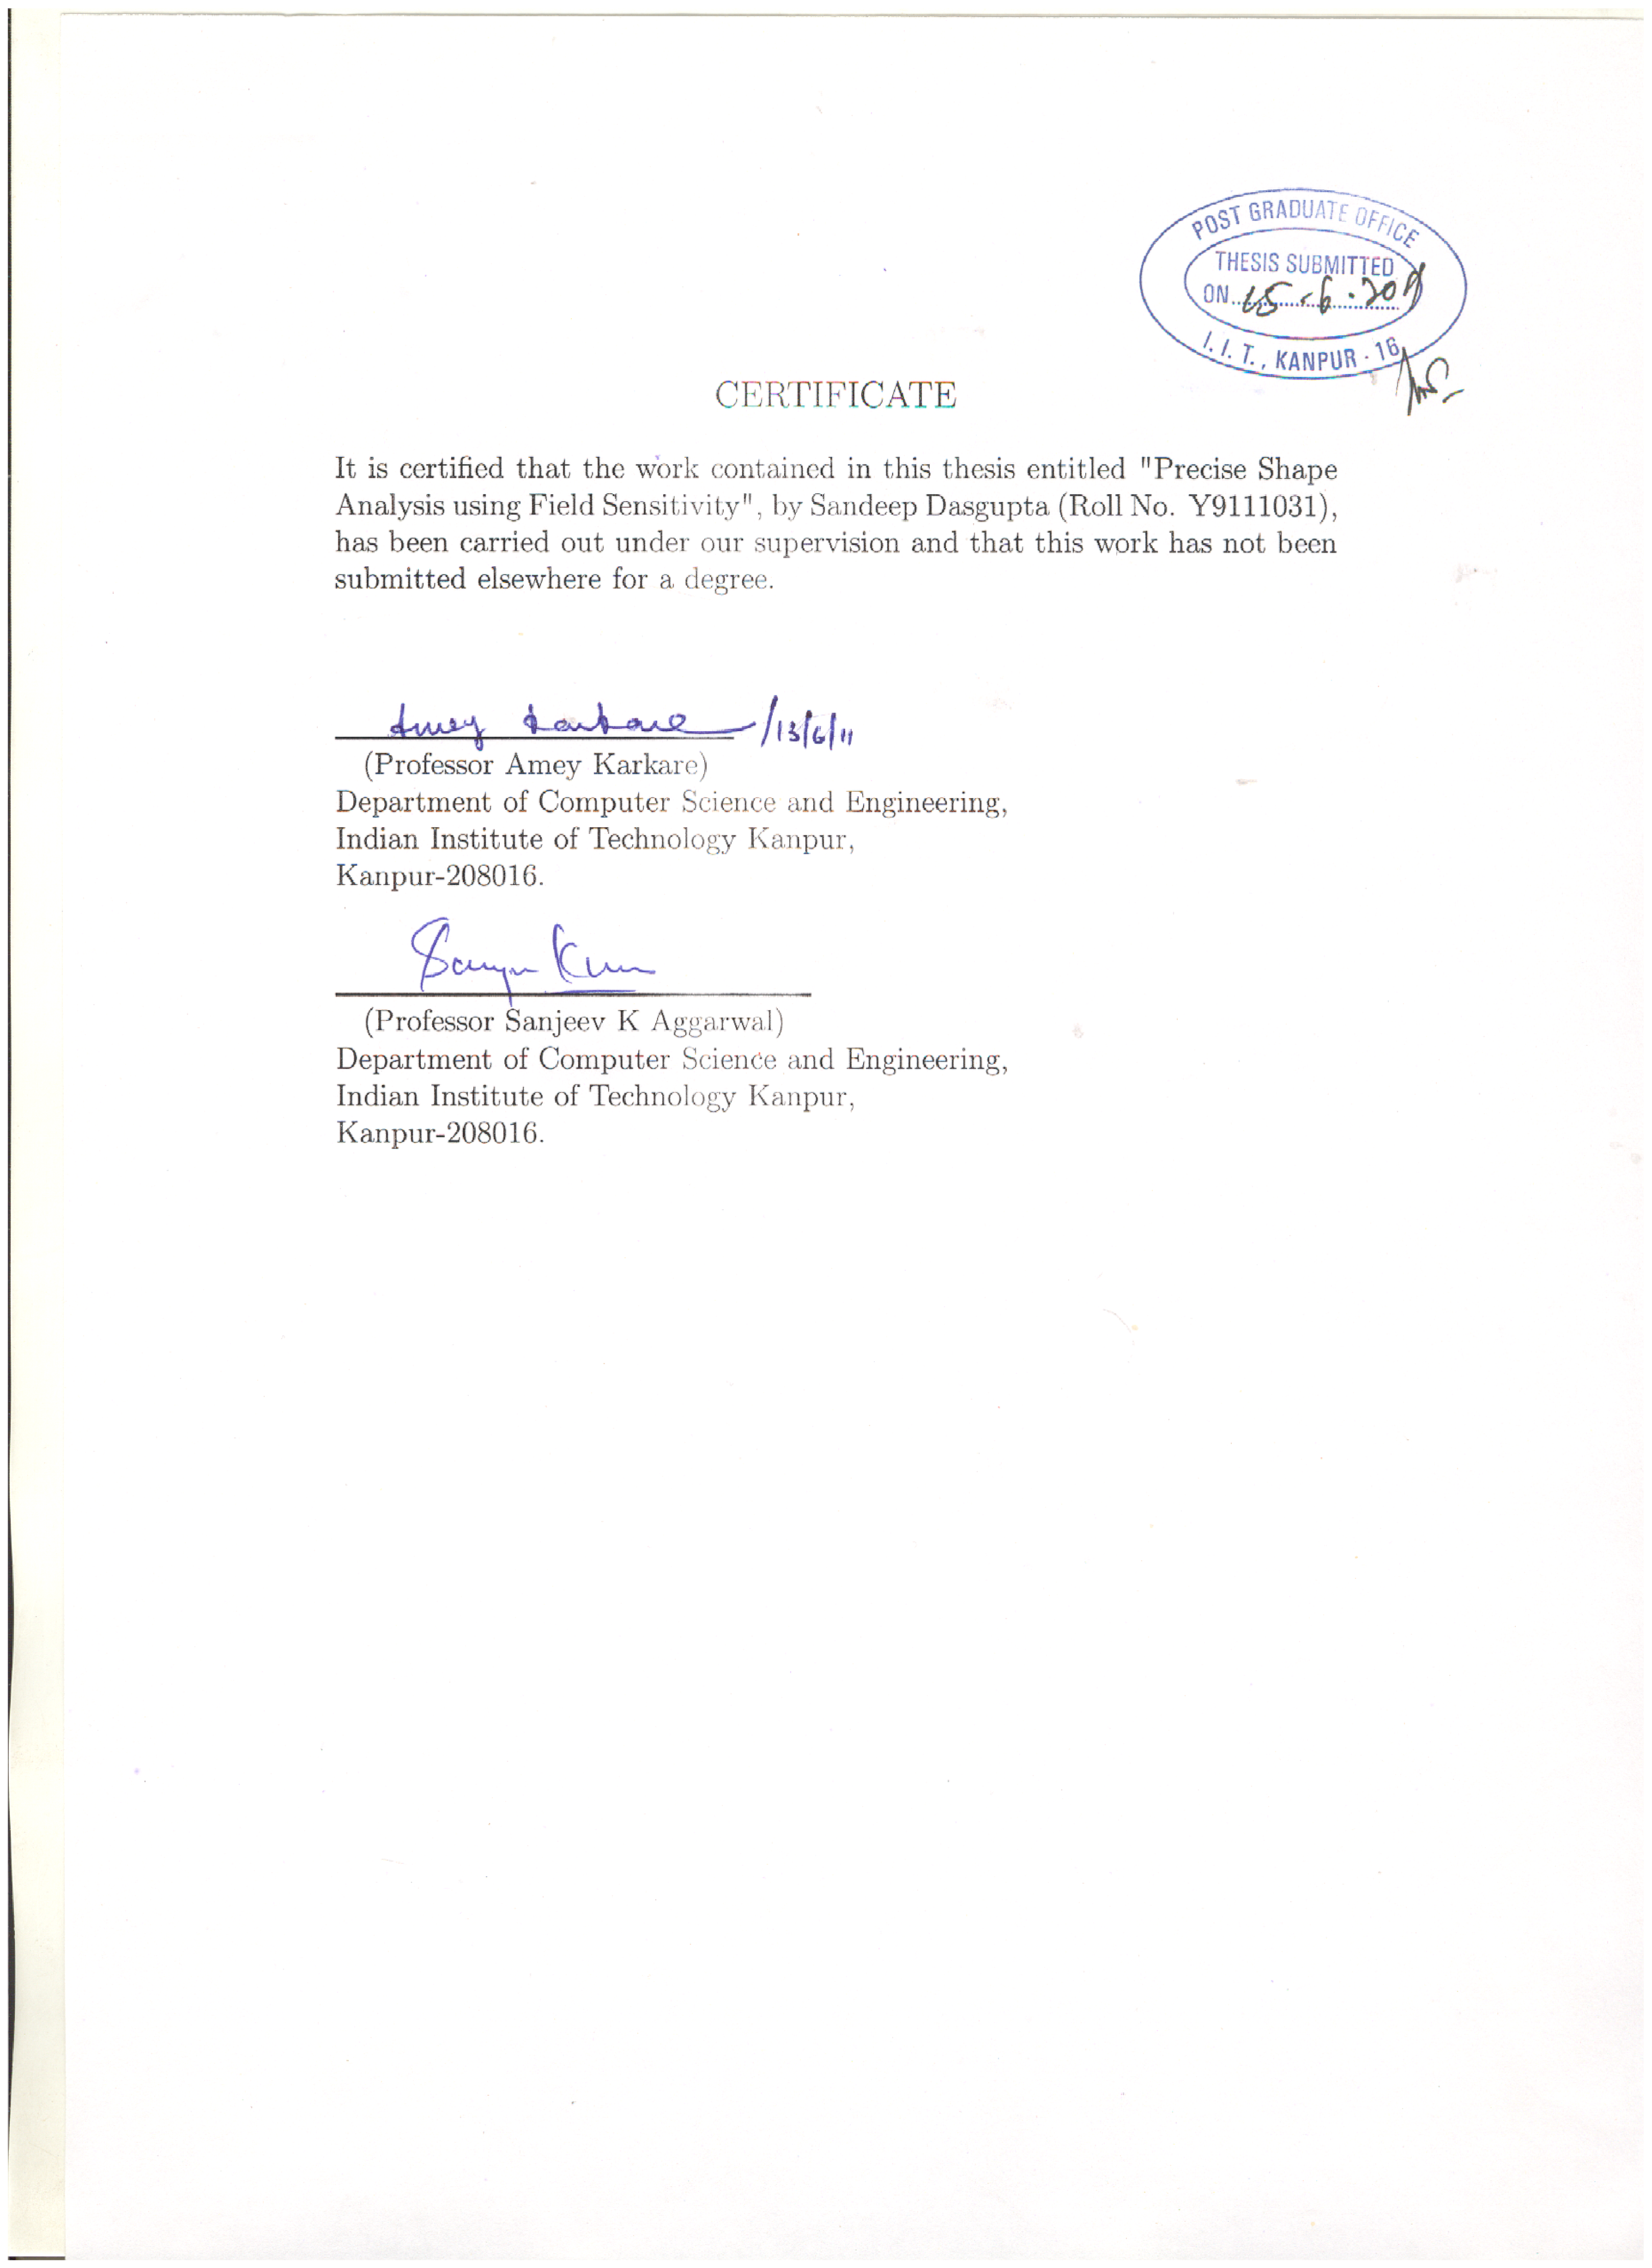
\includegraphics[width=\textwidth]{Figure/dsand.eps}
\vspace{2in}
\begin{abstract}
Programs in high level languages make intensive use of heap
to support dynamic data structures.  Analyzing these programs
requires precise reasoning about the heap structures. Shape
analysis refers to the class of techniques that statically
approximate the run-time structures created on the heap.  In
this work, we present a novel field sensitive shape analysis
technique to identify the shapes of the heap structures.  The
novelty of our approach lies in the way we use field
information to remember the paths that result in a particular
shape (Tree, DAG, Cycle).  We associate the field information
with a shape in two ways: (a) through boolean functions that
capture the shape transition due to change in a particular
field, and (b) through matrices that store the field
sensitive path information among two pointer variables.  This
allows us to easily identify transitions from Cycle to DAG,
from Cycle to Tree and from DAG to Tree, thus making the
shape more precise.
\end{abstract} 
 
\newpage
\begin{center}
\thispagestyle{empty}
\vspace*{2in}
{\it This thesis is dedicated\\
to my sister Mousumi Dasgupta.}
\end{center}
\chapter*{Acknowledgment}
\vspace{1.0in}
I would like to express my heartiest gratitude towards my thesis supervisor {\bf Professor Amey Karkare}
 for his invaluable support and encouragement. His guidance has helped
me from initial till the final level of this work on the way developing a sound
understanding of the topic. It would have been very difficult for me to complete
this work without his innumerable innovative suggestions, the freedom that he has
provided and his utmost patience in hearing my problems out. Apart from gaining a lot from 
his huge technical expertise, starting from gaining tips about how to write a good report to 
getting insights whenever I got struck, I got many learnings which I will explore throughout my life. \\
%%
I wish to thank {\bf Prof. Sanjeev K. Aggarwal}, for his 
immense support and invaluable suggestions 
that I have received from him. \\
I would also like to thank {\bf Prof. Subhajit Roy} for 
all the enriching discussions that I had with him.\\
%%
%In the preparation of this report, I had to consult constantly 
%various papers, articles and journals. I, hereby, acknowledge 
%my indebtedness to them all. \\
%%
Special thanks to my friend and fellow mate 
{\bf Ms. Barnali Basak} for her encouragement and enormous 
help and lots of thanks to my institution without which this 
thesis would have been a distant reality. \\
%%
Finally, I wish to extend my thanks to my parents, my sister and my beloved 
friends, who have always been a source of inspiration 
and encouragement. Their love and blessings have always 
been a driving force in my life to carry all my works 
with hope and optimism.\\
%%
Every effort has been made to give credit where it is due for
the material contained here in. If inadvertently I have
omitted giving credit to anyone, I apologize and express my
gratitude for their contribution to this work. 
\begin{flushright} \large
\textit{Sandeep Dasgupta}\\
\textit{June 2011}\\
\textit{Indian Institute of Technology, Kanpur}\\
\end{flushright}
\newpage

%
\thispagestyle{empty}
%\chapter*{Declaration}
\vspace*{5cm}
\begin{center}
\underline{\textbf{Declaration}}
\end{center}

I declare that this written submission represents my ideas in my own 
words except Appendix A and B whose contents are borrowed from Ghiya et. al.~\cite{Ghiya96} and Marron et. al.~\cite{marron06static} respectively for the 
ease of reference. The places where others' ideas or words have been included, I have adequately cited and 
referenced the original sources.
\newpage

%
\pagenumbering{roman}
\tableofcontents
\listoffigures
\listoftables
\newpage

\pagenumbering{arabic}
\chapter{Introduction}
\label{ch:Intro}
In the recent arena of parallel architectures (multi-cores,
GPUs, etc.), software side lags behind hardware. This is due to the reason that dealing with 
parallelism adds a new dimension to the design of programs, therefore 
makes it complex. One approach for efficient parallelization of programs is to explicitly 
induce parallelism. It includes designing of concurrent programming languages like Go, X10 etc., 
libraries, APIs like POSIX, OpenMP, Message 
Passing Interface(MPI) etc. The main advantage of such approach is that it gives simple and clear directions to the 
compiler to parallelize the code. But the main drawbacks of such approach is that the degree of parallelism totally depends upon 
the efficiency of programmer and imposing external parallelism turns the code into legacy one. 
The other approach is to automatically 
parallelizing sequential programs by compiler which extract parallelism 
without violating correctness. This is a key step in increasing
the performance and efficiency. 
%
\section{Motivation}
Over the past years, lot of work has been done on automatically 
parallelizing sequential programs. These approaches have mainly 
been developed for programs having only static data structures 
(fixed sized arrays) and written in languages such as FORTRAN
~\cite{Allen87automatic,Banerjee93automatic,Wolf91loop,
  Kennedy01Optimizing}. Almost all programming languages
today use the heap for dynamic recursive data structures. 
\begin{comment}
The basic building block of such structure is node which consists 
of one or more fields. Each field is designated as a scalar field or 
pointer field. A pointer field contains either \emph{null} value or pointer to 
a node of the same type. 
\end{comment}

Therefore, any parallelization must also take into account the data
dependency due to the access of common heap nodes of such 
structures. Finding parallelism in sequential programs written
in languages, with dynamically allocated data structures, such
as C, C++, JAVA, LISP etc., has been less successful. One of
the reason being the presence of pointer-induced aliasing,
which occurs when multiple pointer expressions refer to same
storage location. Compared to the analysis of static and
stack data, analyzing properties of heap data is challenging
because the structure of heap is unknown at compile time. It
is also potentially unbounded and the lifetime of a heap
object is not limited by the scope that creates it. As a
consequence, properties of heap (including dependence) are
approximated very conservatively. The approximation of the
heap data dependence information inhibits the parallelization. 

The objective of our analysis is to detect both coarse-grained parallelism 
in the context of function calls, loops and fine-grained parallelism in the 
context of statements. We show the following two examples as motivating 
examples of our work.
\begin{figure}[t]
  \begin{center}
  
    \scalebox{.85}{\begin{tabular}{ c | c }
%    \hline
 	& \multirow{3}{*}{ {\tt
\begin{program}{0}
%  \FL\ \ldots
  \UNL{0} void treeAdd(tree t) \{
  \UNL{1}  if(t == NULL)
  \UNL{2} return;
  \NL{1}     tl = t$\rightarrow$left;
  \NL{1}     treeAdd(tl);
  \NL{1}     tr = t$\rightarrow$right;
  \NL{1}     treeAddd(tr);
  \UNL{1}	t\rtarrow{num} = tl\rtarrow{num} + tr\rtarrow{num};
  \UNL{0} \}
\end{program}
}} \\
%    & \\
      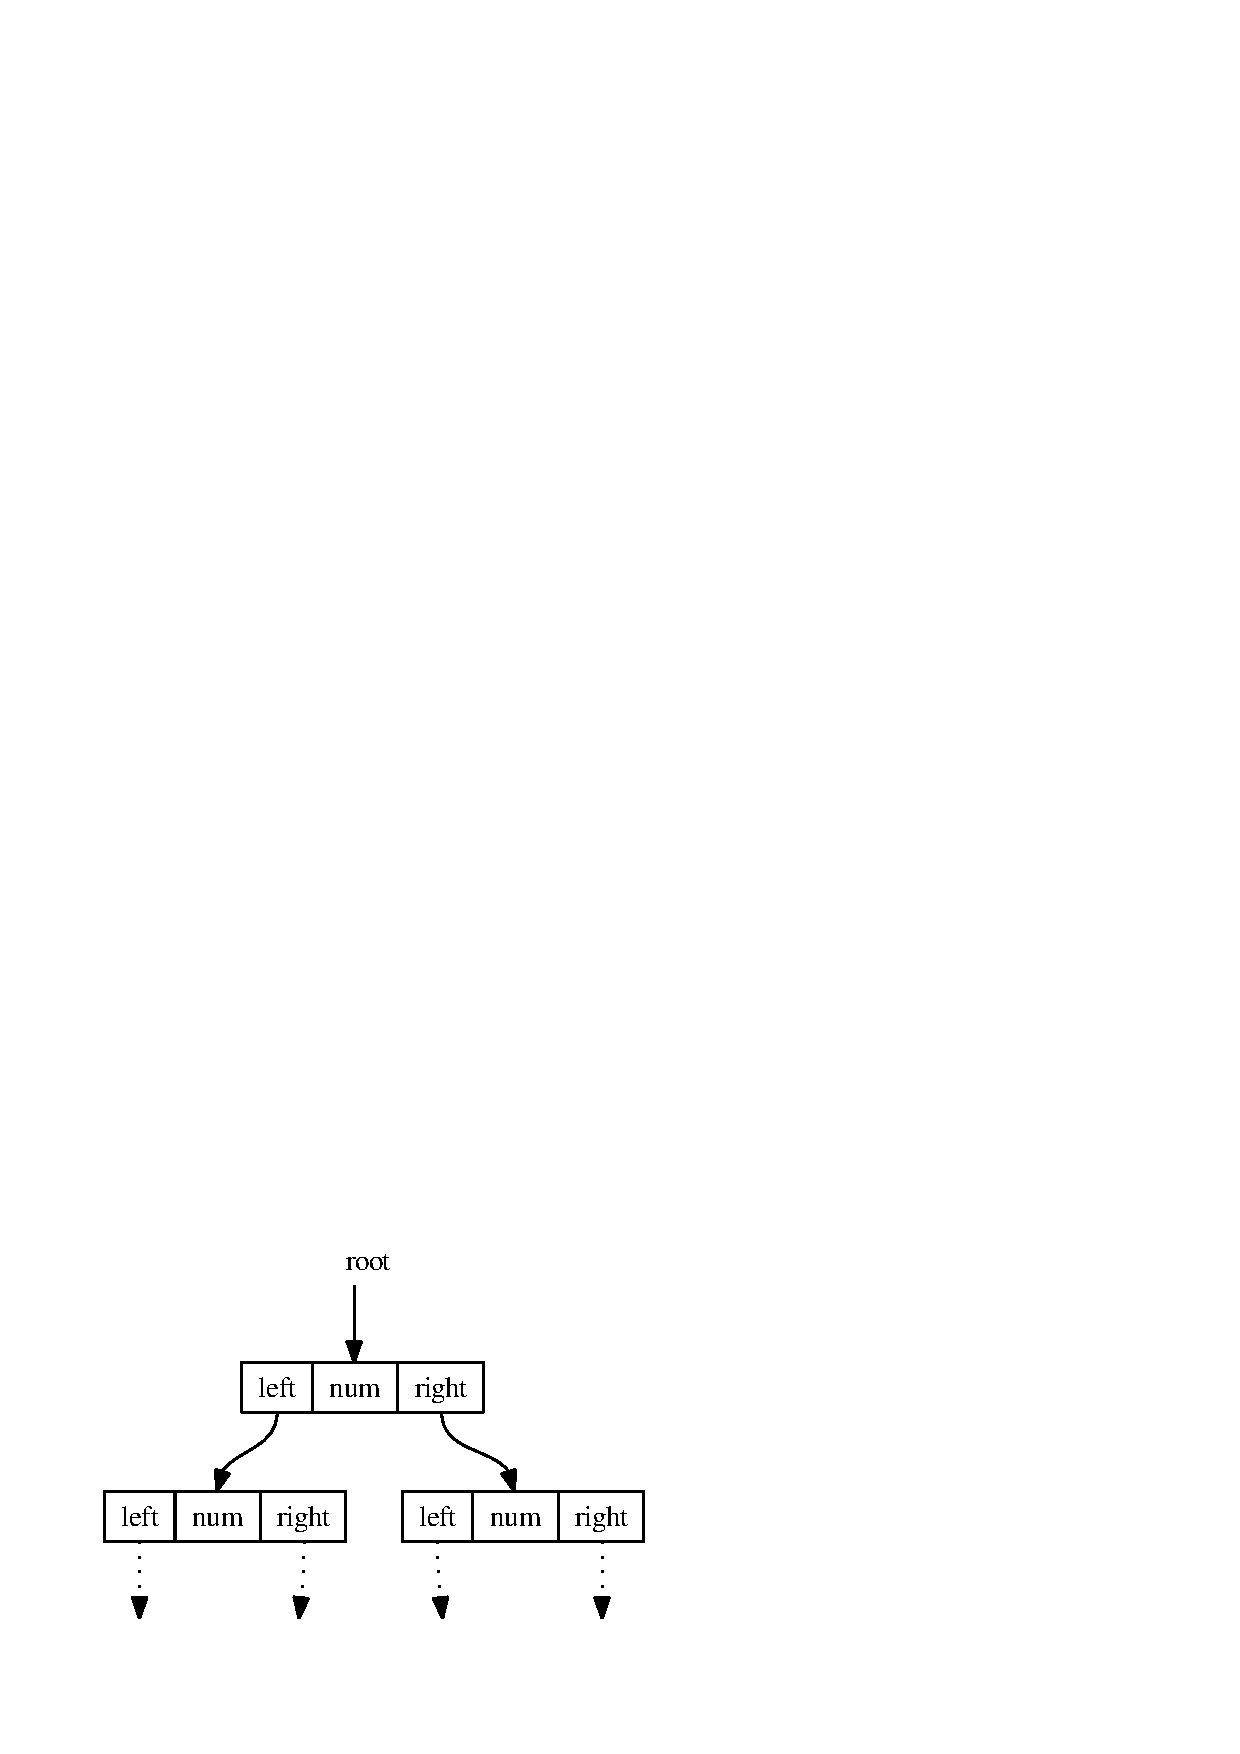
\includegraphics[scale=0.6]{tree_grph}
      & \\
%      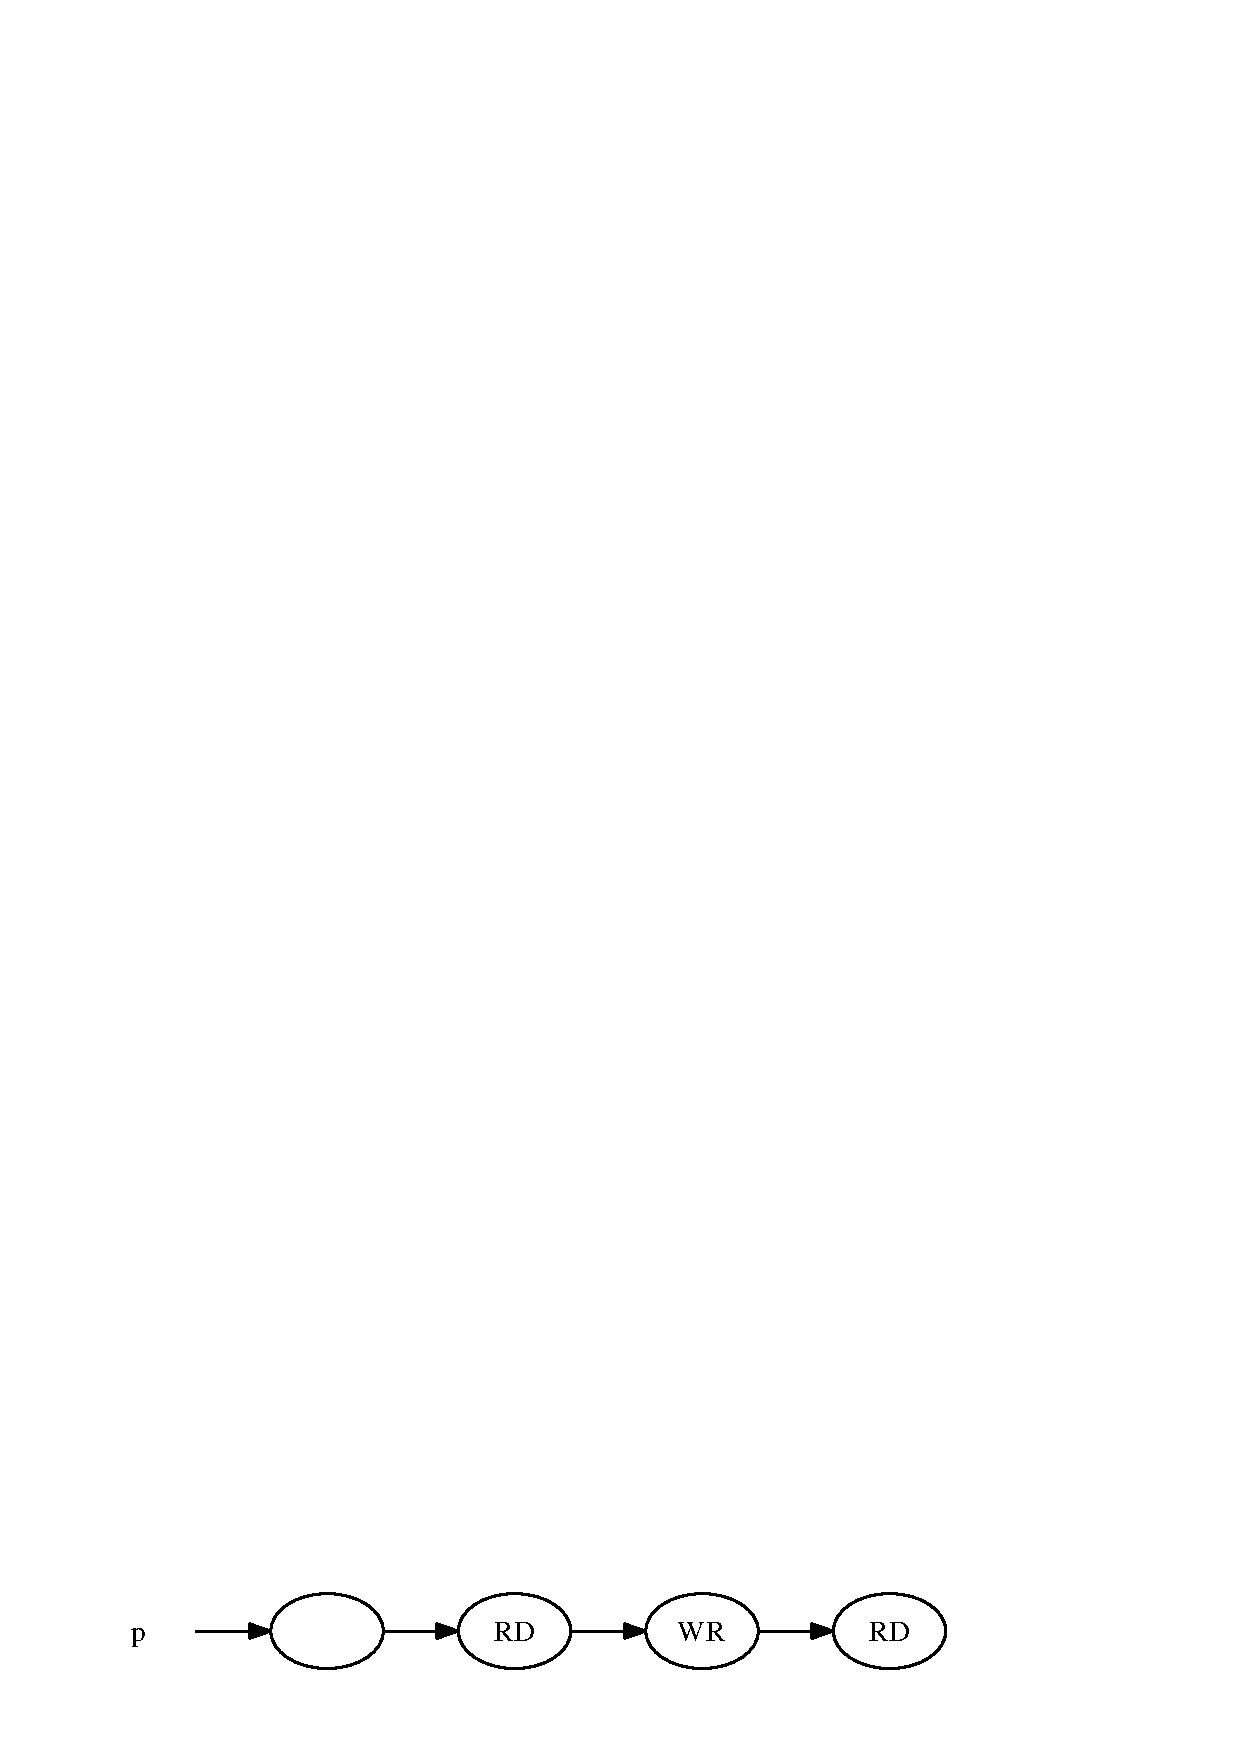
\includegraphics[scale=0.6]{grph_motiv} & \\
%      (a) & (b) \\
     (a) Data structure & 
     (b) Function traversing the data structure. \\
%    \hline 
    \end{tabular}}
  \end{center}
  \hrule
  \caption{\label{fig:motiv1} Motivating example: function-call parallelization}
%\hrule
\end{figure}
\begin{example}{\rm 
Consider Figure~\ref{fig:motiv1} which gives a motivational 
example for parallelism in the context of function calls. It shows 
the tree data 
structure and the function \emph{treeAdd} traversing on the 
data structure. In the code fragment the two calls to the function 
\emph{treeAdd} respectively perform the additions of left and right 
subtrees recursively. If the analysis can ensure that the two function calls 
do not access any common region of heap, they can be executed in parallel.
} 
\hfill\psframebox{}  
\end{example}
%%%%%%%%%%%%%%%%%
\begin{figure}[t]
  \begin{center}
  
    \scalebox{.85}{\begin{tabular}{ c | c }
 %   \hline
      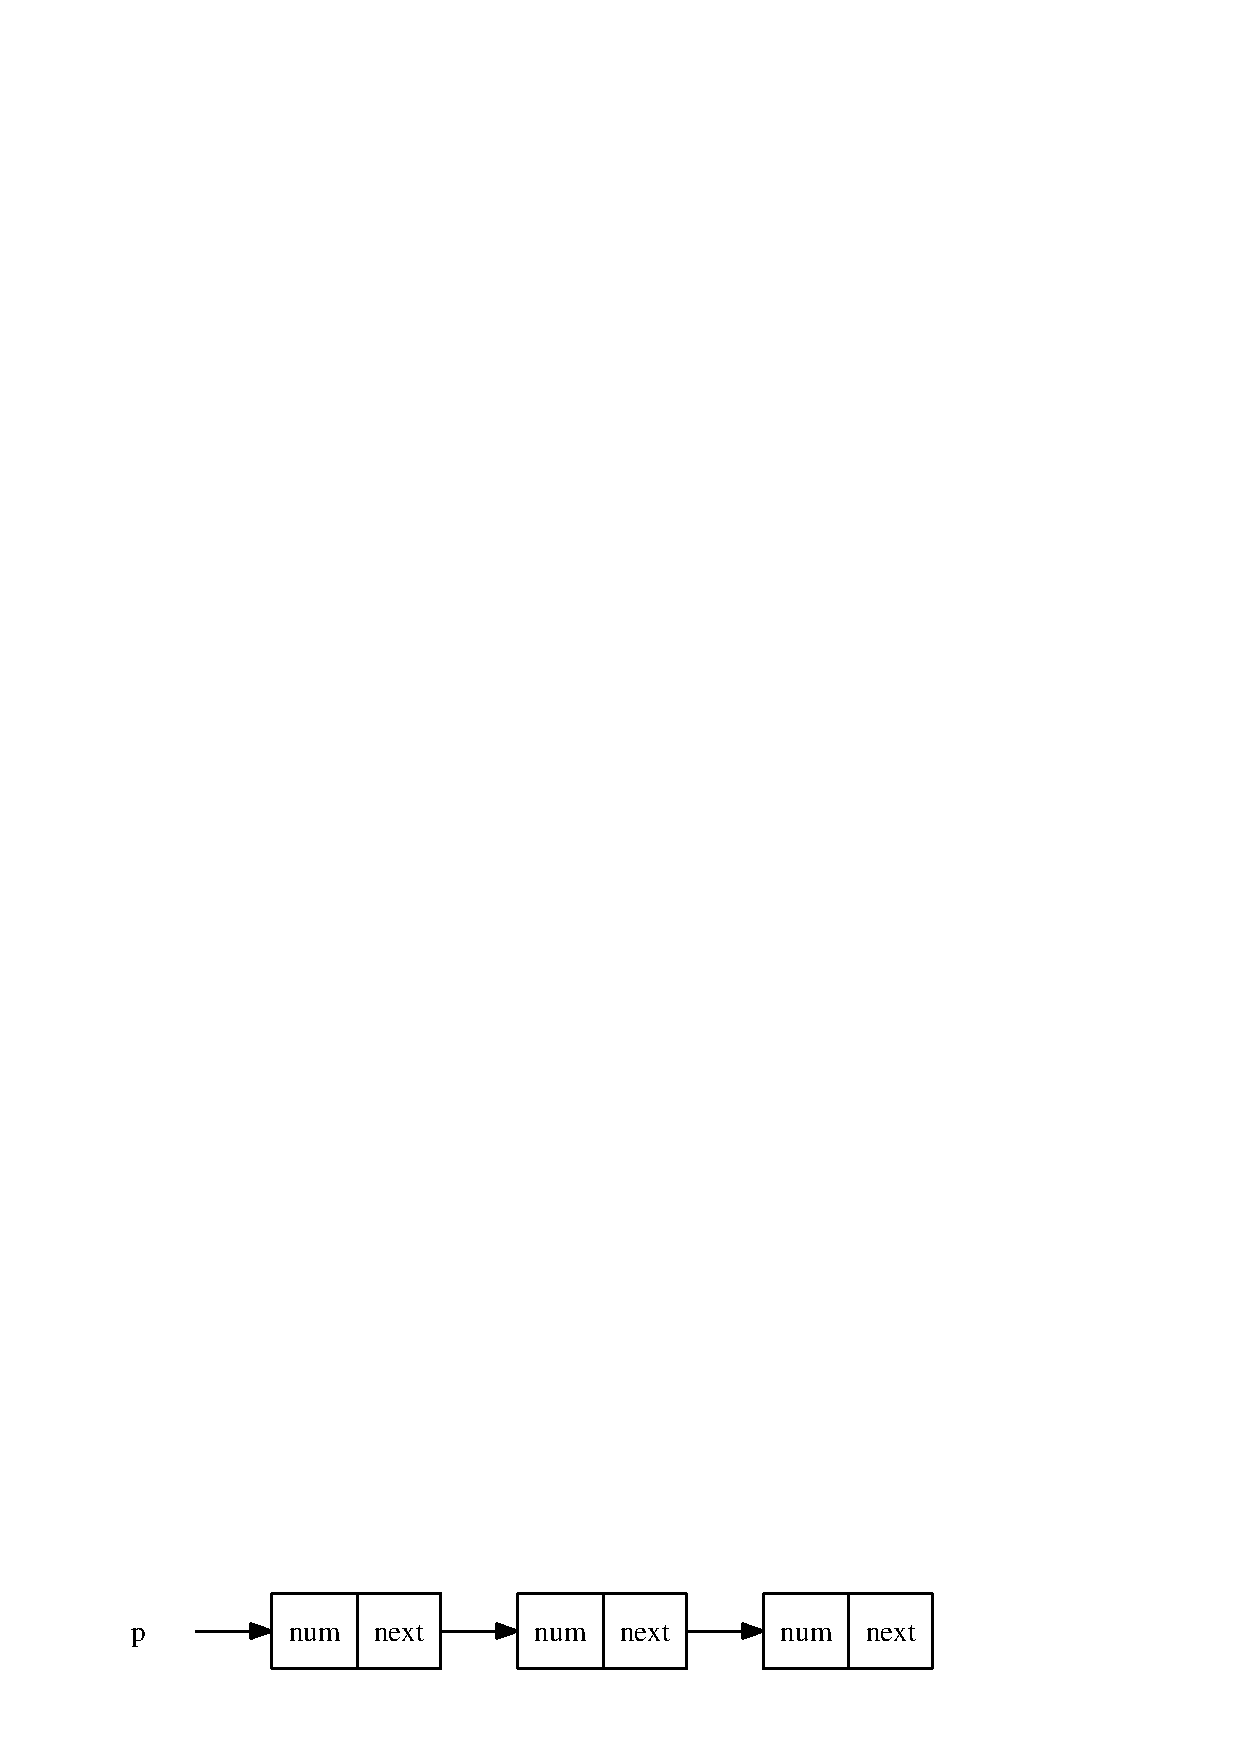
\includegraphics[scale=0.6]{grph4} %\cline{1-1}
      &
      {\tt
\begin{program}{0}
  \FL\ \ldots
  \NL{0} p = list;
  \UNL{0} \WHILE (p$\rightarrow$next != NULL) \{
  \NL{1}     q = p$\rightarrow$next;
  \NL{1}     temp = q$\rightarrow$num;
  \NL{1}     r = q$\rightarrow$next;
  \NL{1}     r$\rightarrow$num = temp;
  \NL{1}     p = r;
  \UNL{0} \}
  \UNL{0} \ldots
\end{program}
} \\
      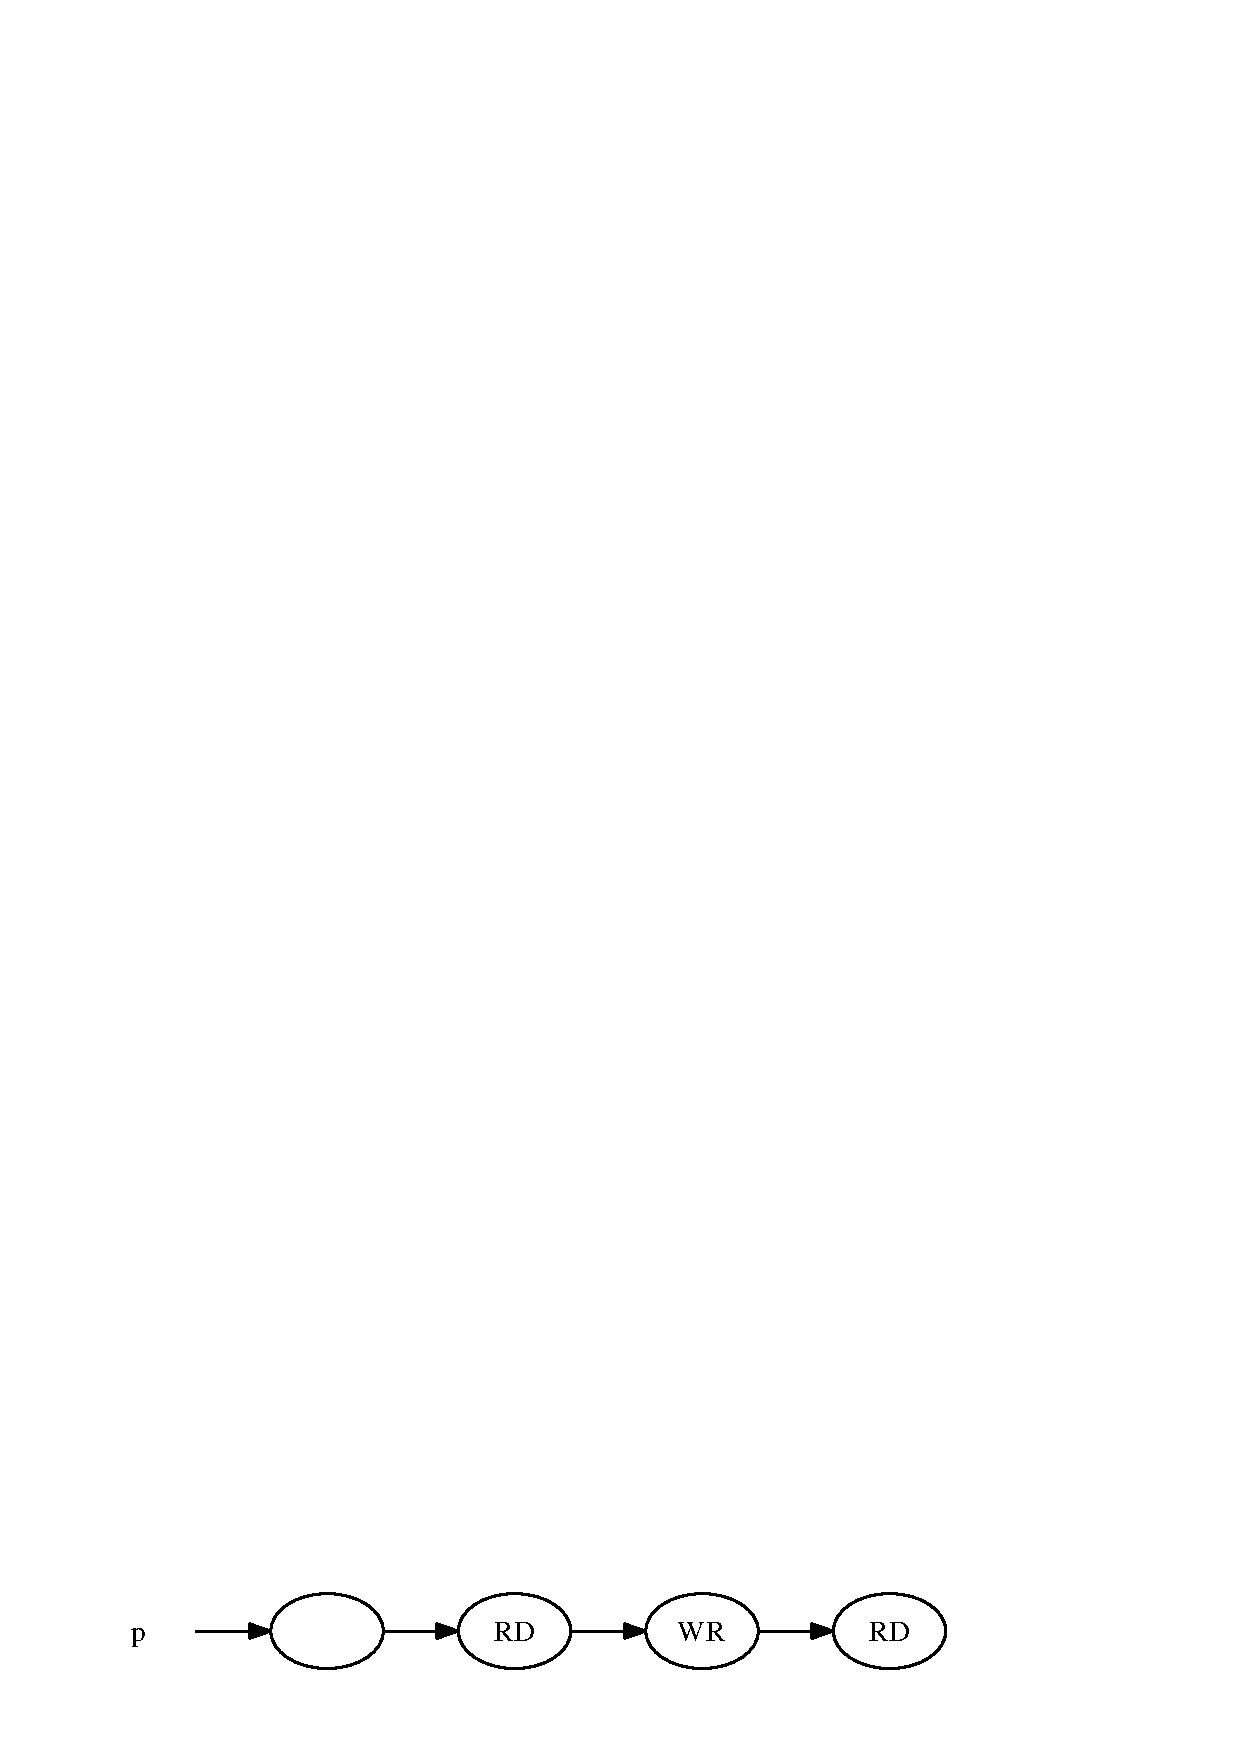
\includegraphics[scale=0.6]{grph_motiv} & \\
%      (a) & (b) \\
     (a) Nodes read and written by code & 
     (b) Loop traversing the data structure. \\
    \end{tabular}}
  \end{center}
  \hrule
  \caption{\label{fig:motiv} Motivating example: loop parallelization}
%\hrule
\end{figure}
\begin{example}{\rm
  Figure~\ref{fig:motiv}
  shows an example of loop level parallelism. It shows list data structure and the nodes of the structure being read and written, tagged by \emph{Read} (\ttf{RD}) 
  and \emph{Write} (\ttf{WR}) access by the code fragment traversing the
  data structure. Note that, the first node of the structure is a special node which is neither 
  read nor written by the code fragment. The performance of the code can be improved if the loop can
  be executed in parallel. However, without the knowledge of
  precise heap dependences, we have to assume worst case
  scenario, i.e.,  the  location read by the statement {\tt
    S3} in some iteration could be the same as the location
  written by the statement {\tt S5} in some other iteration.
  In that case,  it is not possible to parallelize the loop.
 
  Our dependence analysis can show that the locations read by
  {\tt S3} and those written by {\tt S5} are mutually
  exclusive. Further, it also shows the absence of any other
  dependences.  This information, along with the information
  from classical control and data dependence analysis, can be
  used by a parallelizing compiler to parallelize the loop.
}
\hfill\psframebox{}  
\end{example}

This report explains our approach for a practical heap data dependence analysis. 
As it is understood that we are only talking about data dependences, we drop the term 
data in the rest of the report. 
%
\section{Contributions of our Work}
Our work contributes in the area of heap based 
dependence analysis. We present a novel approach 
which identifies dependences and extracts parallelism for a sequential program. 
In particular, our approach finds out dependences between two statements. 
This enables us to find out whether two procedure calls 
access disjoint structures, hence can be executed in parallel. 
Then we refine this technique to work better 
in presence of loops. We also extend the work of loop analysis 
for static and scalar data to support heap intensive loops.

\section{Organization of the Thesis}
The rest of the thesis is organised as follows. We discuss about related 
work done in the field of heap intensive dependence analysis in Chapter~\ref{ch:RelatedWork}.
Chapter~\ref{ch:back} specifies the imperative programming model 
for which our analysis is defined and gives the other background 
details. Chapter~\ref{ch:dep} through~\ref{ch:interdep} provide a complete 
description of our practical dependence analysis applied to 
dynamically allocated structure. Chapter~\ref{ch:dep} gives the detailed 
explanation of the intra-procedural dependence detection technique 
which separately works on each procedure of a program. Chapter~\ref{ch:loopdep} 
presents our method to handle loops in a more specific way. We also 
give the inter-procedural framework for our analysis in Chapter~\ref{ch:interdep}. 
Chapter~\ref{ch:result} demonstrates our whole method by extensively 
analysing few benchmark codes. We conclude the report in Chapter~\ref{ch:conclusion} 
by giving the direction for future research.
\chapter{Related Work} \label{ch:RelatedWork}
The shape-analysis problem was initially studied in the
context of functional languages. Jones and
Muchnick~\cite{Jones79} proposed one of the earliest shape
analysis technique for Lisp-like languages with destructive
updates of structure. They used sets of finite shape graphs
at each program point to describe the heap structure.  To
keep the shape graphs finite, they introduced the concept of
$k$-limited graphs where all nodes beyond $k$ distance from
root of the graph are summarized into a single node. Hence
the analysis resulted in conservative approximations. The
analysis is not practical as it is extremely costly both in
time and space .

Chase et al.~\cite{Chase90} introduced the concept of limited
reference count to classify heap objects into different
shapes. They also classified the nodes in concrete and
summary nodes, where summary nodes were used to guarantee
termination. Using the reference count and concreteness
information of the node, they were able to kill relations
({\em strong updates}) for assignments of the form $\p\rightarrow f = \q$
in some cases. However, this information is not
insufficient to compute precise shape, and detects false
cycle even in case of simple algorithms like destructive list
reversal.

Sagiv et. al.~\cite{Sagiv96,Sagiv99,Sagiv02toplas} proposed
generic, unbiased shape analysis algorithms based on {\em
  Three-Valued} logic. They introduce the concepts of {\em
  abstraction} and {\em re-materialization}. Abstraction is
the process of summarizing multiple nodes into one and is
used to keep the information bounded.  Re-materialization is
the process of obtaining concrete nodes from summary node and
is required to handle destructive updates. By identifying
suitable predicates to track, the analysis can be made very
precise.  However, the technique has potentially exponential
runtime in the number of predicates, and therefore not
suitable for large programs.


Distefano et al.~\cite{distefano06local} presented a shape
analysis technique for linear data structures (linked-list
etc.), which works on symbolic execution of the whole program
using separation logic. Their technique works on suitable
abstract domain, and guarantees termination by converting
symbolic heaps to finite canonical forms, resulting in a
fixed-point. By using enhanced abstraction scheme and
predicate logic, Cherini et al.~\cite{cherini10shape}
extended this analysis to support nonlinear data structure
(tree, graph etc.).

Berdine et al.~\cite{berdine07shape} proposed a method for
identifying composite data structures using generic
higher-order inductive predicates and parameterized spatial
predicates.  However, using of separation logic does not
perform well in inference of heap properties.  Hackett and
Rugina in~\cite{hackett05region} presented a new approach for
shape analysis which reasons about the state of a single heap
location independently. This results in precise abstractions
of localized portions of heap. This local reasoning is then
used to reason about global heap using context-sensitive
inter-procedural analysis.  Cherem
et. al.~\cite{cherem07doubly} use the local abstraction
scheme of~\cite{hackett05region} to generate local invariants
to accurately compute shape information for complex data
structures.  

Jump and McKinley~\cite{maria09dynamic} give a technique for
dynamic shape analysis that characterizes the shape of
recursive data structure in terms of dynamic degree metrics
which uses in-degrees and out-degrees of heap nodes to
categorize them into classes. Each class of heap structure is
then summarized. While this technique is useful for detecting
certain types of errors; it fails to visualize and understand
the shape of heap structure and cannot express the sharing
information in general.

Our work is closest to the work proposed by Ghiya
et. al.~\cite{Ghiya96} and by Marron
et. al.~\cite{marron06static}.  Ghiya et al.~\cite{Ghiya96}
keeps interference and direction matrices between any two
pointer variables pointing to heap object and infer the shape
of the structure as Tree, DAG or Cycle. They have also
demonstrated the practical applications of their
analysis~\cite{Ghiya96practicaltechniques,Ghiya98a,Ghiya98b} and shown that it works well on practical
programs. However, the main shortcoming of this approach is
it cannot handle kill information. In particular, the
approach is unable to identify transitions from Cycle to DAG,
from Cycle to Tree and from DAG to Tree. So it has to to
conservatively identify the shapes.

Marron et. al.~\cite{marron06static} presents a data flow
framework that uses heap graphs to model data flow
values. They presented an abstract heap model that can represent 
information on aliasing, shape, logical data structures, sharing between variables, 
and sharing between data elements in collections.
They introduce a restricted version of refinement, based on the ideas presented by Sagiv,
Reps and Wilhelm. Using this restricted notion of refinement, they demonstrate how this 
model can be used to accurately simulate important program events such as list copying, sorting, reversal,
and various other destructive operations. 
The analysis uses technique similar to
re-materialization, but unlike parametric shape analysis
techniques~\cite{Sagiv99,Sagiv02toplas}, the
re-materialization is approximate and may result in loss of
precision. 

Our method is also data flow analysis framework, that uses
matrices and boolean functions as data flow values. We use
field sensitive connectivity matrices to store path
information, and boolean variables to record field
updates. By incorporating field sensitivity information, we
are able to improve the precision without much impact on
efficiency. The next chapter presents a simplified view of
our approach before we explain it in full details.

As our work is closest to the work of Ghiya
et. al.~\cite{Ghiya96} we present a brief summary of their
analysis in Appendix A.

\cmt{
%%%%%%%%%%%%%%%%%%%%%%%%%%%%%%%%%%%%%%%%%%%%%%%%%%%%%%%%%%%%%%%%%%%%%%
\section[Analysis of Ghiya et. al.~\cite{Ghiya96}]{Analysis of Ghiya et. al.~\cite{Ghiya96}\footnote{The contents of this section are borrowed from ~\cite{Ghiya96}}}
%%%%%%%%%%%%%%%%%%%%%%%%%%%%%%%%%%%%%%%%%%%%%%%%%%%%%%%%%%%%%%%%%%%%%%
Their shape analysis composed of three store-less
abstractions that are computed together at each program point.
For each heap directed pointer they approximated the attribute
shape and for each pair of heap directed pointers they approximated the 
direction and interference relationships between them. These three abstractions 
are defined formally as follows:

\begin{definition}
Given any heap-directed pointer $p$, the shape attribute p.shape is Tree, 
if in the data structure accessible from p there is a unique (possibly empty) access path 
between any two nodes (heap objects) belonging to it. It is considered to be DAG (directed acyclic graph), 
if there can be more than one path between any two nodes in this data structure, 
but there is no path from a node to itself (i. e, it is acyclic). 
If the data structure contains a node having a path to itself, p.shape is considered to be Cycle.
Note that as lists are special case of tree data structures, their shape is also considered as Tree.
\end{definition}

\begin{definition}
Given two heap directed pointers $p$ and $q$, the direction matrix $D$ captures the following 
relationships between them:
\begin{itemize}
\item $D[p,q] = 1 : $ An access path possibly exists in the heap, from the heap object pointed to by $p$,
to the heap object pointed to by $q$. In this case we simply say that the pointer $p$ has a path to 
pointer $q$.
\item $D[p,q] = 0 : $ No access path exists from the heap object pointed to by $p$ to the heap object pointed to by $q$. 
\end{itemize}
\end{definition}

\begin{definition}
Given two heap directed pointers $p$ and $q$, the direction matrix $I$ captures the following 
relationships between them:
\begin{itemize}
\item $I[p,q] = 1 : $ A common heap object can be possibly accessed starting from pointers $p$ and $q$.
In this case we state that pointers $p$ and $q$ can interfere.
\item $I[p,q] = 0 : $ No common heap object can be accessed starting from pointers $p$ and $q$.
In this case we state that pointers $p$ and $q$ do not interfere.
\end{itemize}
\end{definition}

Direction relationships are used to actually estimate the shape attributes, where the interference 
relationships are used for safely calculating direction relationships. 

\subsection{Illustrative Example}

The direction and interference matrices are illustrated in Fig.~\ref{fig:relwork_1}.
Part (a) represents a heap structures at a program point, while parts (b) and (c) show the direction 
and interference matrices for it.  
\begin{figure}
\centering
\begin{tabular}{c@{$\qquad\qquad$}c}
\multicolumn{2}{c}{
\scalebox{0.80} { 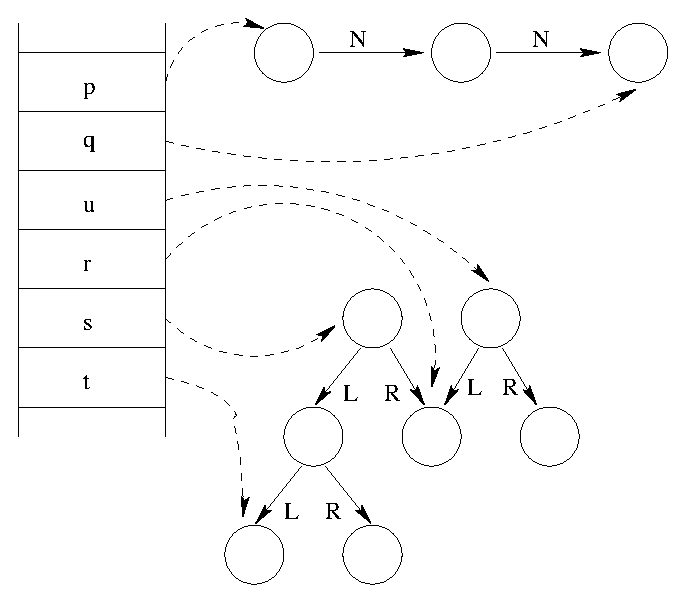
\includegraphics[scale=1]{diagrams/Appendix_2.eps}}
} \\
\multicolumn{2}{c}{
\scalebox{0.80}{ (a) Heap Structure }
} \\ \\
\scalebox{0.80} { \begin{tabular}{|c||c|c|c|c|c|c|}
\hline
$D$ & $p$ & $q$ & $r$ & $s$ & $t$ & $u$ \\ \hline \hline
$p$ & $1$ & $1$ & $0$ & $0$ & $0$ & $0$ \\ \hline 
$q$ & $0$ & $1$ & $0$ & $0$ & $0$ & $0$ \\ \hline 
$r$ & $0$ & $0$ & $1$ & $0$ & $0$ & $0$ \\ \hline 
$s$ & $0$ & $0$ & $1$ & $1$ & $1$ & $0$ \\ \hline 
$t$ & $0$ & $0$ & $0$ & $0$ & $1$ & $0$ \\ \hline 
$u$ & $0$ & $0$ & $1$ & $0$ & $0$ & $1$ \\ \hline 
\end{tabular}} 
& 
\scalebox{0.80} {\begin{tabular}{|c||c|c|c|c|c|c|}
\hline
$I$ & $p$ & $q$ & $r$ & $s$ & $t$ & $u$ \\ \hline \hline
$p$ & $1$ & $1$ & $0$ & $0$ & $0$ & $0$ \\ \hline 
$q$ & $1$ & $1$ & $0$ & $0$ & $0$ & $0$ \\ \hline 
$r$ & $0$ & $0$ & $1$ & $1$ & $0$ & $1$ \\ \hline 
$s$ & $0$ & $0$ & $1$ & $1$ & $1$ & $1$ \\ \hline 
$t$ & $0$ & $0$ & $0$ & $1$ & $1$ & $0$ \\ \hline 
$u$ & $0$ & $0$ & $1$ & $1$ & $0$ & $1$ \\ \hline 
\end{tabular}}  \\
\scalebox{0.80}{ (b) Direction Matrix}  & \scalebox{0.80} {(c) Interference Matrix}
\end{tabular}
\caption{Example Direction and Interference Matrices}
\label{fig:relwork_1}
\end{figure}


We now demonstrate how direction relationships help estimate the shape of the data structures.
In Fig.~\ref{fig:relwork_2}, initially we have both \p.\shape\ and \q.\shape\ as Tree. Further $D[q,p] == 1$, as there 
exists a path from \q\ to \p\ through {\tt next} link. The statement {\tt p$\rightarrow$prev = q}, sets up a path from
\p\ to \q\  through the {\tt prev} link. From direction matrix information we already know that a path exists
from \q\ to \p, and now a path is being set from \p\ to \q. Thus after the statement, $D[p,q] = 1$, $D[q,p] = 1$, \p.\shape\ = Cycle
and \q.\shape\ = Cycle.  

\begin{figure}
\centering
\scalebox{.80} {
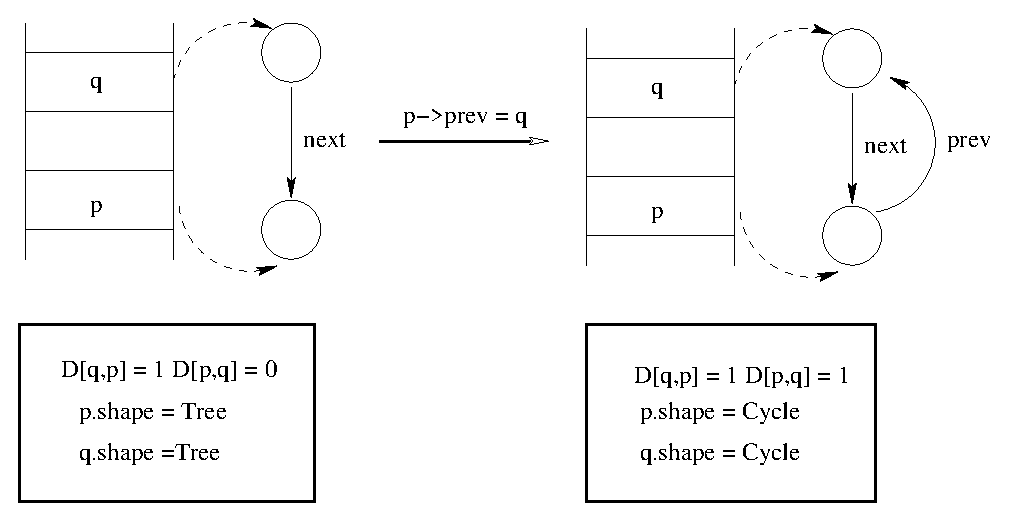
\includegraphics[scale=1]{Figure/figure_3}
}
\caption{Example Demonstrating Shape Estimation}
\label{fig:relwork_2}
\end{figure}

\subsection{Analysis of Basic Statements}
They have considered eight basic statements that can access or
modify heap data structures as listed in Fig.~\ref{fig:relwork_3}(a). Variables \p\ and \q and the field $f$ are
of pointer type, variable $k$ is of integer type, and $op$ denotes the $+$ and $-$ operations. The 
overall structure of the analysis is shown in Fig.~\ref{fig:relwork_3}(b). Given the direction and the interference 
matrices $D$ and $I$ at a program point x, before the given statement, they compute the matrices $D_n$ and $I_n$
at a program point y. Additionally, we have the attribute matrix A, where for a pointer $p$, $A[p]$ gives its shape attribute.
The attribute matrix after the statement is presented as $A_n$.

For each statement they compute the set of direction and interference relationships it kills and generates. Using these sets, the
new matrices $D_n$ and $I_n$ are computed as shown in Fig.~\ref{fig:relwork_3}(c). Note that the elements in the gen and kill sets are denoted as $D[p,q]$
for direction relationships, and $I[p,q]$ for interference relationships. Thus a gen set of the form $\{D[x,y], D[y,z]\}$, indicates that
the corresponding entries in the output direction matrix $D_n[x,y]$ and $D_n[y,z]$ should be set to one. We also compute the set of 
pointers $H_s$, whose shape  attribute can be modified by the given statement. Another attribute matrix $A_c$ is used to store the 
changed attribute of pointers belonging to the set $H_s$. The attribute matrix $A_n$ is then computed using the 
matrices $A$ and $A_c$ as shown in Fig.~\ref{fig:relwork_3}(c).  

Let $H$ be the set of pointers whose relationships/attributes are abstracted by the matrices $D$. $I$ and $A$. Further
assume that updating an interference matrix entry $I[\q,\p]$, implies identically updating the entry $I[\p,\q]$.   
\begin{figure}
\centering
\scalebox{0.90}{
\begin{tabular}{|c|c|c|}
\hline
\begin{tabular}{l}
Allocation \\
1. {\tt p = malloc();} \\
\\
Pointer Assignments \\
2. {\tt p = q;} \\
3. {\tt p = \&(q$\rightarrow$f);} \\
4. {\tt p = q op k;} \\
5. {\tt p = NULL;} \\
6. {\tt p = q$\rightarrow$f;} \\
\\
Structure Updates \\
7. {\tt p$\rightarrow$f = q;} \\
8. {\tt p$\rightarrow$f = NULL;}
\end{tabular}  &
\begin{tabular}{c}
\scalebox{0.80}{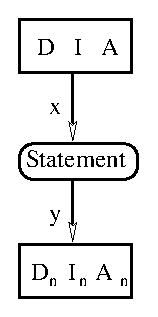
\includegraphics[scale=1]{diagrams/Appendix_4.eps}}
\end{tabular}
&
\begin{tabular}{l}
Build the new matrices\\
$\begin{array}{lll} 
\forall r,s \in H, & D_n[r,s] = D[r,s], & I_n[r,s] = I[r,s] \\
\forall s \in H, & A_n[s] = A[s]
\end{array}$ \\
\\
Delete Killed relationships \\
$\begin{array}{ll} 
\forall entries\ D[r,s] \in D\_kill\_set, & D_n[r,s] = 0\\  
\forall entries\ I[r,s] \in I\_kill\_set, & I_n[r,s] = 0\\  
\end{array}$ \\
\\
Add generated relationships \\
$\begin{array}{ll} 
\forall entries\ D[r,s] \in D\_gen\_set, & D_n[r,s] = 1\\  
\forall entries\ I[r,s] \in I\_gen\_set, & I_n[r,s] = 1\\  
\end{array}$ \\
\\
Update shape attributes of affected pointers \\
Compute $H_s$ and $A_s$ \\
$\begin{array}{ll} 
\forall s \in H_s, & A_n[s] = A[s]\\  
\end{array}$
\end{tabular}
\\
\scalebox{0.80}{(a) Basic statements} & \scalebox{0.80}{(b) Analysis Structure} & \scalebox{0.80}{(c) General Form of Analysis Rules} \\
\hline
\end{tabular}
}
\caption{The Overall Struture of the Analysis}
\label{fig:relwork_3} 
\end{figure}


The actual analysis rules can be divided into three groups: (1) allocations, (2) pointer assignments, and 
(3) structure updates. Figure~\ref{fig:relwork_4} shows the gen and kill sets corresponding to each statement. 
\begin{figure}[h]
\centering
\begin{tabular}{|l|c|}
\hline
1. {\tt p  = malloc();} &  
					$\begin{array}{lll}
						D\_kill\_set &=& \{D[p,s] \vert s \in H \wedge D[p,s]\}\ \cup\\
                                     &&   \{D[s,p] \vert s \in H \wedge D[s,p]\} \\
						I\_kill\_set &=& \{I[p,s] \vert s \in H \wedge I[p,s]\} \\
						D\_gen\_set &=& \{D[p,p]\} \quad I\_gen\_set = \{I[p,p]\} \\
						H_s &=& \{p\} \quad A_c[p] = Tree 	\\
					\end{array}$
								\\
\hline
\begin{tabular}{l}
2. {\tt p = q;} \\
3. {\tt p = \&(q$\rightarrow$f);} \\
4. {\tt p = q op k;} \\
\end{tabular}
 & 
				\begin{tabular}{l}
					Kill set same as that of {\tt p  = malloc();} \\
					$\begin{array}{lll}
						D\_gen\_set\_from &=& \{D[s,p] \vert s \in H \wedge s \not= p \wedge D[s,q]\} \\
						D\_gen\_set\_to &=& \{D[p,s] \vert s \in H \wedge s \not= p \wedge D[q,s]\} \\
						I\_gen\_set	&=& \{I[p,s] \vert s \in H \wedge s \not= p \wedge I[q,s]\}\ \cup \\
											&&  \{I[p,p] \vert I[q,q]\} \\
						D\_gen\_set	&=& D\_gen\_set\_from\ \cup D\_gen\_set\_to \\
						H_s &=& \{p\} \quad A_c[p] = A[q] 	\\
					\end{array}$
				\end{tabular}
								\\
\hline
5. {\tt p = NULL;} & 
				\begin{tabular}{l}
					Kill set same as that of {\tt p  = malloc();} \\
					$\begin{array}{lll}
						D\_gen\_set &=& \{\} \quad I\_gen\_set = \{\} \\
						H_s &=& \{p\} \quad A_c[p] = Tree 	\\
					\end{array}$
				\end{tabular}
								\\
\hline
6. {\tt p = q$\rightarrow$f;} & 
				\begin{tabular}{l}
					Kill set same as that of {\tt p  = malloc();} \\
					$\begin{array}{lll}
						D\_gen\_set\_from 	&=& \{D[s,p] \vert s \in H \wedge s \not= p \wedge I[s,q]\} \\
						D\_gen\_set\_to 	&=& \{D[p,s] \vert s \in H \wedge s \not= p \wedge s \not= q\ \wedge \\
                                            &&    D[q,s]\}\ \cup \{D[p,q] \vert A[q] = Cycle\}\ \cup \\
											&& \{D[p,p] \vert D[q,q]\} \\
						D\_gen\_set 		&=& D\_gen\_set\_from\ \cup D\_gen\_set\_to \\
						I\_gen\_set 		&=& \{I[p,s] \vert s \in H \wedge s \not= p \wedge I[q,s]\}\ \cup \\
											&&  \{I[p,p] \vert I[q,q]\} \\
						A_c[p] &=& A[q] 	\\
					\end{array}$
				\end{tabular}
								\\
\hline
7. {\tt p$\rightarrow$f = NULL;} & 
					$\begin{array}{lll}
						D\_kill\_set &=& \{\} \quad I\_kill\_set = \{\}\\
						D\_gen\_set 		&=& \{\} \quad I\_gen\_set  = \{\}\\
						A_c[p] &=& A[p]\ \forall p \in H  	\\
					\end{array}$
								\\
\hline
7. {\tt p$\rightarrow$f = q;} & 
				\begin{tabular}{l}
					Kill set same as that of {\tt p$\rightarrow$f = NULL;} \\
					$\begin{array}{lll}
						D\_gen\_set		&=& \{D[r,s] \vert r,s \in H \wedge D[r,p] \wedge D[q,s]\}  \\
						I\_gen\_set  	&=& \{I[r,s] \vert r,s \in H \wedge D[r,p] \wedge I[q,s]\} \\
					\end{array}$ \\ \\
					\underline{Pointer q already has a path to p, D[q,p] = 1} \\
					$\begin{array}{lll}
						H_s 			&=& \{s \vert s \in H \wedge (D[s,p] \vee D[s,q])\} \\
						D[q,p] &\Rightarrow& A_c[s] = Cycle\ \forall s \in H_s  	\\
					\end{array}$ \\ \\
					\underline{A[q] = Tree} \\
					$\begin{array}{lll}
						H_s 			&=& \{s \vert s \in H \wedge (D[s,p] \vee I[s,q])\} \\
						(\neg D[q,p] \wedge (A[q] = Tree)) &\Rightarrow& A_c[s] = A[s] \Join Dag\ \forall s \in H_s  	\\
					\end{array}$ \\ \\
					\underline{A[q] $\not=$ Tree} \\
					$\begin{array}{lll}
						H_s 			&=& \{s \vert s \in H \wedge D[s,p]\} \\
						(\neg D[q,p] \wedge (A[q] \not= Tree)) &\Rightarrow& A_c[s] = A[s] \Join A[q]\ \forall s \in H_s  	\\
					\end{array}$
				\end{tabular}
								\\
\hline							
\end{tabular}
\caption{Analysis Rules}
\label{fig:relwork_4}
\end{figure}

}


\chapter{Motivation} \label{ch:Motiv}
%
For each pointer variable, our analysis computes the shape
attribute of the data structure pointed to by the variable.
Following the existing
literature~\cite{Ghiya96,Sagiv96,Ghiya96practicaltechniques,marron06static}, we define the shape attribute $\p.\shape$
for a pointer $\p$ as follows:
%%
\begin{eqnarray*}
  \p.\shape = \left\{ \begin{array}{@{}rl@{}}
    \Cycle & \mbox{If a cycle can be reached from $\p$} \\ 
    \Dag & \mbox{Else if a DAG can be reached from $\p$} \\
    \Tree & \mbox{Otherwise} \\
  \end{array} \right.
\end{eqnarray*}
%%
where the heap is visualized as a directed graph, and cycle
and DAG have there natural graph-theoretic meanings.

We use the code fragment in Fig.~\ref{fig:motivA}(a) to
motivate the need for a field sensitive shape analysis.

\begin{example}{\rm
\begin{figure}
\centering
\scalebox{0.8}{
  \begin{tabular}{@{}cc@{}}
{\tt
      \begin{tabular}[b]{l}
        S1. p = malloc(); \\
        S2. q = malloc(); \\
        S3. p$\rightarrow$f = q; \\
        S4. p$\rightarrow$h = q; \\
        S5. q$\rightarrow$g = p; \\
        S6. q$\rightarrow$g = NULL;   \\
        S7. p$\rightarrow$h = NULL; 
      \end{tabular}
    }  &
    %\scalebox{0.80}{\begin{tabular}[b]{|c|@{}c@{}|@{}c@{}|}
    \begin{tabular}[b]{|c|@{}c@{}|@{}c@{}|}
      \hline
          {\bf After Stmt} & $D$ & $I$ \\ \hline
          {\tt S1}
          & \begin{tabular}{|c|cc|}
              {\tt } & $\p$  &  $\q$ \\ \hline
              $\p$ & 1  & 0 \\
              $\q$ & 0  & 0\\
			\hline
            \end{tabular} &
          \begin{tabular}{|c|cc|}
            {\tt } & $\p$  &  $\q$ \\ \hline
            $\p$ & 1  & 0 \\
            $\q$ & 0  & 0\\
			\hline
          \end{tabular}\\ \hline
         {\tt S2}
         & \begin{tabular}{|c|cc|}
             {\tt } & $\p$  &  $\q$ \\ \hline
             $\p$ & 1  & 0 \\
             $\q$ & 0  & 1\\
			\hline
           \end{tabular}&
		\begin{tabular}{|c|cc|}
		{\tt } & $\p$  &  $\q$ \\ \hline
		$\p$ & 1  & 0 \\
		$\q$ & 0  & 1\\
		\hline
		\end{tabular} \\ \hline
		{\tt S3}
	 & \begin{tabular}{|c|cc|} \hline 
	{\tt } & $\p$  &  $\q$ \\ \hline
	$\p$ & 1  & 1 \\
	$\q$ & 0  & 1\\
	\hline
	\end{tabular}&
	\begin{tabular}{|c|cc|} \hline 
	{\tt } & $\p$  &  $\q$ \\ \hline
	$\p$ & 1  & 1 \\
	$\q$ & 1  & 1\\
	\hline
	\end{tabular}\\ \hline
	{\tt S4}
	 & \begin{tabular}{|c|cc|} \hline 
	{\tt } & $\p$  &  $\q$ \\ \hline
	$\p$ & 1  & 1 \\
	$\q$ & 0  & 1\\
	\hline
	\end{tabular} &
	\begin{tabular}{|c|cc|} \hline 
	{\tt } & $\p$  &  $\q$ \\ \hline
	$\p$ & 1  & 1 \\
	$\q$ & 1  & 1\\
	\hline
	\end{tabular}\\ \hline
	{\tt S5, S6, S7}
	 & \begin{tabular}{|c|cc|} \hline 
	{\tt } & $\p$  &  $\q$ \\ \hline
	$\p$ & 1  & 1 \\
	$\q$ & 1  & 1\\
	\hline
	\end{tabular} &
	\begin{tabular}{|c|cc|} \hline 
	{\tt } & $\p$  &  $\q$ \\ \hline
	$\p$ & 1  & 1 \\
	$\q$ & 1  & 1\\
	\hline
	\end{tabular} \\ \hline
    \end{tabular} \\ 
     (a) A code fragment & 
     (b) \begin{tabular}[t]{@{}p{40mm}}
      Direction ($D$) and Interference ($I$) matrices as
      computed by Ghiya et. al.
    \end{tabular}
  \end{tabular}
	}
%\caption{A motivating example\label{fig:motivA}}
\end{figure}

\begin{figure}
\centering \scalebox{.80}{
\begin{tabular}[b]{|l@{}|@{}c@{}|@{}c@{}|} \hline
 {\bf After} & $D_F$ & $I_F$ \\ 
 {\bf Stmt} & & \\ \hline
 {\tt S1} & 
%\begin{tabular}{|p{3mm}|p{12mm}p{21mm}|} \hline 
\begin{tabular}{|p{3mm}|p{12mm}p{12mm}|} \hline 
  & $\p$  &  $\q$ \\ \hline
  $\p$ & $\left\{\epsilon\right\}$  & $\emptyset$ \\
  $\q$ & $\emptyset$  & $\emptyset$\\
  \hline
\end{tabular} &
\begin{tabular}{|p{3mm}|p{28mm}p{37mm}|} \hline 
%\begin{tabular}{|p{3mm}|p{28mm}p{28mm}|} \hline 
  & $\p$  &  $\q$ \\ \hline
  $\p$ & $\left\{(\epsilon, \epsilon)\right\}$  & $\emptyset$ \\
  $\q$ & $\emptyset$  & $\emptyset$\\
  \hline
\end{tabular} \\ \hline

{\tt S2} & 
%\begin{tabular}{|p{3mm}|p{12mm}p{21mm}|} \hline 
\begin{tabular}{|p{3mm}|p{12mm}p{12mm}|} \hline 
  & $\p$  &  $\q$ \\ \hline
  $\p$ & $\left\{\epsilon\right\}$  &    $\emptyset$ \\
  $\q$ &    $\emptyset$       & $\left\{\epsilon\right\}$\\
  \hline
\end{tabular} &
\begin{tabular}{|p{3mm}|p{28mm}p{37mm}|} \hline 
%\begin{tabular}{|p{3mm}|p{28mm}p{28mm}|} \hline 
  & $\p$  &  $\q$ \\ \hline
  $\p$ & $\left\{(\epsilon, \epsilon)\right\}$  & $\emptyset$ \\
  $\q$ &        $\emptyset$  & $\left\{(\epsilon, \epsilon)\right\}$\\
  \hline
\end{tabular} \\ \hline

{\tt S3} &
%\begin{tabular}{|p{3mm}|p{12mm}p{21mm}|} \hline 
\begin{tabular}{|p{3mm}|p{12mm}p{12mm}|} \hline 
  & $\p$  &  $\q$ \\ \hline
  $\p$ & $\left\{\epsilon\right\}$  &    $\left\{f\right\}$ \\
  $\q$ &    $\emptyset$       & $\left\{\epsilon\right\}$\\
  \hline
\end{tabular} &
\begin{tabular}{|p{3mm}|p{28mm}p{37mm}|} \hline 
%\begin{tabular}{|p{3mm}|p{28mm}p{28mm}|} \hline 
  & $\p$  &  $\q$ \\ \hline
  $\p$ & $\left\{(\epsilon, \epsilon)\right\}$  & $\left\{(f, \epsilon)\right\}$ \\
  $\q$ &        $\left\{(\epsilon, f)\right\}$  & $\left\{(\epsilon, \epsilon)\right\}$\\
  \hline
\end{tabular} \\ \hline

{\tt S4} &
%\begin{tabular}{|p{3mm}|p{12mm}p{21mm}|} \hline 
\begin{tabular}{|p{3mm}|p{12mm}p{12mm}|} \hline 
  & $\p$  &  $\q$ \\ \hline
  $\p$ & $\left\{\epsilon\right\}$  &    $\left\{f, h\right\}$ \\
  $\q$ &    $\emptyset$       & $\left\{\epsilon\right\}$\\
  \hline
\end{tabular} &
\begin{tabular}{|p{3mm}|p{28mm}p{37mm}|} \hline 
%\begin{tabular}{|p{3mm}|p{28mm}p{28mm}|} \hline 
  & $\p$  &  $\q$ \\ \hline
  $\p$ & $\left\{(\epsilon, \epsilon)\right\}$  & $\left\{(f, \epsilon), (h, \epsilon)\right\}$ \\
  $\q$ &        $\left\{(\epsilon, f), (\epsilon, h)\right\}$  & $\left\{(\epsilon, \epsilon)\right\}$\\
  \hline 
\end{tabular} \\ \hline

{\tt S5} &
\begin{tabular}{|p{3mm}|p{12mm}p{12mm}|} \hline 
  & $\p$  &  $\q$ \\ \hline
  $\p$ & $\left\{\epsilon, f, h\right\}$ &    $\left\{f, h\right\}$ \\ 
  $\q$ &    $\left\{g\right\}$       & $\left\{\epsilon, g\right\}$\\ 
  \hline
\end{tabular} &
\begin{tabular}{|p{3mm}|p{28mm}p{37mm}|} \hline 
%\begin{tabular}{|p{3mm}|p{28mm}p{28mm}|} \hline 
  & $\p$  &  $\q$ \\ \hline
  $\p$ & $\left\{(\epsilon, \epsilon)\right\}$  & 
  		$\left\{(f, \epsilon), (h, \epsilon),  (\epsilon, g)\right\}$ \\ 
  $\q$ &        $\left\{(\epsilon, f), (\epsilon, h), (g, \epsilon)\right\}$                   
  & $\left\{(\epsilon, \epsilon)\right\}$ \\ 
  \hline
\end{tabular} \\ \hline

{\tt S6}&
%\begin{tabular}{|p{3mm}|p{12mm}p{21mm}|} \hline 
\begin{tabular}{|p{3mm}|p{12mm}p{12mm}|} \hline 
  & $\p$  &  $\q$ \\ \hline
  $\p$ & $\left\{\epsilon\right\}$  &    $\left\{f, h\right\}$ \\
  $\q$ &   $\emptyset$       & $\left\{\epsilon\right\}$\\
  \hline
\end{tabular} &
\begin{tabular}{|p{3mm}|p{28mm}p{37mm}|} \hline 
%\begin{tabular}{|p{3mm}|p{28mm}p{28mm}|} \hline 
  & $\p$  &  $\q$ \\ \hline
  $\p$ & $\left\{(\epsilon, \epsilon)\right\}$  & $\left\{(f, \epsilon), (h, \epsilon)\right\}$ \\
  $\q$ &        $\left\{(\epsilon, f), (\epsilon, h)\right\}$  & $\left\{(\epsilon, \epsilon)\right\}$\\
  \hline
\end{tabular} \\ \hline

{\tt S7} &
%\begin{tabular}{|p{3mm}|p{12mm}p{21mm}|} \hline 
\begin{tabular}{|p{3mm}|p{12mm}p{12mm}|} \hline 
  & $\p$  &  $\q$ \\ \hline
  $\p$ & $\left\{\epsilon\right\}$  &    $\left\{f\right\}$ \\
  $\q$ &    $\emptyset$       & $\left\{\epsilon\right\}$\\
  \hline
\end{tabular} &
\begin{tabular}{|p{3mm}|p{28mm}p{37mm}|} \hline 
%\begin{tabular}{|p{3mm}|p{28mm}p{28mm}|} \hline 
  & $\p$  &  $\q$ \\ \hline
  $\p$ & $\left\{(\epsilon, \epsilon)\right\}$  & $\left\{(f, \epsilon)\right\}$ \\
  $\q$ &        $\left\{(\epsilon, f)\right\}$  & $\left\{(\epsilon, \epsilon)\right\}$\\
  \hline
\end{tabular} \\ \hline
\end{tabular}} \\[2mm]

{\footnotesize (a) Direction ($D_F$) and Interference ($I_F$) Matrices.} \\ [5mm]

\scalebox{.80}{  \begin{tabular}{|l|l|l|l|l|l|l|l|} \hline
    {\bf After Stmt} & {\tt S1 } & {\tt S2 } &  {\tt S3 } &  {\tt
      S4 } &  {\tt S5 } &  {\tt S6 } &  {\tt S7 } \\ \hline
    {\bf Boolean Vars} & & & & & & & \\ 
    $f_{pq}$ & false & false & true   & true  & true & true & true \\ 
    $h_{pq}$ & false & false & false & true  & true & true & false \\ 
    $g_{qp} $& false & false & false & false & true  & false & false\\ \hline 
  \end{tabular}} \\[2mm]

{\footnotesize (b) Values for boolean variables corresponding to
  relevant pointer fields.}

  \caption{Field Sensitive information for the 
    code in Figure~\ref{fig:motivA}(a) \label{fig:motivB}}
 \end{figure}


Consider the code segment in the Fig.~\ref{fig:motivA}(a),
At {\tt S4}, a DAG is created that is reachable from $\p$. 
At {\tt S5}, a cycle is created that is reachable from
both $\p$ and $\q$. This cycle is destroyed at line
{\tt S6} and the DAG is destroyed at {\tt S7}.

Field insensitive shape analysis algorithms use conservative
kill information and hence they are, in general, unable to
infer the shape transition from cycle to DAG or from DAG to
Tree.  For example, the algorithm by Ghiya
et. al.~\cite{Ghiya96} can correctly report the shape
transition from DAG to cycle\ (at {\tt S5}), but fails to
infer the shape transition from cycle to DAG (at {\tt S6})
and from DAG\ to \Tree\ (at {\tt S7}). This is evident from
Fig.~\ref{fig:motivA}(b) that shows the Direction ($D$)
and Interference ($I$) matrices computed using their
algorithm.  We get conservative shape information at {\tt S6}
and {\tt S7} because the kill-effect of statements {\tt S6}
and {\tt S7} are not taken into account for computing $D$
and $I$.  } \hfill\psframebox{}
\end{example}

We now show how we have incorporated limited field
sensitivity at each program point  in our shape
analysis. The details of our analysis will be presented later
(Chapter~\ref{ch:Analysis}).

\begin{example}{\rm 
The statement at {\tt S4} creates a new DAG structure
reachable from $\p$, because there are two paths ($\p
\rightarrow f$ and $\p \rightarrow h$) reaching $\q$. Any
field sensitive shape analysis algorithm must remember all
paths from $\p$ to $\q$.  Our analysis approximates any
path between two variables by the first field that is
dereferenced on the path.  Further, as there may be an
unbounded number of paths between two variables, we use
$k$-limiting to approximate the number of paths starting at a
given field.

Our analysis remembers the path information using the
following: (a) $D_F$: Modified direction matrix that stores
the first fields of the paths between two pointers; (b)
$I_F$: Modified interference matrix that stores the pairs of
first fields corresponding to the pairs of interfering paths,
and (c) Boolean Variables that remember the fields directly
connecting two pointer variables.

Figures~\ref{fig:motivB}(a) and~\ref{fig:motivB}(b) show the
values computed by our analysis for the example program.  In
this case, the fact that the shape of the variable $\p$
becomes DAG after {\tt S4} is captured by the following
boolean functions\footnote{The functions and values shown in
  this example and in Fig.~\ref{fig:motivB} are simplified
  to avoid references to concepts not defined yet.}
:
\begin{eqnarray*}
  p_{\subD} &=& (h_{pq} \wedge (\num{\IFM{p}{q}} > 1)) \vee
  (f_{pq} \wedge (\num{\IFM{p}{q}} > 1)), \qquad h_{pq} =
  \true \enspace .
\end{eqnarray*}
Where $h_{pq}$ is a boolean variable that is true if $h$
field of $\p$ points to $\q$, $f_{pq}$ is a boolean
variable that is true if $f$ field of $\p$ points to
$\q$, $I_F$ is field sensitive interference matrix,
$\num{I_F[p,q]}$ is the count of number of interfering paths
between $\p$ and $\q$. 

The functions simply say that variable $\p$ reaches a DAG
because there are more than one paths ($\num{I_F[p,q]} > 1$)
from $\p$ to $\q$. It also keeps track of the paths ($f_{pq}$
and $h_{pq}$ in this case).  Later, at statement {\tt S7},
the path due to $h_{pq}$ is broken, causing $\num{I_F[p,q]} =
1$. This causes $\p_{\subD}$ to become false.  Note that we
{\em do not} evaluate the boolean functions immediately, but
associate the unevaluated functions with the statements. When
we want to find out the shape at a given statement, only then
we evaluate the function using the $D_F$ and $I_F$ matrices,
and the values of boolean variables at that statement.

Our analysis uses  another attribute ${\Cycle}$ to capture the
cycles reachable  from a  variable. For our  example program,
assuming  the   absence  of  cycles  before   {\tt  S5},  the
simplified  functions for  detecting cycle  on $\p$ after
{\tt S5} are:
\begin{eqnarray*}
p_{\subC} &=& g_{qp} \wedge (\num{\DFM{p}{q}} \geq 1), \qquad
g_{qp} = \true \enspace .
\end{eqnarray*}

Here, the functions captures the fact that cycle on $\p$
 consists of field $g$ from $\q$ to $\p$ ($g_{qp}$)
and some path from $\p$ to $\q$ ($\num{\DFM{p}{q}} \geq
1$). This cycle is broken either when the path from $\p$
to $\q$ is broken ($\num{\DFM{p}{q}} = 0$) or when the link $g$
changes ($g_{qp} = \false$). The latter occurs after
{\tt S6} in Fig.~\ref{fig:motivB}(a).  
}
\hfill\psframebox{}  
\end{example}



In the rest of the report, we formalize the intuitions
presented above and describe our analysis in details.
%

\chapter{Definitions and Notations} \label{ch:Definitions} 

We view the heap structure at a program point as a directed
graph, the nodes of which represent the allocated objects and
the edges represent the connectivity through pointer fields.
Pictorially, inside a node we show all the relevant pointer
variables that can point to the heap object corresponding to
that node. The edges are labeled by the name of the
corresponding pointer field. In this report, we only label
nodes and edges that are relevant to the discussion, to avoid
clutter.

Let $\heap$ denotes the set of all heap directed
pointers at a particular program point and $\fields$
denotes the set of all pointer fields at that program point.
Given two heap-directed pointers $\p$, $\q$ $\in$
$\heap$, a path from $\p$ to $\q$ is the sequence
of pointer fields that need to be traversed in the heap to
reach from $\p$ to $\q$.  The length of a path is
defined as the number of pointer fields in the path.  As the
path length between two heap objects may be unbounded, we
keep track of only the first field of a path\footnote{
The decision to use only first field is guided by the fact that
 in our language, a statement can use at most one field,
  i.e. {\tt p$\rightarrow$f = \ldots} or {\tt \ldots = p$\rightarrow$f}. 
  While it is possible to use prefixes of any fixed length in case of languages using 
  more than one fields, it does not make any fundamental change to our
  analysis.}. To distinguish between a path of length one
(direct path) from a path of length greater than one
(indirect path) that start at the same field, we use the
superscript $\drct$ for a direct path and $\indrct$ for an
indirect path. In pictures, we use solid edges for direct
paths, and dotted edges for indirect paths.

It is also possible to have multiple paths between two
pointers starting at a given field $f$, with at most one
direct path $f^\drct$. However, the number of indirect paths
$f^\indrct$ may be unbounded. As there can only be a finite
number of first fields, we store first fields of paths,
including the count for the indirect paths, between two
pointer variables in a set. To bound the size of the set, we
put a limit $k$ on number of repetitions of a particular
field. If the number goes beyond $k$, we treat the number of
paths with that field as $\infty$.  This approach is similar to the approach
 of$k$-limiting~\cite{Jones79}.  and $sl$-limiting~\cite{Larus88}.

\begin{example} {\rm
\begin{figure}
\centering
\newcommand{\smf}{$f$}%%\scriptstyle f$}
\newcommand{\smh}{$h$}%%\scriptstyle h$}
\newcommand{\smg}{$g$}%%\scriptstyle g$}
\begin{tabular}{@{}cc@{}}
{\small \tt
    \begin{tabular}[b]{l}
      S1. q = p; \\
      S2. {\bf while}(...) \{ \\
      S3. \ \ \ \ q$\rightarrow$g = s; \\
      S4. \ \ \ \ q = q$\rightarrow$f; \\
      S5. \} \\
    \end{tabular}
  } &
 \scalebox{0.8}{ \psset{unit=1mm}
  \begin{pspicture}(0,0)(50,30)
    %%\psframe(0,0)(50,30)
    \putnode{q0}{origin}{3}{3}{}
    \putnode{q1}{q0}{0}{0}{\pscirclebox{\mbox{\p}}}
    \putnode{q2}{q1}{10}{0}{\pscirclebox[framesep=2.5]{\mbox{}}}
    \putnode{q3}{q2}{10}{0}{\mbox{\ldots}}
    \putnode{q4}{q3}{10}{0}{\pscirclebox{\mbox{\q}}}
    \putnode{q5}{q4}{10}{0}{\pscirclebox[framesep=2.5]{\mbox{}}}
    
    \ncline{->}{q1}{q2}
    \Bput[0.2]{\smf}
    \ncline{->}{q2}{q3}
    \Bput[0.2]{\smf}
    \ncline{->}{q3}{q4}
    \Bput[0.2]{\smf}
    \ncline{->}{q4}{q5}
    \Bput[0.2]{\smf}
    
    \putnode{s0}{q4}{15}{15}{\pscirclebox{\mbox{\s}}}
    \nccurve[angleA=90,angleB=145,ncurv=1]{->}{q1}{s0}
    \Aput[.1]{\smg}
    
    \putnode{t0}{q2}{0}{15}{\pscirclebox[framesep=2.5]{\mbox{}}}
    \nccurve[linestyle=dotted, dotsep=.5, angleA=-55,angleB=-165,
      ncurv=.2,nodesepA=-.3]{->}{t0}{s0}
    
    \ncline[linestyle=dotted, dotsep=.5]{->}{t0}{s0}
    \nccurve[linestyle=dotted, dotsep=.5,angleA=55,angleB=165,
      ncurv=.3,nodesepA=-.3]{->}{t0}{s0}
    

    \ncline[nodesepA=-.5,nodesepB=-.5]{->}{q1}{t0}
    \Aput[.1]{\smh}
    
    \ncline{->}{q2}{s0}
    \Bput[0.2]{\smg}
    \ncline[nodesepA=-.75,nodesepB=-.75]{->}{q4}{s0}
    \Bput[0.2]{\smg}
\end{pspicture}} \\
\scalebox{0.80}{ (a) A code fragment} & \scalebox{0.80}{ (b) 
  \begin{tabular}[t]{@{}p{95mm}}
    A possible heap graph for code in (a). Solid edges are the
    direct paths, dotted edges are the indirect paths.
  \end{tabular}}
  \end{tabular}
\caption{Paths in a heap graph}
\label{fig:pathsAndSets}
\end{figure}


Figure~\ref{fig:pathsAndSets}(a) shows a code fragment and
Fig.~\ref{fig:pathsAndSets}(b) shows a possible heap graph
at a program point after line {\tt S5}. In any execution, there is one path
between $\p$ and $\q$, starting with field $f$, whose
length is statically unknown. This information is stored by
our analysis as the set $\{\fieldI{f}{}{1}\}$. Further, there are
unbounded number of paths between $\p$ and $\s$, all
starting with field $f$. There is also a direct path from
$\p$ to $\s$ using field $g$, and 3 paths starting with
field $h$ between $\p$ and $\s$. Assuming the limit $k
\geq 3$, this information can be represented by the set $\{
g^\drct, f^{\indrct\infty}, h^{\indrct 3} \}$. On the other hand, if $k < 3$,
then the set would be $\{ g^\drct, f^{\indrct\infty}, h^{\indrct\infty} \}$.
  } \hfill\psframebox{}
\end{example}

For brevity, we use
$f^{\anysup}$ for the cases when we do not want to
distinguish between direct or indirect path starting at the
first field $f$. We now define the field sensitive matrices
used by our analysis.

%FIELD SENSITIVE DIRECTION MATRIX 
\begin{definition}
\label{DFM_matrix}
Field sensitive Direction matrix
$D_F$ is a matrix that stores information 
about paths between two pointer variables.
Given $\p, \q \in
\heap, f \in \fields$:
\begin{eqnarray*}
  \epsilon & \in \DFM{p}{p}& \mbox{ where $\epsilon$
    denotes the empty path.} \\
  f^\drct  &\in  \DFM{p}{q} & \mbox{ if there is a direct
    path $f$ from $\p$ to $\q$.}\\
  f^{\indrct m} & \in  \DFM{p}{q} & 
  \mbox{\begin{tabular}[t]{p{105mm}}if there are $m$ indirect
      paths starting with field $f$ from $\p$ to $\q$ and $m
      \leq k.$
    \end{tabular}
  } \\
  f^{\indrct\infty} & \in  \DFM{p}{q} &
  \mbox{\begin{tabular}[t]{p{105mm}}if there are $m$ indirect
      paths starting with field $f$ from $\p$ to $\q$ and $m >
      k.$
  \end{tabular}}  
\end{eqnarray*}
\end{definition}

Let \nat\ denote the set of natural numbers. We define the
following partial order for approximate paths used by our
analysis. For $ f \in \fields,\ m,n \in \nat,\ n \leq m$:
$$
\epsilon \sqsubseteq \epsilon, \quad 
f^\drct \sqsubseteq  f^\drct,  \quad
f^{\indrct\infty}  \sqsubseteq  f^{\indrct\infty}, \quad
f^{\indrct m} \sqsubseteq f^{\indrct\infty}, \quad
f^{\indrct n} \sqsubseteq f^{\indrct m} \enspace .
$$
The partial order is extended to set of paths $S_{P_1},
S_{P_2}$ as\footnote{Note that for our analysis, for a given
  field $f$, these sets contain at most one entry of type
  $f^\drct$ and at most one entry of type $f^\indrct$}:
\begin{eqnarray*}
  S_{P_1} \sqsubseteq S_{P_2} &\Leftrightarrow& \forall \alpha \in
  S_{P_1}, \exists \beta \in S_{P_2}\ s.t. \alpha \sqsubseteq \beta \enspace .
\end{eqnarray*}
For pair of paths:
\begin{eqnarray*}
  (\alpha, \beta) \sqsubseteq (\alpha', \beta') 
  \Leftrightarrow 
   (\alpha \sqsubseteq \alpha')  \wedge
  (\beta \sqsubseteq  \beta')
\end{eqnarray*}
For set of pairs of paths $R_{P_1}, R_{P_2}$:
\begin{eqnarray*}
  R_{P_1} \sqsubseteq R_{P_2} \Leftrightarrow \forall
  (\alpha, \beta) \in
  R_{P_1}, \exists (\alpha', \beta') \in
  R_{P_2}\ s.t. (\alpha, \beta) \sqsubseteq (\alpha', \beta')
\end{eqnarray*}


Two pointers $\p,\q \in \heap$ are said to
interfere if there exists $\s \in \heap$ such that both
$\p$ and $\q$ have paths reaching $\s$. Note that $\s$ could
be $\p$ (or $\q$) itself, in which case the path from $\p$
(from $\q$) is $\epsilon$.

%FIELD SENSITIVE DIRECTION MATRIX 
\begin{definition}\label{IFM_matrix}
Field sensitive Interference matrix $I_F$ between
two pointers captures the ways in which these pointers are
interfering.  For $\p, \q, \s \in \heap, \p \not= \q$,
the following relation holds for $D_F$ and $I_F$: 
\begin{eqnarray*}
  \DFM{p}{s} \times \DFM{q}{s} &\sqsubseteq&
  \IFM{p}{q} \enspace . \label {eq:rel-df-if}
\end{eqnarray*}
\end{definition}

Our analysis computes over-approximations for the matrices
$D_F$ and $I_F$ at each program point. While it is possible
to compute only $D_F$ and use above equation to
compute $I_F$, computing both explicitly results in better
approximations for $I_F$. Note that interference relation is
symmetric, i.e.,
\begin{eqnarray*}
  (\alpha, \beta) \in I_F[\p, \q] \Leftrightarrow
   (\beta, \alpha) \in I_F[\q, \p] \enspace .
\end{eqnarray*}
While describing the analysis, we use the
above relation to show the computation of only one of the two
entries. 

\begin{figure}
\centering
\begin{tabular}{c@{$\qquad\qquad$}c}
\psset{unit=1.2mm}
\begin{pspicture}(0,0)(15,20)
	\psset{linecolor=black}
  \putnode{p0}{origin}{3}{9}{\pscirclebox{\p}}
  \putnode{q0}{p0}{5}{7}{\pscirclebox{\q}}
  %\putnode{r0}{p0}{0}{-14}{\pscirclebox{\myr}}
  \putnode{r0}{p0}{10}{0}{\pscirclebox{\myr}}
	\psset{linecolor=black}
  \ncline[nodesep=-.3]{<-}{p0}{q0}
  \aput[0.2](0.4){$\scriptstyle f$}
  \ncline{<-}{p0}{r0}
  \aput[0.2](0.4){$\scriptstyle g$}
%   %\ncline[nodesep=-.5]{->}{s0}{r0}
%   %\aput[0.2](0.2){$\scriptstyle f_5$}
%   \nccurve[angleA=45,angleB=0,linestyle=dotted,dotsep=0.2,ncurv=1,nodesepA=-.8]{->}{p0}{s0}
%   \aput[0.2](0.2){$\scriptstyle f_2$}
%   %\nccurve[angleA=180,angleB=225,linestyle=dotted,dotsep=0.2,ncurv=1,nodesepB=-.5]{->}{q0}{r0}
%   %\bput[0.2](0.2){$\scriptstyle f_4$}
\end{pspicture} &
\scalebox{0.8}{
\renewcommand{\arraystretch}{1.2}
\begin{tabular}[b]{|c|c|c|c|}
\hline
$D_F$          & \p                          & \q                             &  \myr  \\ \hline \hline 
\p 	           & $\{\epsilon\}$              & $\emptyset$            & $\emptyset$     \\ \hline 
\q             & $\{\fieldD{f}{}\}$                  & $\{\epsilon\}$                 & $\emptyset$   \\ \hline
\myr             & $\{\fieldD{g}{}\}$                 & $\emptyset$                    & $\{\epsilon\}$       \\ \hline
\end{tabular}} \\
\scalebox{0.80}{ (a) Heap graph} & \scalebox{0.80}{ (b) Direction Matrix}  \\ \\
% \multicolumn{2}{c}{
& \multirow{6}{*}{
\begin{tabular}{c}
$f_{\q\p} = \true$ \\
$f_{\p\q} = \false$ \\
$g_{\myr\p} = \true$ \\ 
\end{tabular}
} \\

\scalebox{0.80}{
\renewcommand{\arraystretch}{1.2}
\newcommand{\iwd}{0.23\columnwidth}
\begin{tabular}[b]{|c|c|c|c|}
\hline 
$\ I_F$     & $\p$	               & $\q$ &  $\myr$             \\ \hline \hline 
%%
$\p$ & $\{\epsilon, \epsilon\}$    & $\{(\epsilon, \fieldD{f}{}) \}$               & $\{(\epsilon, \fieldD{g}{})\}$      \\      \hline 
%%
$\q$       & $\{(\fieldD{f}{}, \epsilon)\}$                 & $\{\epsilon, \epsilon\}$          & $\{(\fieldD{f}{}, \fieldD{g}{})\}$         \\  \hline              
%%
$\myr$       & $\{(\fieldD{g}{}, \epsilon)\}$             & $\{(\fieldD{g}{}, \fieldD{f}{})\}$             & $\{\epsilon, \epsilon\}$         \\ \hline              
%%
\end{tabular}} &  \\
% } \\
% \multicolumn{2}{c}{\scalebox{0.80}{ (c) Interference Matrix} }
\scalebox{0.80}{(c) Interference Matrix}  & \scalebox{0.80}{(d) Bolean variables}
\end{tabular}
%\caption{A heap graph and its field sensitive path matrices\label{fig:DFM_IFM}}
\end{figure}


\begin{example}{\rm
Figure~\ref{fig:DFM_IFM} shows a heap graph and the
corresponding field sensitive matrices as computed by our
analysis.  } \hfill\psframebox{}
\end{example}

As mentioned earlier, for each variable $\p \in \heap$, our
analysis uses attributes $\p_{\subD}$ and $\p_{\subC}$ to
store boolean functions telling whether $\p$ can reach a DAG or
cycle respectively in the heap. The boolean functions
consist of the values from matrices $D_F$, $I_F$, and the field
connectivity information. For $f \in \fields, \p, \q \in
\heap$, field connectivity is captured by boolean variables
of the form $f_{pq}$, which is true when $f$ field of $\p$ points
directly to $\q$. 
The shape of \p, \p.\shape, can be obtained by evaluating
the functions for the attributes $\p_{\subC}$ and
$\p_{\subD}$, and using Table~\ref{tbl:det_shape}.
\begin{table}
\caption{Determining shape from boolean
  attributes\label{tbl:det_shape}}
\begin{center}
\begin{tabular*}{0.75\textwidth}{@{\extracolsep{\fill}} cccc|c }
\hline
$\p_{\subC}$ &$\quad$ & $\p_{\subD}$ &$\quad$& $\p.\shape$ \\ 
\hline
\true  && Don't Care  && Cycle        \\ 
\false  && \true          && DAG    \\ 
\false  && \false          && Tree   \\ 
\hline
\end{tabular*}
\end{center}
\end{table}

We use the following operations in our analysis. Let $S$
denote the set of approximate paths between two nodes, $P$
denote a set of pair of paths, and $k \in \nat$ denotes the
limit on maximum indirect paths stored for a given
field. Then,
\begin{itemize}
\item Projection: For $f \in \fields$,
  \project{S}{f}\ extracts the paths starting at field $f$.
  $$\project{S}{f} \equiv S \cap \{f^{\drct}, f^{\indrct 1}, \ldots,
  f^{\indrct k}, f^{\indrct \infty}\} \enspace .$$

\item Counting: The count on the number of paths is defined
  as :
  \begin{eqnarray*}
   \num{\epsilon} =     1, \qquad
   \num{f^{\drct}} =     1, &\qquad&
   \num{f^{\indrct\infty}} =     \infty, \qquad
   \num{f^{\indrct j}} =  j \mbox{ for } j \in \nat \\
   \num{S} &=&   \sum_{\alpha \in S}\num{\alpha} 
  \end{eqnarray*}

\item Path removal, intersection and union over set of
  approximate paths : For singleton sets of paths
    $\{\alpha\}$ and $\{\beta\}$, path removal
    (\remOne{\{\alpha\}}{\{\beta\}}), intersection
    ($\{\alpha\} \cap \{\beta\}$) and union($\{\alpha\} \cup
    \{\beta\}$) operations are defined as given in
    Table~\ref{tab:path-ops}. These definitions can be extended
    to set of paths in a natural way. For example,
	for general sets of paths, $S_1$ and $S_2$, 
	the definition of removal can be extended as:
\begin{eqnarray*}
  \remOne{S_1}{S_2}  = \bigcap_{\beta \in
    {S_2}}(\bigcup_{\alpha \in {S_1}}  \remOne{\{\alpha\}}{\{\beta\}}  )
\end{eqnarray*}

\begin{table}[t]
\caption{Path removal, intersection and union
  operations, where $\gamma$ denotes any other path.\label{tab:path-ops}}
\begin{center}
\scalebox{0.8}{
\renewcommand{\arraystretch}{1.1}
\begin{tabular}{c@{$\qquad\qquad$}c}
(a) Path removal & (b) Intersection \\ 
%\begin{tabular*}{0.55\textwidth}{@{\extracolsep{\fill}} cc|ccccc}
\begin{tabular*}{0.55\textwidth}{@{}c@{}c@{}|ccccc}
  \hline
  $\remOne{}{}$ & $\{\beta\}$ & $\{\epsilon\}$ & $\{f^{\drct}\}$ & $\{f^{\indrct j}\}$& $\{f^{\indrct\infty}\}$ &  $\{\gamma\}$ \\
  $\{\alpha\}$ && & & & & 
  \\ \hline %\hline
  $\{\epsilon\}$ && $\emptyset$  & $\{\epsilon\}$ & $\{\epsilon\}$ & $\{\epsilon\}$ & $\{\epsilon\}$ \\ %\hline
  $\{f^{\drct}\}$ && $\{f^{\drct}\}$ & $\emptyset$ & $\{f^{\drct}\}$ & $\{f^{\drct}\}$ & $\{f^{\drct}\}$ \\ %\hline
  $\{f^{\indrct i}\}$ && $\{f^{\indrct i}\}$ & $\emptyset$ & $\{f^{\indrct m}\}$& $\emptyset$ & $\{f^{\indrct i}\}$ \\ %\hline
  $\{f^{\indrct\infty}\}$ && $\{f^{\indrct\infty}\}$ &$\emptyset$ & $\{f^{\indrct \infty}\}$& $\{f^{\indrct
    \infty}\}$ & $\{f^{\indrct\infty}\}$ \\ \hline
\end{tabular*} &
%\begin{tabular*}{0.50\textwidth}{@{\extracolsep{\fill}} cc|ccccc}
\begin{tabular*}{0.50\textwidth}{@{}c@{}c@{}|ccccc}
  \hline
  $\cap$&$\{\beta\} $& $\{\epsilon\}$ & $\{f^{\drct}\}$ &
  $\{f^{\indrct j}\}$& $\{f^{\indrct\infty}\}$ & $\{\gamma\}$ \\
  $\{\alpha\}$ && & & & & 
  \\ \hline %\hline
  $\{\epsilon\}$ && $\epsilon$  & $\emptyset$ & $\emptyset$ & $\emptyset$ & $\emptyset$ \\ %\hline
  $\{f^{\drct}\}$ && $\emptyset$ & $\{f^{\drct}\}$ & $\emptyset$ & $\emptyset$ & $\emptyset$ \\ %\hline
  $\{f^{\indrct i}\}$ && $\emptyset$ & $\emptyset$ & $\{f^{\indrct n}\}$& $\{f^{\indrct i}\}$ & $\emptyset$ \\ %\hline
  $\{f^{\indrct\infty}\}$ && $\emptyset$ &$\emptyset$ & $\{f^{\indrct j}\}$& $\{f^{\indrct \infty}\}$ & $\emptyset$ \\ \hline
\end{tabular*} \\
& \\
\multicolumn{2}{c}{(c) Union} \\
\multicolumn{2}{c}{
%\begin{tabular*}{0.75\textwidth}{@{\extracolsep{\fill}} cc|ccccc}
\begin{tabular*}{0.72\textwidth}{@{}c@{}c@{}|ccccc}
  \hline
  $\cup$&$\{\beta\} $& $\{\epsilon\}$ & $\{f^{\drct}\}$ &
  $\{f^{\indrct j}\}$& $\{f^{\indrct\infty}\}$ & $\{\gamma\}$ \\
  $\{\alpha\}$ && & & & &  
 \\ \hline %\hline
  $\{\epsilon\}$ && $\{\epsilon\}$  & $\{\epsilon, \fieldD{f}{}\}$ & $\{\epsilon, \fieldI{f}{}{j} \}$ & $\{\epsilon, \fieldI{f}{}{\infty}\}$ & $\{\epsilon, \gamma\}$  \\ %\hline
  $\{f^{\drct}\}$ && $\{\fieldD{f}{}, \epsilon\}$ & $\{\fieldD{f}{}\}$ & $\{\fieldD{f}{}, \fieldI{f}{}{j}\}$ & $\{\fieldD{f}{}, \fieldI{f}{}{\infty}\}$ & $\{\fieldD{f}{}, \gamma\}$  \\ %\hline
  $\{f^{\indrct i}\}$ && $\{\fieldI{f}{}{i}, \epsilon\}$ & $\{\fieldI{f}{}{i}, \fieldD{f}{}\}$ & $\{\fieldI{f}{}{t}\}$& $\{\fieldI{f}{}{\infty}\}$ & $\{\fieldI{f}{}{i}, \gamma\}$  \\ %\hline
  $\{f^{\indrct\infty}\}$ && $\{\fieldI{f}{}{\infty},
 \epsilon\}$ & $\{\fieldI{f}{}{\infty}, \fieldD{f}{}\}$ &
 $\{\fieldI{f}{}{\infty}\}$& $\{\fieldI{f}{}{\infty}\}$ &
 $\{\fieldI{f}{}{\infty}, \gamma\}$  \\ \hline
\end{tabular*}} \\& \\
\multicolumn{2}{c}{
 $i, j  \in \nat$, $m = {\tt max}(i-j, 0)$, $n = {\tt
  min}(i, j)$ and $t = \left\{\begin{array}{lcl}
  i+j    && \mbox { if } i+j \leq k \\
  \infty && \mbox{ Otherwise} 
  \end{array}\right.$.
}
\end{tabular}}
\end{center}
\end{table}


\begin{table}[t]
\caption{Multiplication by a scalar\label{tab:path-mult}}
\begin{center}
\renewcommand{\arraystretch}{1.1}
\begin{tabular*}{0.75\textwidth}{@{\extracolsep{\fill}} l@{\ }|cccc }
  \hline
  $\star\qquad \alpha$ & $\epsilon$ & $f^{\drct}$      & ${f^{\indrct
      j}}$ & ${f^{\indrct \infty}}$ \\ 
  $i$ &&&& \\ \hline 
  $i$      & $\epsilon$ & ${f^{\indrct i}}$ & $f^{\indrct
    m}$, $m = \left\{\begin{array}{lcl}
  i*j    && \mbox { if } i*j \leq k \\
  \infty && \mbox{ Otherwise} 
  \end{array}\right.$
  & ${f^{\indrct \infty}}$ \\ 
  $\infty$ & $\epsilon$ &${f^{\indrct \infty}}$ &
  ${f^{\indrct \infty}}$& ${f^{\indrct \infty}}$\\ \hline 
\end{tabular*}
\end{center}
\end{table}

\item Multiplication by a scalar($\star$): Let $i, j
  \in \nat, i \leq k, j \leq k$. Then, for a path $\alpha$,
  the multiplication by a scalar $i$,\ $i\star\alpha$ is
  defined in Table~\ref{tab:path-mult}. The operation is
  extended to set of paths as:
\begin{eqnarray*}
  i \star {S} &=&   \left\{ \begin{array}{lcl}
    \emptyset &\quad& i = 0 \\
    \{ i\star \alpha \ \vert\ \alpha \in S\} &\quad& i\in \nat \cup \{\infty\} 
  \end{array} \right.
\end{eqnarray*}

\end{itemize}

For $\{\p, \q\} \subseteq \heap,\ f \in\fields,\ n \in \nat$
 and $\mbox{\tt op} \in \{+, -\}$, 
 we have the following eight basic statements that can access or modify the heap structures. 
 \begin{enumerate}
   \item Allocations
   	\begin{enumerate}
     	\item {\tt p = malloc();}
   	\end{enumerate}
   \item Pointer Assignments
   	\begin{enumerate}
     	\item {\tt p = NULL;}
     	\item {\tt p = q;}
     	\item {\tt p = q $\rightarrow$ f;}
     	\item {\tt p = \&(q $\rightarrow$ f);}
     	\item {\tt p = q op n;}
   	\end{enumerate}
   \item Structure Updates
   	\begin{enumerate}
     	\item {\tt p $\rightarrow$ f = q;}
     	\item {\tt p $\rightarrow$ f = NULL;}
   	\end{enumerate}
 \end{enumerate}

Our intend is to determine, at each program point, the field
sensitive matrices $P_F$ and $I_F$, and the
boolean variables capturing field connectivity. We formulate
the problem as an instance of forward data flow analysis,
where the data flow values are the matrices and the boolean
variables as mentioned above.  For simplicity, we construct
basic blocks containing a single statement each. Before
presenting the equations for data flow analysis, we define
the confluence operator (\merge) for various data flow values
as used by our analysis. Using the superscripts $x$ and $y$
to denote the values coming along two paths,
\begin{eqnarray*}
  \merge( f_{\p\q}^x, f_{\p\q}^y ) &=& f_{\p\q}^x \vee f_{\p\q}^y , f \in \fields,
  \p,\q \in \heap \\
   \merge(\p_{\subC}^x, \p_{\subC}^y) &=& \p_{\subC}^x \vee
   \p_{\subC}^y, \p \in \heap \\
   \merge(\p_{\subD}^x, \p_{\subD}^y) &=& \p_{\subD}^x \vee
   \p_{\subD}^y, \p \in \heap \\
   \merge(P_F^{x}, P_F^{y}) &=& P_F \mbox{ where }
   P_F[{\p}, {\q}]  = \\ 
   && P_F^{x}[{\p}, {\q}] \cup
   P_F^{y}[{\p}, {\q}],   \forall {\p}, {\q} \in \heap\\ 
   \merge(I_F^{x}, I_F^{y}) &=& I_F \mbox{ where }
   I_F[{\p}, {\q}]  = \\
   && I_F^{x}[{\p}, {\q}] \cup
    I_F^{y}[{\p}, {\q}],  \forall {\p}, {\q} \in \heap
\end{eqnarray*}
The transformation of data flow values due to a statement
$st$ is captured by the following set of equations:
\begin{eqnarray*}
  P_F^{\dout}[\p,\q] &=& (\remOne{P_F^{\din}[\p,\q]}{P_F^{\dkill}[\p,\q]}) \cup
  P_F^{\dgen}[\p,\q] \\
  I_F^{\dout}[\p,\q] &=& (\remOne{I_F^{\din}[\p,\q]}{I_F^{\dkill}[\p,\q]}) \cup
  I_F^{\dgen}[\p,\q] \\
  \p_{\subC}^{\dout} &=& (\p_{\subC}^{\din} \wedge
  \neg\p_{\subC}^{\dkill} ) \vee \p_{\subC}^{\dgen}  \\
  \p_{\subD}^{\dout} &=& (\p_{\subD}^{\din} \wedge
  \neg\p_{\subD}^{\dkill} ) \vee \p_{\subD}^{\dgen} 
\end{eqnarray*}
Field connectivity information is updated directly by the
statement. 

%%%%%%%%%%%%%%%%%%%%%%%%%%%%%%%%%%%%%%%%%%%%%%%%%%%%%
\subsection{Analysis of Basic Statements} \label{Analysis_of_Basic_Statements} 
%%%%%%%%%%%%%%%%%%%%%%%%%%%%%%%%%%%%%%%%%%%%%%%%%%%%%
We now present the basic statements that can access or modify
the heap structures, and our analysis of each kind of
statements.
\begin{enumerate}\is
%@@@@@@@@@@@@@@@@@@@@@@@@@@@@
\item {{\tt p = malloc()}}:
%@@@@@@@@@@@@@@@@@@@@@@@@@@@@
  After this statement all the existing relationships of $\p$ get killed and it will point to a
newly allocated object. We will consider that $\p$ can have an empty path to itself and it can interfere
with itself using empty paths (or $\epsilon$ paths). Thus,

\begin{eqnarray*}
  \KillC{p}  = \InC{p} &\quad& \KillD{p} = \InD{p} \\
  \GenC{p} = \false 	 &\quad& \GenD{p} = \false 
\end{eqnarray*}
$\forall \s \in \heap,\ \s \not= \p,$
\begin{eqnarray*}
  P_F^{\dkill}[\p,\s]  =  P_F^{\din}[\p,\s] &\quad&
  P_F^{\dgen}[\p,\s]    =  \emptyset \\ 
  P_F^{\dkill}[\s,\p]  =  P_F^{\din}[\s,\p] &\quad&
  P_F^{\dgen}[\s,\p]    =  \emptyset \\
  P_F^{\dkill}[\p,\p]  =  P_F^{\din}[\p,\p] &\quad&
  P_F^{\dgen}[\p,\p]    =  \epsilonset\\
  I_F^{\dkill}[\p,\s]  =  I_F^{\din}[\p,\s] &\quad&
  I_F^{\dgen}[\p,\s]    =  \emptyset \\
  I_F^{\dkill}[\p,\p]  =  I_F^{\din}[\p,\p] &\quad&
  I_F^{\dgen}[\p,\p]    =  \epsilonpairset 
\end{eqnarray*}


%@@@@@@@@@@@@@@@@@@@@@@@@@@@@
\item{\tt p = NULL}:
%@@@@@@@@@@@@@@@@@@@@@@@@@@@@
This statement only kills the existing relations of \p.
\begin{eqnarray*}
  \KillC{p}  = \InC{p} &\quad& \KillD{p} = \InD{p} \\
  \GenC{p} = \false 	 &\quad& \GenD{p} = \false \\
\end{eqnarray*}
$\forall \s \in \heap,$
\begin{eqnarray*}
  P_F^{\dkill}[\p,\s]  =  P_F^{\din}[\p,\s] &\quad&
  P_F^{\dgen}[\p,\s]    =  \emptyset \\ 
  P_F^{\dkill}[\s,\p]  =  P_F^{\din}[\s,\p] &\quad&
  P_F^{\dgen}[\s,\p]    =  \emptyset \\
  I_F^{\dkill}[\p,\s]  =  I_F^{\din}[\p,\s] &\quad&
  I_F^{\dgen}[\p,\s]    =  \emptyset 
\end{eqnarray*}

%@@@@@@@@@@@@@@@@@@@@@@@@@@@@
\item{\tt p = q, p = \&(q$\rightarrow$f), p = q op n}: 
%@@@@@@@@@@@@@@@@@@@@@@@@@@@@
In our analysis  
we consider these three pointer assignment statements as
  equivalent. 
After this statement all the existing relationships of $\p$ gets
killed and it will point to same heap object as pointed to
by $\q$. In case $\q$ currently points to null, $\p$ will also points
to null after the statement. So $\p$ will have the same field
sensitive Path and Interference relationships as $\q$. 
The kill effect of this statement is same as that of the previous statement. 
The generated boolean functions for heap object $\p$ corresponding 
to DAG or Cycle attribute will be same as that of $\q$, with all occurrences of $\q$ 
replaced by $\p$.

\begin{eqnarray*}
  \KillC{p} = \InC{p} &\quad& \KillD{p} = \InD{p} \\ 
  \GenC{p}   = \InC{q}[q/p]
  &\quad& \GenD{p} = \InD{q}[q/p] 
\end{eqnarray*}
{where $X[\q/\p]$ creates a copy of $X$ with all occurrences
  of \q\ replaced by \p.}

$\forall \s \in \heap, \s \not= \p, \forall f \in \fields$
\begin{eqnarray*}
  f_{\p\s} = f_{\q\s}  &\quad&  f_{\s\p} = f_{\s\q} \\
  P_F^{\dkill}[\p,\s]  =  P_F^{\din}[\p,\s] &\quad&
  P_F^{\dgen}[\p,\s]    =  P_F^{\din}[\q,\s]   \\ 
  P_F^{\dkill}[\s,\p]  =  P_F^{\din}[\s,\p] &\quad&
  P_F^{\dgen}[\s,\p]    =  P_F^{\din}[\s,\q]   \\
  P_F^{\dkill}[\p,\p]  =  P_F^{\din}[\p,\p] &\quad&
  P_F^{\dgen}[\p,\p]    =  P_F^{\din}[\q,\q]  \rule{0mm}{0pt}\\
  I_F^{\dkill}[\p,\s]  =  I_F^{\din}[\p,\s] &\quad&
  I_F^{\dgen}[\p,\s]    =   I_F^{\din}[\q,\s] \\
  I_F^{\dkill}[\p,\p]  =  I_F^{\din}[\p,\p] &\quad&
  I_F^{\dgen}[\p,\p]    = I_F^{\din}[\q,\q] 
\end{eqnarray*}

{\blue
%@@@@@@@@@@@@@@@@@@@@@@@@@@@@
\item{\tt $\delta$ = p}:
%@@@@@@@@@@@@@@@@@@@@@@@@@@@@
A peculiarity of any of the the \textit{Allocations} or \textit{Pointer Assignment} statements (say {\tt S}) is that,  
even we are killing all the existing ralationships of \p\ after {\tt S}, but the heap graph structure will still contains 
the corresponding heap object, but it will no longer be labelled with \p. We need to somehow preserve the information about the node 
which is labeled with name \p\ before  {\tt S} and get unlabeled afterwards.

For this we create a new dummy pointer variable (say $\delta$) pointing to the same node as pointed by \p\ before {\tt S}.
This is done by adding a statement $\delta = \p$ before {\tt S} such that this particular statement, $\delta = \p$,  will not be having
any kill information. The GEN information will be same as the pointer statement {\tt p = q}. Also we replace any information about the term 
\p\ by $\delta$, i.e.\ in the $P_F$, $I_F$ matrices and in all the boolean equations corresponding to all the heap pointers, we replace 
the occurrences of \p\ by $\delta$. Thus,

Whenever any statement of type \textit{Allocations} or \textit{Pointer Assignments} are encountered, we add a new statement
$\delta = \p$ before it where $\delta$ is a dummy variable of same type as \p. For this new statement 
we have the following gen and kill relations.

\begin{eqnarray*}
\GenC{\delta}   = \InC{\p}[\p/\delta] &\quad& \GenD{\delta} = \InD{\p}[\p/\delta] \\
\end{eqnarray*}

$\forall \s \in \heap, \s \not= \p, \forall f \in \fields$ 
\begin{eqnarray*}
\KillC{\s}   = \InC{\s}  &\quad& \KillD{\s} = \InD{\s}  \\
\GenC{\s}   = \InC{\s}[\p/\delta] &\quad& \GenD{\s} = \InD{\s}[\p/\delta] \\ 	 
\end{eqnarray*}
{where $X[\q/\p]$ creates a copy of $X$ with all occurrences
  of \q\ replaced by \p.}

$\forall \s \in \heap, \s \not= \p, \forall f \in \fields$ 
\begin{eqnarray*}
f_{\delta\s}                  = f_{\p\s}  			&\quad&  f_{\s\delta} 				= f_{\s\p} \\
P_F^{\dgen}[\delta,\s]        =  P_F^{\din}[\p,\s] 	&\quad&  P_F^{\dgen}[\s,\delta]     =  P_F^{\din}[\s,\p]   \\
P_F^{\dgen}[\delta,\delta]    =  P_F^{\din}[\p,\p]  &\quad&  I_F^{\dgen}[\delta,\s]    	=   I_F^{\din}[\p,\s] \\
I_F^{\dgen}[\delta,\delta]    = I_F^{\din}[\p,\p] 	&\quad& \\
\end{eqnarray*}

Also for each new statement, $\delta = \p$, added we will be using different names of dummy variables every time. The reason for this is 
if we use the same name, say $\delta$, 
then at some point different unlabeled nodes will get labelled with $\delta$ causing less precise results. 
}

%@@@@@@@@@@@@@@@@@@@@@@@@@@@@
\item {\tt p$\rightarrow$f = null}: 
%@@@@@@@@@@@@@@@@@@@@@@@@@@@@
{\blue
Before proceeding further, let us introduce some notations which will be used frequently in the subsequent analysis.

$\forall \p \in \heap, \mbox{we introduce two notations } \alias{P} \mbox{ and }  \alias{p} as$
\begin{eqnarray*}
    \alias{P} &=& \aliasinfo{\p} \mbox{ and } \\
    \alias{p} &\in& \alias{P}
\end{eqnarray*}
}

Coming back to the analysis of the statement {\tt p$\rightarrow$f = null}, this statement breaks the existing link $f$ emanating from
$\p$, thus killing relations of $\p$, that are due to the link
$f$. The statement does not generate any new relations. The killed
relationships involve breaking of the all the direct links
of $\p$, which is manifested by setting $f_{\p\q}$ to 0, $\forall \q \in \heap$ 
as well as the indirect links of $\p$, which is done by updating the $P_F$ and $I_F$
matrices. 

{\blue 
\begin{eqnarray*}
\KillC{p}  = \false, &\quad& \KillD{p} = \false \\
\GenC{p} = \false,   &\quad& \GenD{p} = \false  \\
\end{eqnarray*}
$\forall \q,\s \in \heap, \s \notin \alias{P}$ \\
\begin{eqnarray*}
	  f_{\alias{p}\q}   			&=& \false  \\
	  P_F^{\dkill}[\alias{p}, \q]  	&=& \project{P_F^{\din}[\p, \q]}{f} \qquad    {P_F^{{\dkill}}[\s, \q]}  = \emptyset    \\
 	  I_F^{\dkill}[\alias{p}, \s]  	&=& \{(\alpha,  \beta) \ \vert\ (\alpha, \beta) \in I_F^{\din}[\p,  \q] \mbox, \ \alpha \equiv f^\anysup \} \\ 
 	  I_F^{\dkill}[\q, \s] 			&=& \emptyset \mbox{ if } \q \notin \alias{P}  \\
 	  I_F^{\dkill}[\alias{p}, \alias{p}] &=& \{(\alpha,  \beta) \ \vert\ (\alpha, \beta) \in I_F^{\din}[\p,  \p] \mbox, \ \alpha \equiv f^\anysup \} \\
\end{eqnarray*}
}
%@@@@@@@@@@@@@@@@@@@@@@@@@@@@
\item {\tt p$\rightarrow$f = q}: 
%@@@@@@@@@@@@@@@@@@@@@@@@@@@@
This statement first breaks
  the existing link $f$ and then re-links the the heap object
  pointed to by $\p$ to the heap object pointed to by
  $\q$. The kill effects are exactly same as described in the
  case of  {\tt p$\rightarrow$f = null}. We only describe the
  generated relationships here. 
  
 The fact that the shape of the variable $\p$
becomes DAG after the statement is captured by the boolean functions $\GenD{p}$. 
The function simply say that variable $\p$ reaches a DAG
because there are more than one paths ($\num{I_F[p,q]} > 1$)
from $\p$ to $\q$. It also keeps track of the path $f_{pq}$ in this case.
The function $\GenC{q}$ (or $\GenC{p}$)  captures the fact that cycle on $\q$ (or $\p$)
 consists of field $f$ from $\p$ to $\q$ ($f_{\p\q}$)
and some path from $\q$ to $\p$ ($\num{\DFM{q}{p}} \geq
1$). The function $\GenC{p}$ also captures the fact that cycle on $\p$
can be due to the link $f_{\p\q}$ reaching an already existing cycle on $\q$.
These are summarized as follows:


{\blue
  \begin{eqnarray*}
    \GenC{p}   &= & (f_{\p\q} \wedge \InC{q}) \vee (f_{\p\q}
    \wedge (\num{\DFM{\q}{\p}} \geq 1)) \\ %\qquad 
    \GenD{p}   &=&  (f_{\p\q} \wedge \InD{q}) \vee ( f_{\p\q} \wedge (\num{\IFM{\p}{\q}} > 1) )	\\
    \GenC{q}   &= & f_{\p\q} \wedge (\num{\DFM{\q}{\p}} \geq 1) \\ %\qquad\qquad\qquad\qquad\quad 
	\GenD{q} &=& \false\\ 
    f_{\alias{p}\alias{q}} &=& \true \\
  \end{eqnarray*}
  }

For nodes $\s \in \heap$ other than $\p$ or $\q$, the function $\GenC{\s}$ 
captures the fact that cycle on $\s$ consists of some path from $\s$ to $\p$ (or $\q$) i.e.\ 
$\num{\DFM{\s}{\p}} \geq 1$ (or $\num{\DFM{\s}{\q}} \geq 1$)
and the fact that a Cycle on $\p$ (or $\q$) has just created due to the
statement. Again the function $\GenD{\s}$  simply say that variable $\s$ reaches a DAG
because there are more than one way of interference between $\s$ and $\q$ i.e.\ $\num{\IFM{\s}{\q}} > 1$. 
It also keeps track of the paths $f_{pq}$ and $\DFM{\s}{\p}$ in this case.

  \begin{eqnarray*}
    \GenC{\s} &=&  ((\num{\DFM{\s}{\p}} \geq 1) \wedge f_{\p\q}
    \wedge \InC{q}) \\
    && \vee\ ((\num{\DFM{\s}{\p}} \geq 1) \wedge f_{\p\q} \wedge
    (\num{\DFM{\q}{\p}} \geq 1)) \\ 
    && \vee\ ((\num{\DFM{\s}{\q}} \geq 1) \wedge f_{\p\q}
    \wedge (\num{\DFM{\q}{\p}} \geq 1)),  \\ %\quad 
    && \qquad \qquad  \forall \s \in \heap, \s \not= \p, \s \not=\q \\
    \GenD{\s}   &=& (\num{\DFM{\s}{\p}} \geq 1) \wedge
    f_{\p\q} \wedge (\num{\IFM{\s}{\q}} > 1), \\ %\quad 
    && \qquad \qquad \forall \s \in \heap, \s \not= \p, \s \not=\q 
  \end{eqnarray*}

After the statement, all the nodes which have paths towards $\p$ (including $\p$) will have path towards 
all the nodes reachable from $\q$ (including $\q$). Again all nodes having paths to $\p$ can potentially interfere
with all the node $\q$ interferes with. Thus the relations generated for $P_F$ and $I_F$ are as follows. 

{\blue
For $\myr, \s \in \heap$:
\begin{eqnarray*}
P_F^{\dgen}[\myr, \s] &=& \num{P_F^{\din}[\q, \s]} \star  P_F^{\din}[\myr, \p],\ \s \notin \alias{P},\ \myr \notin \alias{P},\ \myr \notin \alias{Q} \\
P_F^{\dgen}[\myr, \alias{p}] &=& \num{P_F^{\din}[\q,\p]} \star P_F^{\din}[\myr, \p], \ \myr \notin \alias{P}\\
P_F^{\dgen}[\alias{p}, \myr] &=& \num{P_F^{\din}[\q, \myr]} \star (\remOne{P_F^{\din}[\p, \p]}{\epsilonset} \cup \{f^{\indrct 1}\}), \ \  \myr \notin \alias{Q} \\ 
P_F^{\dgen}[\alias{p}, \alias{q}] &=& \{\fieldD{f}{}\}\ \cup\ (\num{P_F^{\din}[\q, \q] - \epsilonset} \star \{\fieldI{f}{}{1}\})\ \cup\ \\
								 &&	(\num{P_F^{\din}[\q, \q]} \star ( \remOne{P_F^{\din}[\p, \p]}{\{\project{P_F^{\din}[\p,\p]}{f} \cup \epsilonset \}})) \\ 
\end{eqnarray*}

\begin{eqnarray*}
P_F^{\dgen}[\alias{q}, \alias{q}] &=& 1 \star P_F^{\din}[\q, \p] \\
P_F^{\dgen}[\alias{q}, \myr] &=& \num{P_F^{\din}[\q, \myr]} \star P_F^{\din}[\q, \p],\ \myr \notin \alias{P},\ \myr \notin \alias{Q} \\ 
I_F^{\dgen}[\alias{p}, \alias{q}] &=& \{(\fieldD{f}{}, \epsilon)\} \\
	  &&   \cup ((1 \star (\remOne{P_F^{\din}[\p, \p]}{ \{\project{P_F^{\din}[\p,\p]}{f} \cup \epsilonset \} })) \times \epsilonset) \\ 
	  && \cup\  \I \\
 	  \quad \quad where \\ 
 	  \I  &=&   \bigcup_{\x\in\heap,\x \notin \alias{P},\alias{Q} } \{ P_F^{\din}[\p,\x] \times P_F^{\din}[\q,\x] \ \vert \\
	  && \ \num{P_F^{\din}[\p,\x]} >1 , \num{P_F^{\din}[\q,\x]} >1 \} \\
I_F^{\dgen}[\alias{p}, \myr] &=& 
	  (1 \star (\remOne{P_F^{\din}[\p, \p]}{\epsilonset})) \times \{\beta\ \vert\ (\alpha, \beta) \in I_F^{\din}[\q, \myr] \}  \\ 
	  && \cup\ \{f^\drct\} \times \{\beta\ \vert\ (\epsilon, \beta) \in I_F^{\din}[\q, \myr] \} \\
	  && \cup\ \{f^{\indrct 1}\} \times \{\beta\ \vert\ (\alpha, \beta) \in I_F^{\din}[\q, \myr], \alpha \not= \epsilon \},  \\
	  &&  \myr \notin \alias{P}, \alias{Q} \\
 	  I_F^{\dgen}[\s, \alias{q}] &=& (1 \star P_F^{\din}[\s, \p]) \times 
 	  \epsilonset,\ \s \notin \alias{P},\ \alias{Q} \\
 	  I_F^{\dgen}[\s, \myr] &=& (1 \star P_F^{\din}[\s, \p])           % modified as
 	  \times \{\beta\ \vert\ (\alpha, \beta) \in I_F^{\din}[\q,
  	    \myr]\}, \\
 	     && \qquad \s \not\in \alias{P},\alias{Q},\ \myr \not\in \alias{P},\alias{Q},\ \s \not= \myr \\
\end{eqnarray*}
}


%@@@@@@@@@@@@@@@@@@@@@@@@@@@@
\item {\tt p = q$\rightarrow$f}: 
%@@@@@@@@@@@@@@@@@@@@@@@@@@@@
The relations killed by the
  statement are same as that in case of {\tt p = NULL}. The
  relations created by this statement are heavily
  approximated by our analysis.  After this statement $\p$
  points to the heap object which is accessible from pointer
  $\q$ through $f$ link. The only inference we can draw is
  that \p\ is reachable from any pointer \myr\ such that
  \myr\ reaches $\q\rightarrow f$ before the assignment. This
  information is available because $I_F^{\din}[\q, \myr]$
  will have an entry of the form $(f^\drct, \alpha)$ for some
  $\alpha$. 

  As \p\ could potentially point to a cycle(DAG) reachable
  from \q, we set:
  $$\GenC{p} = \InC{q} \qquad \GenD{p} = \InD{q}$$ We record
  the fact that \q\ reaches \p\ through the path
  $f$. Also, any object reachable from \q\ using field $f$
  is marked as reachable from \p\ through any
  possible field.
{\blue 
\begin{eqnarray*}
  f_{\alias{q}\p} &=& \true \\ %\qquad
  {h_{\p\myr}} &=&
  \num{\project{P_F^{\din}[\q,\myr]}{f}} \geq 1\quad
  \forall h \in \fields, \forall \myr \in \heap 
\end{eqnarray*}
}

The equations to compute the generated relations for  $P_F$ and $I_F$
can be divided into three components. We explain each of the
component, and give the equations.

As a side-effect of the statement, any node \s\ that is
reachable from \q\ through field $f$ before the statement,
becomes reachable from \p. However, the information available
is not sufficient to determine the path from \p\ to
\s. Therefore, we conservatively assume that any path
starting from \p\ can potentially reach \s. This is achieved
in the analysis by using a universal path set \upath\ for
$P_F[\p,\s]$. The set \upath\ is defined as:
\[ \upath \quad=\quad \epsilonset \cup \bigcup_{f\in\fields} \{f^{\drct},
f^{\indrct\infty}\} \] Because it is also not possible to determine
if there exist a path from $\p$ to itself,  we safely
conclude a self loop on $p$ in case a cycle is reachable
from \q\ (i.e., \q.\shape\ evaluates to \Cycle). 
%%The interference from \p\ to itself is computed
%%conservatively in all cases. 
These
observations result in the following equations:

{\blue 
$\forall \s \in \heap, \s \not=\p$,
\begin{eqnarray*}
	P_1[\p, \s] &=&  \left\{\begin{array}{@{}ll}
	                        \upath & \{ \project{P_F^{\din}[\q, \s]}{f} - f^{\drct} \} \not= \emptyset \\
				\{ \epsilon \} & \project{P_F^{\din}[\q, \s]}{f} = f^{\drct}
	                       \end{array}\right. \\
	P_1[\p, \p] &=& \left \{ \begin{array}{@{}ll}
	  \upath& \q.\shape \mbox{ evaluates to } \Cycle \\
	  \epsilonset & \mbox{Otherwise}
	\end{array}. \right.   \\
	I_1[\p, \p] &=& \upath \times \upath \\
\end{eqnarray*}
}

Any node \s\ (including \q), that has paths to \q\ before the
statement, will have paths to \p\ after the
statement. However, we can not know the exact number of paths
\s\ to \p, and therefore use upper limit ($\infty$) as an
approximation:

{\blue 
\begin{eqnarray*}
P_2[\alias{q},\p] &=& \left\{\begin{array}{@{}ll}
	f^{\drct} & q_{in}^{tree}=\true \\
	\{ f^{\drct}\}  \\
		\cup (\infty \star (\remOne{P_F^{\din}[\q, \q]}{\epsilonset})) \\
		\cup \upath &  \mbox{Otherwise} 
	\end{array}\right.  \ if \q \not = \p \\
  P_2[\s, \p] &=& \infty \star P_F^{\din}[\s, \q] \quad \forall \s \in \heap, \s \notin \alias{Q},\ \s \not=\p \\
  I_2[\s, \p] &=& P_2[\s, \p] \times \epsilonset \quad \forall \s \in \heap 	 \\
\end{eqnarray*}
}

The third category of nodes to consider are those that
interfere with the node reachable from \q\ using direct path
$f$. Such a node \s\ will have paths to \p\ after the
statement. Also the nodes that interfere with the node reachable from \q\ using direct or indirect path
$f$ will interfere with \p\ after the statement. Thus, we have:
\begin{eqnarray*}
  P_3[\s, \p] &=& \{ \alpha \ \vert \ (f^{\drct}, \alpha) \in I_F^{\din}[\q, \s] \}  \\
  I_3[\s, \p] &=& \{\alpha \ \vert\ (f^\anysup, \alpha) \in I_F^{\din}[\q, \s]\} \times \upath 
\end{eqnarray*}
Finally, we compute the $I_F$ and $P_F$ relations as:
\begin{eqnarray*}
P_F^{\dgen}[\myr, \s] &= & P_1[\myr, \s] \cup P_2[\myr, \s] \cup P_3[\myr, \s] \quad \forall\myr,\s \in \heap  \\
I_F^{\dgen}[\myr, \s] &= & I_1[\myr, \s] \cup I_2[\myr, \s] \cup I_3[\myr, \s] \quad \forall\myr,\s \in \heap 
\end{eqnarray*}
\end{enumerate}

{\blue
All the analysis rules for each statement discussed above are collated in a tabular form in  Fig:~\ref{fig:Modified Data Flow Equations}
for quick reference.
}
\begin{figure*} 
\begin{spacing}{2.0}
\begin{tabular}{|p{2.6cm}|p{12cm}|}
\hline
 {\tt p = malloc()} & 

\scalebox{0.70}{
  \begin{tabular}{lll}
	  \KillC{p}  = \InC{p} & \KillD{p} = \InD{p} &\\
	  \GenC{p} = \false  & \GenD{p} = \false &\\

	  $\forall \s \in \heap,\ \s \not= \p,$ && \\
	  $P_F^{\dkill}[\p,\s]$  =  $P_F^{\din}[\p,\s]$ & $P_F^{\dkill}[\s,\p]$  =  $P_F^{\din}[\s,\p]$ & $P_F^{\dkill}[\p,\p]$  =  $P_F^{\din}[\p,\p]$ \\
	  $P_F^{\dgen}[\p,\s]$   =  $\emptyset$         & $P_F^{\dgen}[\s,\p]$   =  $\emptyset$          &$P_F^{\dgen}[\p,\p]$   =  $\epsilonset$ 
\end{tabular}
} \\
\hline
 {\tt p = NULL} & 
\scalebox{0.70}{
  \begin{tabular}{ll}
	  \KillC{p}  = \InC{p} & \KillD{p} = \InD{p} \\
	  \GenC{p} = \false    & \GenD{p} = \false \\

	   $\forall \s \in \heap,$ & \\
	  $P_F^{\dkill}[\p,\s]$  =  $P_F^{\din}[\p,\s]$ & $P_F^{\dkill}[\s,\p]$  =  $P_F^{\din}[\s,\p]$ \\
	  $P_F^{\dgen}[\p,\s]$    =  $\emptyset$  & $P_F^{\dgen}[\s,\p]$    =  $\emptyset$ 
  \end{tabular}
} \\
\hline
\begin{tabular}{l}
{\tt p = q} \\
{\tt p =\&(q$\rightarrow$f)} \\
{\tt p = q op n}
\end{tabular}
 &
\scalebox{0.70}{
\begin{tabular}{l}

	\KillC{p} = \InC{p} \quad\qquad \KillD{p} = \InD{p} \\ 
	\GenC{p}   = \InC{q}[q/p] \quad \GenD{p} = \InD{q}[q/p] \\ 
	where $X[\q / \p]$ creates a copy of $X$ with all occurrences
	of $\q$ replaced by $\p$.\\

      $\forall \s \in \heap,  \s \not= \p,  \forall f \in \fields,$ \\

	$f_{\p\s} = f_{\q\s}$  \quad  $f_{\s\p} = f_{\s\q}$ \\
	$P_F^{\dkill}[\p, \s]$  =  $P_F^{\din}[\p, \s]$ \quad $P_F^{\dkill}[\s, \p]$  =  $P_F^{\din}[\s, \p]$ \quad $P_F^{\dkill}[\p, \p]$  =  $P_F^{\din}[\p, \p]$ \\
	$P_F^{\dgen}[\p, \s]$    =  $P_F^{\din}[\q, \s]$ \quad $P_F^{\dgen}[\s, \p]$    =  $P_F^{\din}[\s, \q]$ \quad $P_F^{\dgen}[\p, \p]$    =  $P_F^{\din}[\q, \q]$  
  \end{tabular}
} \\
\hline
\tt{ $\delta$ = p }
&
\scalebox{0.70}{
    \begin{tabular}{l}
	$\GenC{\delta}   = \InC{\p}[\p/\delta] \qquad\qquad \GenD{\delta} = \InD{\p}[\p/\delta]$ \\
	$\forall \s \in \heap, \s \not= \p, \forall f \in \fields$ \\
	$\KillC{\s} = \InC{\s}  \qquad\qquad\qquad  \KillC{\s} = \InD{\s}$  \\
	$\GenC{\s}  = \InC{\s}[\p/\delta] \qquad\qquad   \GenD{\s} = \InD{\s}[\p/\delta]$ \\ 	 
	where $X[\q / \p]$ creates a copy of $X$ with all occurrences
	of $\q$ replaced by $\p$. \\
	$\forall \s \in \heap, \s \not= \p, \forall f \in \fields$ \\
	$f_{\delta\s} = f_{\p\s}$  \quad  $f_{\s\delta} = f_{\s\p}$ \\
	$P_F^{\dgen}[\delta,\s]$    =  $P_F^{\din}[\p,\s]$ \quad  $P_F^{\dgen}[\s,\delta]$    =  $P_F^{\din}[\s,\p]$ \quad  
		 $P_F^{\dgen}[\delta,\delta]$    =  $P_F^{\din}[\p,\p]$  
    \end{tabular}
}\\ 
\hline
\end{tabular}
\end{spacing}
\end{figure*}

\begin{figure*}[p]
\begin{spacing}{2.0}
\begin{tabular}{|p{2.6cm}|p{12cm}|}
\hline
{\tt p$\rightarrow$f=null}
&
	\scalebox{0.70}{
	  \begin{tabular}{l}
	  \KillC{p}  = \false, \quad \KillD{p} = \false \\
	  \GenC{p} = \false, \quad \GenD{p} = \false  \\
		$\forall \q,\s \in \heap, \s \notin \alias{P}$ \\
	  $f_{\alias{p}\q}$ = \false \\
	  $P_F^{\dkill}[\alias{p}, \q]$  = $\project{P_F^{\din}[\p, \q]}{f}$ \qquad    ${P_F^{{\dkill}}[\s, \q]}  = \emptyset  $  
  \end{tabular}
} \\
\hline
{\tt p$\rightarrow$f = q}
&
    \scalebox{0.70}{
    \begin{tabular}{l}
	  \mbox{The KILL relations are same as that of {\tt p$\rightarrow$f = null}} \\
	  $\GenC{\p}   =  (f_{\p\q} \wedge \InC{q}) \vee (f_{\p\q} \wedge (\num{\DFM{\q}{\p}} \geq 1))$  \quad 
	  $\GenD{p}   =  (f_{\p\q} \wedge \InD{q}) \vee ( f_{\p\q} \wedge (\num{\IFM{\p}{\q}} > 1) )$ \\
 	  $\GenC{q}   = f_{\p\q} \wedge (\num{\DFM{\q}{\p}} \geq 1)$ \quad\qquad\qquad\qquad\quad $\GenD{q} = \false$\\ 
	  $f_{\alias{p}\alias{q}} = \true$ \\


	  $\GenC{\s} =  ((\num{\DFM{\s}{\p}} \geq 1) \wedge f_{\p\q} \wedge \InC{q})$ $\vee\ ((\num{\DFM{\s}{\p}} \geq 1) \wedge f_{\p\q} \wedge
 	  (\num{\DFM{\q}{\p}} \geq 1))$ \\ 
	  \quad  $\vee\ ((\num{\DFM{\s}{\q}} \geq 1) \wedge f_{\p\q}
	  \wedge (\num{\DFM{\q}{\p}} \geq 1))$, \ \   $\forall \s \in \heap, \s \not= p,q $\\
	  $\GenD{\s}   = (\num{\DFM{\s}{\p}} \geq 1) \wedge
	  f_{\p\q} \wedge (\num{\IFM{\s}{\q}} > 1)$, \ $\forall \s \in \heap, \s \not= p,q $\\



 $ P_F^{\dgen}[\myr, \s] = \num{P_F^{\din}[\q, \s]} \star  P_F^{\din}[\myr, \p],\ \s \notin \alias{P},\ \myr \notin \alias{P},\ \myr \notin \alias{Q}$ \\
%-----------------------------------------------------------------------------------------------------------------------------------------
	  $P_F^{\dgen}[\myr, \alias{p}] = \num{P_F^{\din}[\q,\p]} \star P_F^{\din}[\myr, \p], \ \myr \notin \alias{P}$\\
	  $P_F^{\dgen}[\alias{p}, \myr] = \num{P_F^{\din}[\q, \myr]} \star (\remOne{P_F^{\din}[\p, \p]}{\epsilonset} \cup \{f^{\indrct 1}\})$, \ \  $\myr \notin \alias{Q}$ \\ 
	  $P_F^{\dgen}[\alias{p}, \alias{q}] = \{\fieldD{f}{}\}\ \cup\ (\num{P_F^{\din}[\q, \q] - \epsilonset} \star \{\fieldI{f}{}{1}\})\ \cup\ (\num{P_F^{\din}[\q, \q]} \star ( \remOne{P_F^{\din}[\p, \p]}{\{\project{P_F^{\din}[\p,\p]}{f} \cup \epsilonset \}}))$ \\ 
	  $P_F^{\dgen}[\alias{q}, \alias{q}] = 1 \star P_F^{\din}[\q, \p]$ \\
	  $P_F^{\dgen}[\alias{q}, \myr] = \num{P_F^{\din}[\q, \myr]} \star P_F^{\din}[\q, \p],\ \myr \notin \alias{P},\ \myr \notin \alias{Q}$ 
  \end{tabular}
 }  \\
\hline
{\tt p = q$\rightarrow$f} &
    \scalebox{0.70}{
    \begin{tabular}{l}
	The KILL relations are same as that of {\tt p = NULL} \\
	$\GenC{p} = \InC{q} \qquad \GenD{p} = \InD{q}$ \\

	$f_{\alias{q}\p} = \true$ \quad
	${h_{\p\myr}} =
	\num{\project{P_F^{\din}[\q,\myr]}{f}} \geq 1\quad
	\forall h \in \fields, \forall \myr \in \heap$  \\

	$ \upath \quad=\quad \epsilonset \cup \ \bigcup_{f\in\fields} \{f^{\drct},
	f^{\indrct\infty}\}$  \\ \\

	$\forall \s \in \heap, \s \not=\p$ \\
	$P_1[\p, \s] =  \left\{\begin{array}{@{}ll}
	                        \upath & \{ \project{P_F^{\din}[\q, \s]}{f} - f^{\drct} \} \not= \emptyset \\
				\{ \epsilon \} & \project{P_F^{\din}[\q, \s]}{f} = f^{\drct}
	                       \end{array}\right.$
	\quad
	$P_1[\p, \p] = \left \{ \begin{array}{@{}ll}
	  \upath& \q.\shape \mbox{ evaluates to } \Cycle \\
	  \epsilonset & \mbox{Otherwise}
	\end{array}. \right. $  \\

%-----------------------------------------------------------------------------------------------------------------------------------------
% 	${P_2[\q,\p]} = \{ f^{\drct}\} \cup (\infty \star (\remOne{P_F^{\din}[\q, \q]}{\epsilonset})) \cup \upath$  \\   modified as
	${P_2[\alias{q},\p]} = \left\{\begin{array}{@{}ll}
	f^{\drct} & q_{in}^{tree}=\true \\
	\{ f^{\drct}\} \cup (\infty \star (\remOne{P_F^{\din}[\q, \q]}{\epsilonset})) \cup \upath &  \mbox{Otherwise} 
	\end{array}\right.$  \ \  $if \q \not = \p$ \\ 

  $P_2[\s, \p] = \infty \star P_F^{\din}[\s, \q]$ \quad $\forall \s \in \heap, \s \notin \alias{Q},\ \s \not=\p$ \\



	$P_3[\s, \p] = \{ \alpha \ \vert \ (f^{\drct}, \alpha) \in I_F^{\din}[\q, \s] \}$  \\

	Final $I_F$ and $P_F$ relations are: \\

	$P_F^{\dgen}[\myr, \s] =  P_1[\myr, \s] \cup P_2[\myr, \s] \cup P_3[\myr, \s] \quad \forall\myr,\s \in \heap$  \\
    \end{tabular}
  } \\
\hline

\end{tabular}
\end{spacing}
\caption{Modified Data Flow Equations}  \label{fig:Modified Data Flow Equations}
\end{figure*} 


\chapter{Properties of our Analysis}\label{ch:Properties}

In this chapter we discuss some properties of our analysis. First  we
discuss the need of introducing boolean variables on the top of
field sensitive matrices. We then discuss how we guarantee termination of our analysis. 
We also give bounds corresponding to the storage requirement of our analysis.

%%%%%%%%%%%%%%%%%%%%%%%%%%%%%%%%%%%%%%%%%%%%%%%%%%%%%%%%%%%%%%%%%%%%%
\section{Need for Boolean Variables}
%%%%%%%%%%%%%%%%%%%%%%%%%%%%%%%%%%%%%%%%%%%%%%%%%%%%%%%%%%%%%%%%%%%%%

Because we compute approximations for field sensitive
matrices under certain conditions (e.g. for statement $\p =
\q\rightarrow f$), these matrices can result in imprecise
shape. Boolean variables help us retain some precision in
such cases, as demonstrated next.
%
\begin{figure}[t]
  \centering
  \begin{tabular}{@{}lcc@{}}
    \scalebox{0.80}{
      \tt
      \begin{tabular}[b]{l}
        \qquad \qquad \ldots \\
        S1. r = s$\rightarrow$g;\\
        S2. p$\rightarrow$f = q;  \\
        S3. p$\rightarrow$f = NULL; \\
        \qquad \qquad \ldots \\
      \end{tabular}
    } &
    \scalebox{0.8}{\psset{unit=1mm}
    \begin{pspicture} (0,0)(30,16)
      \putnode{p0}{origin}{3}{3}{\pscirclebox[framesep=3pt]{\p}}
      \putnode{s0}{p0}{0}{10}{\pscirclebox[framesep=4pt]{\s}}
      \putnode{t0}{s0}{15}{0}{\pscirclebox[framesep=5pt]{\ }}
      \putnode{q0}{p0}{15}{0}{\pscirclebox[framesep=3pt]{\q}}
      \putnode{u0}{q0}{10}{5}{\pscirclebox[framesep=5pt]{\ }}

      \ncline{->}{s0}{t0}
      \Aput[0.1]{$g$}
      \ncline[nodesep=-0.5]{->}{t0}{p0}
      \Aput[0.1]{$f$}
      \ncline[nodesep=-0.5]{->}{t0}{u0}
      \Aput[0.1]{$g$}
      \ncline[nodesep=-0.5]{->}{q0}{u0}
      \Aput[0.1]{$h$}

    \end{pspicture}}
    &
    \scalebox{0.80}{
    \begin{tabular}[b]{|c|c|c|c|}
      \hline
	  {After} & $f_{pq}$ & $\IFM{r}{q}$                             	    & $\DFM{r}{p}$ \\ \hline
	  {\tt S1}       &  {\tt false}  &  $\upath \times \{h\}$                   & \upath \\ \hline
	  {\tt S2}       &  {\tt true}   &  $\upath \times \{h, \epsilon\}$  & \upath \\ \hline
	  {\tt S3}       &  {\tt false}  &  $\upath \times \{h, \epsilon\}$  & \upath \\ \hline
    \end{tabular}}  \\
    \scalebox{0.80}{(a) A code fragment} &
    \scalebox{0.80}{(b) \begin{tabular}[t]{p{37mm}}
    Heap Structure before {\tt S1} 
    \end{tabular}}
    &     
    \scalebox{0.80}{(c) \begin{tabular}[t]{p{43mm}}
        Values for boolean variable, $D_F$, and
        $I_F$ for relevant pointer fields.
    \end{tabular}}
      \\
  \end{tabular}
  \caption{Using boolean variables to improve
    precision \label{fig:conclusion}} 
\end{figure}

\begin{example} {\rm
 Fig.~\ref{fig:conclusion}(a) shows a program fragment, and
 Fig.~\ref{fig:conclusion}(b) shows a possible heap graph at
 a program point before statement {\tt S1}.  At {\tt S2}, a
 DAG is created that is reachable from \myr\ which gets
 destroyed after {\tt S3}.  
 Fig.~\ref{fig:conclusion}(c) shows the Direction
 ($D_F$) and Interference ($I_F$) matrices at
 various program points.  After statement {\tt S2} we
 conservatively approximated the entries \DFM{r}{p} and
 \IFM{r}{q} using the universal path \upath\ and as a
 consequence those entries will not be affected by the
 kill-effects of statement {\tt S3}. However, using boolean
 variables, the fact that the shape of the variable {\tt r} becomes DAG
 after {\tt S2} is captured by the following boolean
 functions:
 \begin{eqnarray*}
   \mb{r}_{\subD} = (f_{pq} \wedge (|\IFM{r}{q}| > 1))
   &\qquad& f_{pq} = \true
 \end{eqnarray*}
 After {\tt S2}, $\mb{r}_{\subD}$ becomes {\tt true}, thus
 implying that $\myr.\shape$ == DAG.  Later, at statement
 {\tt S3}, the path due to $f_{pq}$ is broken. Even
 though the inequality $| \IFM{r}{q} | > 1 |$ still holds
 (because of \upath), we can still infer the shape transition
 from DAG to Tree because the boolean variable $f_{pq}$
 becomes {\tt false} thus setting $\mb{r}_{\subD}$ to {\tt
   false}.  } \hfill\psframebox{}
\end{example}

%%%%%%%%%%%%%%%%%%%%%%%%%%%%%%%%%%%%%%%%%%%%%%%%%%%%%
\section{Termination} \label{Termination_Criteria}
%%%%%%%%%%%%%%%%%%%%%%%%%%%%%%%%%%%%%%%%%%%%%%%%%%%%%

\newcommand{\GenSym}{\Psi}
\newcommand{\KillSym}{\gamma}
The computation of $D_F$ and $I_F$ matrices follows from the
fact that the data flow functions are monotonic and the sets
of approximate paths are bounded.
The termination of computation of boolean functions for Cycle and Dag can be proved using the associativity 
and distributivity of the boolean operators ($\vee$ and $\wedge$).

Consider Fig.~\ref{fig:flowdiag}(a) which shows a basic block b with its in and out sets, IN(b) and OUT(b) respectively.
The boolean formulas $\GenSym$ and $\KillSym$ respectively denote the gen and kill sets corresponding to basic block b. Let f denotes the 
boolean formula at a program point before executing b. Figure~\ref{fig:flowdiag}(b) shows the in and out sets generated in each iteration 
of the data flow analysis. As depicted in Fig.~\ref{fig:flowdiag}(b), the boolean functions acquire fixed-point after the second iteration.  
\begin{figure}
\centering
\begin{tabular}{@{}lc@{}}
\scalebox{.7} {
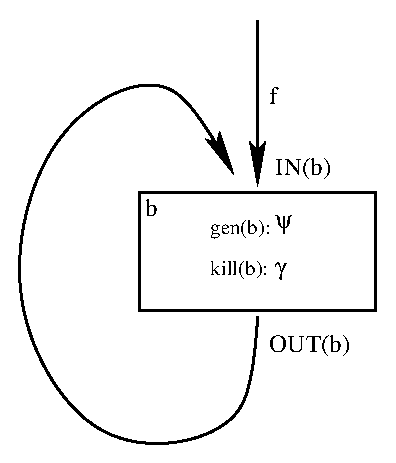
\includegraphics[scale=1]{Figure/figure_1} 
}
&
\scalebox{.7} {
\begin{tabular}{|c|c|c|}
\hline
Iteration & IN(b) & OUT(b) \\ \hline
\hline
$1$ & $f$									& $(f \wedge \KillSym) \vee \GenSym$ \\ \hline 
$2$ & $f \vee ((f \wedge \KillSym) \vee \GenSym)$	& 
			$\begin{array}{cl}
				& ((f \vee ((f \wedge \KillSym) \vee \GenSym)) \wedge \KillSym) \vee \GenSym \\
			 	=& (((f \vee (f \wedge \KillSym)) \vee \GenSym) \wedge \KillSym) \vee \GenSym \\
			 	=& ((f \vee \GenSym) \wedge \KillSym) \vee \GenSym \\
			 	=& (f \vee \GenSym \vee \GenSym) \wedge (\KillSym \vee \GenSym) \\
			 	=& (f \vee \GenSym) \wedge (\KillSym \vee \GenSym) \\
			 	=& (f \wedge \KillSym) \vee \GenSym \\
			\end{array}$ \\ \hline 
$3$ & $f \vee ((f \wedge \KillSym) \vee \GenSym)$	& $(f \wedge \KillSym) \vee \GenSym$ \\ \hline
\end{tabular}
}
\\ \\
 \footnotesize (a) Data Flow & \footnotesize (b) Data flow values per iteration \\
\end{tabular}
\label{fig:flowdiag}
\caption{The termination of computation of boolean functions}
\end{figure}


%%%%%%%%%%%%%%%%%%%%%%%%%%%%%%%%%%%%%%%%%%%%%%%%%%%%%
\section{Storage Requirement}
%%%%%%%%%%%%%%%%%%%%%%%%%%%%%%%%%%%%%%%%%%%%%%%%%%%%%

The memory requirement of our analysis consists of the
    storage space for the matrices ( $D_F$ and
    $I_F$ ) and the boolean functions.  Let $n \in
    \nat$ denotes the cardinality of the set $\heap$ at a
    program point. Obviously $n$ is bounded by the total
    number of pointer variables in the program. Let $m \in
    \nat$ denotes the maximum number of possible distinct
    pointer fields emanating from a heap directed pointer,
    which is again a bounded quantity. Between two pointer,
    for each field, we only use: (a) the ($k$-limited) count
    of the number of indirect paths starting at that given
    field, and (b) if there is a direct path using that
    field, the storage requirement for the matrices is
    bounded as:
\begin{eqnarray*}
\mbox{Space requirement for } D_F &:&  O(n^{2}* m) \\
\mbox{Space requirement for } I_F &:& O(n^{2} * m^2)
\end{eqnarray*}

The boolean functions at each program point are stored in an
expression tree.  As can be seen from the equations for the
boolean functions, the height and width of the expression
tree for a function is polynomial in the number of pointer
instructions in the program. By carefully reusing the trees
for the subexpressions in an expression, it is possible to
store the boolean functions efficiently.


%% \cmt{
%% \begin{figure}[t]
%% \centering
%% \begin{tabular}{@{}lc@{}}
%% {\small\tt
%%       \begin{tabular}[b]{l}
%%         S1. s$\rightarrow$f1 = p; \\
%%         S2. q$\rightarrow$f2 = s; 
%%       \end{tabular}
%%     } & 
\includegraphics[scale=2]{Figure/figure_17} \\ 
%% \footnotesize
%% (a) A code fragment & 
%% \footnotesize (b) Expression tree storing the boolean
%% functions \\ 
%% & \footnotesize generated after {\tt S2}. \\
%%   \end{tabular}
%%   \caption{Scheme to store the boolean functions generated at
%%     each program point}
%% \label{fig:performance_storage}
%% \end{figure}
%% }

%\chapter{Comparison with Field Insensitive Approach}\label{ch:Comparison}
\chapter{Comparison with Other Approaches}\label{ch:Comparison}

For comparison purpose the test-cases must involve shape
transitions like Cycle to DAG, Cycle to Tree, and DAG to
Tree. The transition like Tree to DAG, DAG to Cycle, or Tree
to Cycle are not of much importance as these can be detected
by any of the field insensitive approaches. Following are the
cases that meet our requirement and better demonstrate the
accuracy of our analysis as compared to field insensitive
analysis (like Ghiya et. al.~\cite{Ghiya96}).

%%%%%%%%%%%%%%%%%%%%%%%%%%%%%%%%%%%%%%%%%%%%%%%%%%%%%%%%%
\section{Comparison with Ghiya et. al.~\cite{Ghiya96}}
%%%%%%%%%%%%%%%%%%%%%%%%%%%%%%%%%%%%%%%%%%%%%%%%%%%%%%%%%

\newcommand{\nO}{\mbox{\tt n1}}
\newcommand{\nT}{\mbox{\tt n2}}
\newcommand{\myt}{\mbox{\tt t}}
\newcommand{\T}{\mbox{\tt T}}
\newcommand{\myL}{\mbox{\tt L}}
\newcommand{\R}{\mbox{\tt R}}

%%%%%%%%%%%%%%%%%%%%%%%%%%%%%%%%%%%%%%%%%%%%%%%%%%%%%
\subsection{Inserting an internal node in a singly linked list.}
%%%%%%%%%%%%%%%%%%%%%%%%%%%%%%%%%%%%%%%%%%%%%%%%%%%%%
Consider the code fragment Fig.~\ref{fig:benchmark_1}(a) that
is a simplified version of insertion of an internal node in a
linked list.  Field insensitive approach like that of Ghiya
et.~al.~\cite{Ghiya96} cannot detect the kill information due
to the change of the field $f$ of {\tt \p} at {\tt S4} and
finds {\tt \p} to have an additional path to $\q$ via {\tt
  \myr} (which is now actually the only path). So they report
the shape attribute of {\tt \p} as DAG.
Figure~\ref{fig:benchmark_1}(c) shows the $D_F$ and $I_F$ matrices
corresponding to our analysis at each program point.
Consider the following boolean function generated after {\tt
  S4} using our approach.
\begin{eqnarray*}
  \p_{\subD} &=&   (f_{\p\q} \wedge (\num{I_F[\p\q]} > 1)) 
  \vee  (f_{\p\myr} \wedge (\num{I_F[\p\myr]} > 1)), \\
  f_{\p\myr} &=& \true, \qquad\qquad  f_{\p\q} = \false \enspace. 
\end{eqnarray*}
After {\tt S4}, the condition $\num{I_F[\p,\myr]} > 1$ become
\false\ and $\p_{\subD}$ will get evaluated to \false, and
thus correctly detects the shape attribute of {\tt \p} as
tree.

\begin{figure}
\centering
\scalebox{0.80}{
\begin{tabular}{@{}c@{}}
\begin{tabular}{@{}cc@{}}
  {\small\tt
    \begin{tabular}[b]{l}
      S1. \p$\rightarrow$f = \q; \\
      S2. \myr = malloc(); \\
      S3. \myr$\rightarrow$f = q;  \\
      S4. \p$\rightarrow$f = \myr;  
    \end{tabular}
  } &
  \scalebox{0.80}{
    \begin{tabular}[b]{|c||c|c|c|}
      \hline
          {\bf After} & Actual Shape & Field Insensitive
          Analysis & Field Sensitive Analysis \\ 
          \hline \hline
	  {\tt S1}       & Tree		  & Tree    & Tree \\ \hline
	  {\tt S2}       & Tree		  & Tree    & Tree \\ \hline
	  {\tt S3}       & Tree		  & Tree    & Tree \\ \hline
	  {\tt S4}       & Tree		  & DAG(at {\tt \p})    & Tree \\ \hline
    \end{tabular}
  } \\
  \footnotesize (a) A code fragment & \footnotesize (b) Shape Inference \\ \\
 \end{tabular} \\ 
  \scalebox{0.80}{
\begin{tabular}[b]{|l@{}|@{}c@{}|@{}c@{}|} \hline
 {\bf After} & $D_F$ & $I_F$ \\ 
 {\bf Stmt} & & \\ \hline

{\tt S1} & 
\begin{tabular}{|p{3mm}|p{12mm}p{12mm}p{12mm}|} \hline 
            & $\p$  		& $\myr$ 		& $\q$ 	 \\ \hline
  $\p$ 	& $\emptyset$	& $\emptyset$	& $\{\fieldD{f}{}\}$ \\ \hline
  $\myr$ 	& $\emptyset$	& $\emptyset$	& $\emptyset$	\\ \hline
  $\q$ 		& $\emptyset$	& $\emptyset$	& $\emptyset$	\\ \hline
\end{tabular}
 &
\begin{tabular}{|p{3mm}|p{28mm}p{28mm}p{28mm}|} \hline 
            & $\p$  		& $\myr$ 		& $\q$ 	 \\ \hline
  $\p$ 	& $\emptyset$	& $\emptyset$	& $\{(\fieldD{f}{}, \epsilon)\}$ \\ \hline
  $\myr$ 	& $\emptyset$	& $\emptyset$	& $\emptyset$	\\ \hline
  $\q$ 		& $\{(\epsilon, \fieldD{f}{})$	& $\emptyset$	& $\emptyset$	\\ \hline
\end{tabular} \\ \hline

{\tt S2} & 
\begin{tabular}{|p{3mm}|p{12mm}p{12mm}p{12mm}|} \hline 
            & $\p$  		& $\myr$ 		& $\q$ 	 \\ \hline
  $\p$ 	& $\emptyset$	& $\emptyset$	& $\{\fieldD{f}{}\}$ \\ \hline
  $\myr$ 	& $\emptyset$	& $\{\epsilon\}$	& $\emptyset$	\\ \hline
  $\q$ 		& $\emptyset$	& $\emptyset$	& $\emptyset$	\\ \hline
\end{tabular}
 &
\begin{tabular}{|p{3mm}|p{28mm}p{28mm}p{28mm}|} \hline 
            & $\p$  		& $\myr$ 		& $\q$ 	 \\ \hline
  $\p$ 	& $\emptyset$	& $\emptyset$	& $\{(\fieldD{f}{}, \epsilon)\}$ \\ \hline
  $\myr$ 	& $\emptyset$	& $\{(\epsilon, \epsilon)\}$	& $\emptyset$	\\ \hline
  $\q$ 		& $\{(\epsilon, \fieldD{f}{})$	& $\emptyset$	& $\emptyset$	\\ \hline
\end{tabular} \\ \hline

{\tt S3} & 
\begin{tabular}{|p{3mm}|p{12mm}p{12mm}p{12mm}|} \hline 
            & $\p$  		& $\myr$ 		& $\q$ 	 \\ \hline
  $\p$ 	& $\emptyset$	& $\emptyset$	& $\{\fieldD{f}{}\}$ \\ \hline
  $\myr$ 	& $\emptyset$	& $\{\epsilon\}$	& $\{\fieldD{f}{}\}$	\\ \hline
  $\q$ 		& $\emptyset$	& $\emptyset$	& $\emptyset$	\\ \hline
\end{tabular}
 &
\begin{tabular}{|p{3mm}|p{28mm}p{28mm}p{28mm}|} \hline 
            & $\p$  		& $\myr$ 		& $\q$ 	 \\ \hline
  $\p$ 	& $\emptyset$	& $\emptyset$	& $\{(\fieldD{f}{}, \epsilon)\}$ \\ \hline
  $\myr$ 	& $\emptyset$	& $\{(\epsilon, \epsilon)\}$	& $\{(\fieldD{f}{}, \epsilon)\}$	\\ \hline
  $\q$ 		& $\{(\epsilon, \fieldD{f}{})\}$	& $\{(\epsilon, \fieldD{f}{})\}$	& $\emptyset$	\\ \hline
\end{tabular} \\ \hline

{\tt S4} & 
\begin{tabular}{|p{3mm}|p{12mm}p{12mm}p{12mm}|} \hline 
            & $\p$  		& $\myr$ 		& $\q$ 	 \\ \hline
  $\p$ 	& $\emptyset$	& $\{\fieldD{f}{}\}$	& $\{\fieldI{f}{}{1}\}$ \\ \hline
  $\myr$ 	& $\emptyset$	& $\{\epsilon\}$	& $\{\fieldD{f}{}\}$	\\ \hline
  $\q$ 		& $\emptyset$	& $\emptyset$	& $\emptyset$	\\ \hline
\end{tabular}
 &
\begin{tabular}{|p{3mm}|p{28mm}p{28mm}p{28mm}|} \hline 
            & $\p$  		& $\myr$ 		& $\q$ 	 \\ \hline
  $\p$ 	& $\emptyset$	& $\{(\fieldD{f}{}, \epsilon)\}$	& $\{(\fieldI{f}{}{1}, \epsilon)\}$ \\ \hline
  $\myr$ 	& $\{(\epsilon, \fieldD{f}{})\}$	& $\{(\epsilon, \epsilon)\}$	& $\{(\fieldD{f}{}, \epsilon)\}$	\\ \hline
  $\q$ 		& $\{(\epsilon, \fieldI{f}{}{1})\}$	& $\{(\epsilon, \fieldD{f}{})\}$	& $\emptyset$	\\ \hline
\end{tabular} \\ \hline
\end{tabular} 
}  \\
  \footnotesize (c) Direction ($D_F$) and Interference ($I_F$) matrices  \\ \\
\end{tabular}}
\caption{Insertion of an internal node in a singly linked list\label{fig:benchmark_1}}
\end{figure}

%%%%%%%%%%%%%%%%%%%%%%%%%%%%%%%%%%%%%%%%%%%%%%%%%%%%%
\subsection{Swapping Two Nodes of a Singly Linked List.}
%%%%%%%%%%%%%%%%%%%%%%%%%%%%%%%%%%%%%%%%%%%%%%%%%%%%%
Consider the code fragment Fig.~\ref{fig:benchmark_2}(a)
which swaps the two pointers $p\rightarrow f$ (say $n1$) and $p\rightarrow f\rightarrow f$ (say $n2$) in a
singly linked list $L$ with link field as $f$, given the
pointer $p$. Also let $t$ be the node
following the heap object $n2$ using $f$ link. 
After {\tt S1}, a temporary Cycle is created on $\p, n1 \mbox{ and } n2$, which get destroyed
after the statement {\tt S2}. This temporary shape transition is detected by our analysis.
The table in Fig.~\ref{fig:benchmark_2}(b) shows the
comparison between the shape decision given by our approach
and the field insensitive approaches.
Consider the following boolean functions generated after {\tt
  S1} using our approach.
\begin{eqnarray*}
  n2_{\subC} &=&   (f_{n2,n1} \wedge \num{D_F[n1,n2]} \geq 1) \\ 
  n1_{\subC} &=&   (f_{n2,n1} \wedge \num{D_F[n1,n2]} \geq 1) \\ 
  \p_{\subC} &=&   (\num{D_F[p,n2]} \geq 1 \wedge f_{n2,n1} \wedge \num{D_F[n1,n2]} \geq 1) \\ 
  \p_{\subC} &=&   (\num{D_F[p,n1]} \geq 1 \wedge f_{n2,n1} \wedge \num{D_F[n1,n2]} \geq 1) \\
  f_{n2,n1} &=& \true 
\end{eqnarray*}
As depicted in Fig.~\ref{fig:benchmark_2}(c) which summarises the $D_F$ and $I_F$ matrices computed using our analysis, 
beyond {\tt S2} the condition $\num{D_F[n1,n2]} \geq 1$ becomes \false\ and thus the shape transition from Cycle 
to Tree is reported.


\begin{figure}
\centering
\scalebox{0.8}{
\begin{tabular}{@{}c@{}}
\begin{tabular}{@{}cc@{}}
  {\small\tt
    \begin{tabular}[b]{l}
      %S1. n1 = p$\rightarrow$f; \\
      %S2. n2 = n1$\rightarrow$f; \\
      %S3. t  = n2$\rightarrow$f; \\
      S1. n2$\rightarrow$f = n1; \\
      S2. n1$\rightarrow$f = t; \\
      S3. p$\rightarrow$f = n2;
    \end{tabular}
  } &
  \scalebox{0.80}{
    \begin{tabular}[b]{|c||c|c|c|}
      \hline
          {\bf After} & Actual Shape & Field Insensitive
          Analysis & Field Sensitive Analysis \\ 
          \hline \hline
         % {\tt S1}       & Tree		  & Tree                       & Tree \\ \hline
         % {\tt S2}       & Tree		  & Tree                       & Tree \\ \hline
	  %{\tt S3}       & Tree		  & Tree                       & Tree \\ \hline
	  {\tt S1}       & Cycle (at {\tt p}, {\tt n1}, {\tt n2}) 	   & Cycle (at {\tt p}, {\tt n1}, {\tt n2}) & Cycle (at {\tt p}, {\tt n1}, {\tt n2}) \\ \hline
	  {\tt S2}       & Tree		  & Cycle (at {\tt p}, {\tt n1}, {\tt n2})                       & Tree \\ \hline
	  {\tt S3}       & Tree		  & Cycle (at {\tt p}, {\tt n1}, {\tt n2})                       & Tree \\ \hline
    \end{tabular}
  } \\ 
  \footnotesize (a) A code fragment & \footnotesize (b) Shape Inference \\ \\
  \end{tabular} \\ 
  \scalebox{0.80}{
\begin{tabular}[b]{|l@{}|@{}c@{}|@{}c@{}|} \hline
 {\bf After} & $D_F$ & $I_F$ \\ 
 {\bf Stmt} & & \\ \hline
{\tt S1} & 
\begin{tabular}{|p{3mm}|p{12mm}p{12mm}p{12mm}p{12mm}|} \hline 
            & $\nO$  								& $\nT$ 				& $\p$ 			& $\myt$ \\ \hline
  $\nO$ 	& $\{\fieldI{f}{}{1}\}$						& $\{\fieldD{f}{}, \fieldI{f}{}{1}\}$	& $\{\fieldI{f}{}{1}\}$	& $\{\fieldI{f}{}{1}\}$ \\ \hline
  $\nT$ 	& $\{\fieldD{f}{}\}$						& $\{\fieldI{f}{}{1}\}$			& $\emptyset$	& $\{\fieldI{f}{}{1}\}$ \\ \hline
  $\p$ 		& $\{\fieldD{f}{}, \fieldI{f}{}{1}\}$	& $\{\fieldI{f}{}{2}\}$		& $\emptyset$	& $\{\fieldI{f}{}{2}\}$ \\ \hline
  $\myt$ 	& $\emptyset$							& $\emptyset$			& $\emptyset$	& $\emptyset$ \\ \hline
\end{tabular}
 &
\begin{tabular}{|p{3mm}|p{28mm}p{28mm}p{28mm}p{28mm}|} \hline 
			& $\nO$  											& $\nT$ 														& $\p$ 			& $\myt$ \\ \hline
	$\nO$ 	& $\{(\fieldI{f}{}{1}, \epsilon)\}$					& $\{(\fieldD{f}{}, \epsilon), (\epsilon, \fieldD{f}{})\}$		& $\{(\epsilon, \fieldD{f}{})\}$	& $\emptyset$ \\ \hline
  $\nT$ 	& $\{(\fieldD{f}{}, \epsilon), (\epsilon, \fieldD{f}{})\}$	& $\{(\fieldI{f}{}{1}, \epsilon)\}$						& $\{(\epsilon, \fieldI{f}{}{1})\}$	& $\emptyset$ \\ \hline
  $\p$ 		& $\{(\fieldD{f}{}, \epsilon)\}$	& $\{(\fieldI{f}{}{1}, \epsilon)\}$	& $\emptyset$	& $\emptyset$ \\ \hline
  $\myt$ 	& $\emptyset$						& $\emptyset$						& $\emptyset$	& $\emptyset$ \\ \hline
\end{tabular} \\ \hline

{\tt S2} & 
\begin{tabular}{|p{3mm}|p{12mm}p{12mm}p{12mm}p{12mm}|} \hline
            & $\nO$  								& $\nT$ 				& $\p$ 			& $\myt$ \\ \hline
  $\nO$ 	& $\emptyset$							& $\emptyset$			& $\emptyset$	& $\{\fieldD{f}\}$ \\ \hline
  $\nT$ 	& $\{\fieldD{f}{}\}$					& $\{\fieldI{f}{}{1}\}$			& $\emptyset$	& $\{\fieldI{f}{}{1}\}$ \\ \hline
  $\p$ 		& $\{\fieldD{f}{}, \fieldI{f}{}{1}\}$	& $\{\fieldD{f}{}, \fieldI{f}{}{3}\}$			& $\emptyset$	& $\fieldI{f}{}{2}$ \\ \hline
  $\myt$ 	& $\emptyset$							& $\emptyset$			& $\emptyset$	& $\emptyset$ \\ \hline
\end{tabular}
 &
\begin{tabular}{|p{3mm}|p{28mm}p{28mm}p{28mm}p{28mm}|} \hline
			& $\nO$  							& $\nT$ 							& $\p$ 			& $\myt$ \\ \hline
			 $\nO$ 	& $\emptyset$						& $\{(\epsilon, \fieldD{f}{})\}$	& $\{(\epsilon, \fieldD{f}{})\}$	& $\{(\fieldD{f}{},\epsilon)\}$ \\ \hline
  $\nT$ 	& $\{(\fieldD{f}{}, \epsilon)\}$	& $\emptyset$						& $\{(\epsilon, \fieldI{f}{}{1})\}$	& $\{(\fieldI{f}{}{1}, \epsilon)\}$ \\ \hline
  $\p$ 		& $\{(\fieldD{f}{}, \epsilon)\}$	& $\{(\fieldI{f}{}{1}, \epsilon)\}$	& $\emptyset$	& $\{(\fieldI{f}{}{1}, \epsilon)\}$ \\ \hline
  $\myt$ 	& $\{(\epsilon, \fieldD{f}{})\}$		& $\{(\epsilon, \fieldI{f}{}{1})\}$		& $\{(\epsilon, \fieldI{f}{}{1})\}$	& $\emptyset$ \\ \hline
\end{tabular} \\ \hline

{\tt S3} & 
\begin{tabular}{|p{3mm}|p{12mm}p{12mm}p{12mm}p{12mm}|} \hline
            & $\nO$  								& $\nT$ 				& $\p$ 			& $\myt$ \\ \hline
  $\nO$ 	& $\emptyset$							& $\emptyset$			& $\emptyset$	& $\{\fieldD{f}{}\}$ \\ \hline
  $\nT$ 	& $\{\fieldD{f}{}\}$					& $\{\fieldI{f}{}{1}\}$			& $\emptyset$	& $\{\fieldI{f}{}{1}\}$ \\ \hline
  $\p$ 		& $\{\fieldI{f}{}{1}\}$					& $\{\fieldD{f}{}, \fieldI{f}{}{1}\}$	& $\emptyset$	& $\{\fieldI{f}{}{1}\}$ \\ \hline
  $\myt$ 	& $\emptyset$							& $\emptyset$			& $\emptyset$	& $\emptyset$ \\ \hline
\end{tabular}
 &
\begin{tabular}{|p{3mm}|p{28mm}p{28mm}p{28mm}p{28mm}|} \hline
			& $\nO$  							& $\nT$ 							& $\p$ 			& $\myt$ \\ \hline
			 $\nO$ 	& $\emptyset$						& $\{(\epsilon, \fieldD{f}{})\}$	& $\{(\epsilon, \fieldI{f}{}{1})\}$	& $\{(\fieldD{f}{},\epsilon)\}$ \\ \hline
  $\nT$ 	& $\{(\fieldD{f}{}, \epsilon)\}$	& $\emptyset$						& $\{(\epsilon, \fieldD{f}{})\}$	& $\{(\fieldI{f}{}{1}, \epsilon)\}$ \\ \hline
  $\p$ 		& $\{(\fieldI{f}{}{1}, \epsilon)\}$	& $\{(\fieldD{f}{}, \epsilon)\}$	& $\emptyset$	& $\{(\fieldI{f}{}{1}, \epsilon)\}$ \\ \hline
  $\myt$ 	& $\{(\epsilon, \fieldD{f}{})\}$		& $\{(\epsilon, \fieldI{f}{}{1})\}$		& $\{(\epsilon, \fieldI{f}{}{1})\}$	& $\emptyset$ \\ \hline
\end{tabular}  \\ \hline
\end{tabular} 
}  \\
  \footnotesize (c) Direction ($D_F$) and Interference ($I_F$) matrices  \\ \\
\end{tabular}}
\caption{Swapping two nodes of a singly linked list\label{fig:benchmark_2}}
\end{figure}



%%{\tt S1} & 
%%\begin{tabular}{|p{3mm}|p{12mm}p{12mm}p{12mm}p{12mm}|} \hline 
%%            & $\nO$  		& $\nT$ 		& $\p$ 			& $\myt$ \\ \hline
 %% $\nO$ 	& $\emptyset$	& $\emptyset$	& $\emptyset$	& $\emptyset$ \\ \hline
%%  $\nT$ 	& $\emptyset$	& $\emptyset$	& $\emptyset$	& $\emptyset$ \\ \hline
%%  $\p$ 		& $\{\fieldD{f}{}\}$	& $\emptyset$	& $\emptyset$	& $\emptyset$ \\ \hline
%%  $\myt$ 		& $\emptyset$	& $\emptyset$	& $\emptyset$	& $\emptyset$ \\ \hline
%%\end{tabular}
%% &
%%\begin{tabular}{|p{3mm}|p{28mm}p{28mm}p{28mm}p{28mm}|} \hline 
%%			& $\nO$  						& $\nT$ 		& $\p$ 			& $\myt$ \\ \hline
%%  $\nO$ 	& $\emptyset$					& $\emptyset$	& $\{(\epsilon, \fieldD{f}{})\}$	& $\emptyset$ \\ \hline
%%  $\nT$ 	& $\emptyset$					& $\emptyset$	& $\emptyset$	& $\emptyset$ \\ \hline
%%  $\p$ 		& $\{(\fieldD{f}{}, \epsilon)\}$	& $\emptyset$	& $\emptyset$	& $\emptyset$ \\ \hline
%%  $\myt$ 	& $\emptyset$					& $\emptyset$	& $\emptyset$	& $\emptyset$ \\ \hline
%%\end{tabular} \\ \hline
%%
%%{\tt S2} & 
%%\begin{tabular}{|p{3mm}|p{12mm}p{12mm}p{12mm}p{12mm}|} \hline 
%%            & $\nO$  				& $\nT$ 				& $\p$ 			& $\myt$ \\ \hline
 %%%% $\nO$ 	& $\emptyset$			& $\{\fieldD{f}{}\}$	& $\emptyset$	& $\emptyset$ \\ \hline
%%  $\nT$ 	& $\emptyset$			& $\emptyset$			& $\emptyset$	& $\emptyset$ \\ \hline
%%  $\p$ 		& $\{\fieldD{f}{}\}$	& $\fieldI{f}{}{1}$		& $\emptyset$	& $\emptyset$ \\ \hline
 %%%% $\myt$ 	& $\emptyset$			& $\emptyset$			& $\emptyset$	& $\emptyset$ \\ \hline
%%end{tabular}
%% &
%%\begin{tabular}{|p{3mm}|p{28mm}p{28mm}p{28mm}p{28mm}|} \hline 
%%			& $\nO$  						& $\nT$ 							& $\p$ 			& $\myt$ \\ \hline
%%  $\nO$ 	& $\emptyset$					& $\{(\fieldD{f}{}, \epsilon)\}$		& $\{(\epsilon, \fieldD{f}{})\}$	& $\emptyset$ \\ \hline
%%  $\nT$ 	& $\{(\epsilon, \fieldD{f}{})\}$					& $\emptyset$		& $\{(\epsilon, \fieldI{f}{}{1})\}$	& $\emptyset$ \\ \hline
%%  $\p$ 		& $\{(\fieldD{f}{}, \epsilon)\}$& $\{(\fieldI{f}{}{1}, \epsilon)\}$	& $\emptyset$	& $\emptyset$ \\ \hline
%%  $\myt$ 	& $\emptyset$					& $\emptyset$						& $\emptyset$	& $\emptyset$ \\ \hline
%%\end{tabular} \\ \hline

%%{\tt S3} & 
%%\begin{tabular}{|p{3mm}|p{12mm}p{12mm}p{12mm}p{12mm}|} \hline 
%%            & $\nO$  				& $\nT$ 				& $\p$ 			& $\myt$ \\ \hline
%%  $\nO$ 	& $\emptyset$			& $\{\fieldD{f}{}\}$	& $\emptyset$	& $\{\fieldI{f}{}{1}\}$ \\ \hline
%%  $\nT$ 	& $\emptyset$			& $\emptyset$			& $\emptyset$	& $\{\fieldD{f}{}\}$ \\ \hline
%%  $\p$ 		& $\{\fieldD{f}{}\}$	& $\fieldI{f}{}{1}$		& $\emptyset$	& $\{\fieldI{f}{}{1}\}$ \\ \hline
%%  $\myt$ 	& $\emptyset$			& $\emptyset$			& $\emptyset$	& $\emptyset$ \\ \hline
%%\end{tabular}
%% &
%%\begin{tabular}{|p{3mm}|p{28mm}p{28mm}p{28mm}p{28mm}|} \hline 
%%			& $\nO$  						& $\nT$ 							& $\p$ 			& $\myt$ \\ \hline
%%  $\nO$ 	& $\emptyset$					& $\{(\fieldD{f}{}, \epsilon)\}$		& $\{(\epsilon, \fieldD{f}{})\}$	& $\{(\fieldI{f}{}{1}, \epsilon)\}$ \\ \hline
%%  $\nT$ 	& $\{(\epsilon, \fieldD{f}{})\}$					& $\emptyset$		& $\{(\epsilon, \fieldI{f}{}{1})\}$	& $\{(\fieldD{f}{}, \epsilon)\}$ \\ \hline
 %% $\p$ 		& $\{(\fieldD{f}{}, \epsilon)\}$	& $\{(\fieldI{f}{}{1}, \epsilon)\}$	& $\emptyset$	& $\{(\fieldI{f}{}{1}, \epsilon)\}$ \\ \hline
%%  $\myt$ 	& $\{(\epsilon, \fieldI{f}{}{1})\}$					& $\{(\epsilon, \fieldD{f}{})\}$						& $\{(\epsilon, \fieldI{f}{}{1})\}$	& $\emptyset$ \\ \hline
%%\end{tabular} \\ \hline


%%%%%%%%%%%%%%%%%%%%%%%%%%%%%%%%%%%%%%%%%%%%%%%%%%%%%
\subsection{Recursively Swapping Binary Tree.}
%%%%%%%%%%%%%%%%%%%%%%%%%%%%%%%%%%%%%%%%%%%%%%%%%%%%%
Consider the code fragment Fig.~\ref{fig:benchmark_3}(a)
which creates a mirror image of a binary tree rooted at
$T$. While swapping the left and right sub-tree a temporary
DAG is created (after statement {\tt S5}), which gets
destroyed after the very next statement {\tt S6}.
Consider the following boolean functions generated after {\tt
  S5} using our approach.
\begin{eqnarray*}
  T_{\subD} &=&   (left_{T,R} \wedge \num{I_F[T,R]} > 1) \\ 
  left_{T,R} &=& \true 
\end{eqnarray*}

Figure~\ref{fig:benchmark_3}(c) shows the $D_F$ and $I_F$ matrices
corresponding to our analysis at each program point. Due to
the inclusion of the approximation (\upath) for the statements
{\tt S1} and {\tt S2}, the condition $\num{I_F[T,R]} > 1$  still holds 
beyond {\tt S6} and thus the analysis reports shape of $T$ as DAG, which is actually a Tree. 
Considering the fact that shape attribute of
$T$ is a Tree, and thus statements {\tt S1} and {\tt S2} must include
just one path between $T$ and $L$ or $T$ and $R$, we obtain
Figure~\ref{fig:benchmark_3}(d) which shows the  refined $D_F$ and $I_F$ matrices at each program
point, using which we can infer the shape of $T$ after {\tt S6} as Tree because the condition $\num{I_F[T,R]} > 1$ 
evaluated to \false\ after {S6}. Figure ~\ref{fig:benchmark_3}(b) shows the shape transition at each program 
point using this refined analysis.


\begin{figure}
\centering
\scalebox{0.80}{
\begin{tabular}{@{}c@{}}
\begin{tabular}{@{}cc@{}}
  {\small \tt
    \begin{tabular}[b]{l}
      mirror(tree T) \{ \\
      S1.    L  = T->left; \\
      S2.    R = T->right; \\
      S3.    mirror(L); \\
      S4.    mirror(R); \\
      S5.    T->left = R; \\
      S6.    T->right = L; \\
      \}  
    \end{tabular}
  } &
  \scalebox{0.80}{
    \begin{tabular}[b]{|c||c|c|c|}
      \hline
          {\bf After} & Actual Shape & Field Insensitive
          Analysis & Field Sensitive Analysis \\ 
          \hline \hline
	  {\tt S1}       & Tree		  & Tree    & Tree \\ \hline
	  {\tt S2}       & Tree		  & Tree    & Tree \\ \hline
	  {\tt S5}       & Dag (at T)	  & Dag (at T)    & Dag (at T) \\ \hline
	  {\tt S6}       & Tree		  & Dag (at T)    & Tree \\ \hline
    \end{tabular}
  } \\
  \footnotesize (a) A code fragment & \footnotesize (b) Shape Inference \\ \\
  \end{tabular} \\
  \scalebox{0.80}{
\begin{tabular}[b]{|l@{}|@{}c@{}|@{}c@{}|} \hline
 {\bf After} & $D_F$ & $I_F$ \\ 
 {\bf Stmt} & & \\ \hline

{\tt S1} & 
\begin{tabular}{|p{3mm}|p{22mm}p{22mm}p{22mm}|} \hline 
            & $\T$  		& $\myL$ 		& $\R$ 	 \\ \hline
  $\T$ 	& $\emptyset$	& $\{\fieldD{l}{}\} \cup \upath$	& $\emptyset$ \\ \hline
  $\myL$ 	& $\emptyset$	& $\emptyset$	& $\emptyset$	\\ \hline
  $\R$ 		& $\emptyset$	& $\emptyset$	& $\emptyset$	\\ \hline
\end{tabular}
 &
\begin{tabular}{|p{3mm}|p{35mm}p{35mm}p{35mm}|} \hline 
            & $\T$  		& $\myL$ 		& $\R$ 	 \\ \hline
  $\T$ 	& $\emptyset$	& $(\{\fieldD{l}{}\} \cup \upath) \times \{\epsilon\}$	& $\emptyset$ \\ \hline
  $\myL$ 	& $\{\epsilon\} \times (\{\fieldD{l}{}\} \cup \upath)$	& $\emptyset$	& $\emptyset$	\\ \hline
  $\R$ 		& $\emptyset$	& $\emptyset$	& $\emptyset$	\\ \hline
\end{tabular} \\ \hline

{\tt S2} & 
\begin{tabular}{|p{3mm}|p{22mm}p{22mm}p{22mm}|} \hline 
            & $\T$  		& $\myL$ 		& $\R$ 	 \\ \hline
  $\T$ 	& $\emptyset$	& $\{\fieldD{l}{}\} \cup \upath$	& $\{\fieldD{r}{}\} \cup \upath$ \\ \hline
  $\myL$ 	& $\emptyset$	& $\emptyset$	& $\emptyset$	\\ \hline
  $\R$ 		& $\emptyset$	& $\emptyset$	& $\emptyset$	\\ \hline
\end{tabular}
 &
\begin{tabular}{|p{3mm}|p{35mm}p{35mm}p{35mm}|} \hline 
            & $\T$  		& $\myL$ 		& $\R$ 	 \\ \hline
  $\T$ 	& $\emptyset$	& $(\{\fieldD{l}{}\} \cup \upath) \times \{\epsilon\}$	& $(\{\fieldD{r}{}\} \cup \upath) \times \{\epsilon\}$ \\ \hline
  $\myL$ 	& $\{\epsilon\} \times (\{\fieldD{l}{}\} \cup \upath)$	& $\emptyset$	& $\emptyset$	\\ \hline
  $\R$ 		& $\{\epsilon\} \times (\{\fieldD{r}{}\} \cup \upath)$	& $\emptyset$	& $\emptyset$	\\ \hline
\end{tabular} \\ \hline

{\tt S5} & 
\begin{tabular}{|p{3mm}|p{22mm}p{22mm}p{22mm}|} \hline
            & $\T$  		& $\myL$ 		& $\R$ 	 \\ \hline
  $\T$ 		& $\emptyset$	& $\upath$	& $\{\fieldD{r}{}, \fieldD{l}{}\} \cup \upath$ \\ \hline
  $\myL$ 	& $\emptyset$	& $\emptyset$	& $\emptyset$	\\ \hline
  $\R$ 		& $\emptyset$	& $\emptyset$	& $\emptyset$	\\ \hline
\end{tabular}
 &
\begin{tabular}{|p{3mm}|p{35mm}p{35mm}p{35mm}|} \hline 
            & $\T$  		& $\myL$ 		& $\R$ 	 \\ \hline
  $\T$ 		& $\emptyset$	& $\upath \times \{\epsilon\}$	& $(\{\fieldD{r}{}, \fieldD{l}{}\} \cup \upath) \times \{\epsilon\}$ \\ \hline
  $\myL$ 	& $\{\epsilon\} \times \upath$	& $\emptyset$	& $\emptyset$	\\ \hline
  $\R$ 		& $\{\epsilon\} \times (\{\fieldD{r}{}, \fieldD{l}{}\} \cup \upath)$	& $\emptyset$	& $\emptyset$	\\ \hline
\end{tabular} \\ \hline

{\tt S6} & 
\begin{tabular}{|p{3mm}|p{22mm}p{22mm}p{22mm}|} \hline
            & $\T$  		& $\myL$ 		& $\R$ 	 \\ \hline
  $\T$ 		& $\emptyset$	& $\{\fieldD{r}{}\} \cup \upath$	& $\{\fieldD{l}{}\} \cup \upath$ \\ \hline
  $\myL$ 	& $\emptyset$	& $\emptyset$	& $\emptyset$	\\ \hline
  $\R$ 		& $\emptyset$	& $\emptyset$	& $\emptyset$	\\ \hline
\end{tabular}
 &
\begin{tabular}{|p{3mm}|p{35mm}p{35mm}p{35mm}|} \hline
            & $\T$  		& $\myL$ 		& $\R$ 	 \\ \hline
  $\T$ 		& $\emptyset$	& $(\{\fieldD{r}{}\} \cup \upath) \times \{\epsilon\}$	& $(\{\fieldD{l}{}\} \cup \upath) \times \{\epsilon\}$ \\ \hline
  $\myL$ 	& $\{\epsilon\} \times (\{\fieldD{r}{}\} \cup \upath)$	& $\emptyset$	& $\emptyset$	\\ \hline
  $\R$ 		& $\{\epsilon\} \times (\{\fieldD{l}{}\} \cup \upath)$	& $\emptyset$	& $\emptyset$	\\ \hline
\end{tabular} \\ \hline
\end{tabular} 
}  \\
  \footnotesize (c) Direction ($D_F$) and Interference ($I_F$) matrices  \\ \\
  \scalebox{0.80}{
\begin{tabular}[b]{|l@{}|@{}c@{}|@{}c@{}|} \hline
 {\bf After} & $D_F$ & $I_F$ \\ 
 {\bf Stmt} & & \\ \hline

{\tt S1} & 
\begin{tabular}{|p{3mm}|p{12mm}p{12mm}p{12mm}|} \hline 
            & $\T$  		& $\myL$ 		& $\R$ 	 \\ \hline
  $\T$ 	& $\emptyset$	& $\{\fieldD{l}{}\}$	& $\emptyset$ \\ \hline
  $\myL$ 	& $\emptyset$	& $\emptyset$	& $\emptyset$	\\ \hline
  $\R$ 		& $\emptyset$	& $\emptyset$	& $\emptyset$	\\ \hline
\end{tabular}
 &
\begin{tabular}{|p{3mm}|p{28mm}p{28mm}p{28mm}|} \hline 
            & $\T$  		& $\myL$ 		& $\R$ 	 \\ \hline
  $\T$ 	& $\emptyset$	& $\{(\fieldD{l}{}, \epsilon)\}$	& $\emptyset$ \\ \hline
  $\myL$ 	& $\{(\epsilon, \fieldD{l}{})\}$	& $\emptyset$	& $\emptyset$	\\ \hline
  $\R$ 		& $\emptyset$	& $\emptyset$	& $\emptyset$	\\ \hline
\end{tabular} \\ \hline

{\tt S2} & 
\begin{tabular}{|p{3mm}|p{12mm}p{12mm}p{12mm}|} \hline 
            & $\T$  		& $\myL$ 		& $\R$ 	 \\ \hline
  $\T$ 	& $\emptyset$	& $\{\fieldD{l}{}\}$	& $\{\fieldD{r}{}\}$ \\ \hline
  $\myL$ 	& $\emptyset$	& $\emptyset$	& $\emptyset$	\\ \hline
  $\R$ 		& $\emptyset$	& $\emptyset$	& $\emptyset$	\\ \hline
\end{tabular}
 &
\begin{tabular}{|p{3mm}|p{28mm}p{28mm}p{28mm}|} \hline 
            & $\T$  		& $\myL$ 		& $\R$ 	 \\ \hline
  $\T$ 	& $\emptyset$	& $\{(\fieldD{l}{}, \epsilon)\}$	& $\{(\fieldD{r}{}, \epsilon)\}$ \\ \hline
  $\myL$ 	& $\{(\epsilon, \fieldD{l}{})\}$	& $\emptyset$	& $\emptyset$	\\ \hline
  $\R$ 		& $\{(\epsilon, \fieldD{r}{})\}$	& $\emptyset$	& $\emptyset$	\\ \hline
\end{tabular} \\ \hline

{\tt S5} & 
\begin{tabular}{|p{3mm}|p{12mm}p{12mm}p{12mm}|} \hline
            & $\T$  		& $\myL$ 		& $\R$ 	 \\ \hline
  $\T$ 		& $\emptyset$	& $\emptyset$	& $\{\fieldD{r}{}, \fieldD{l}{}\}$ \\ \hline
  $\myL$ 	& $\emptyset$	& $\emptyset$	& $\emptyset$	\\ \hline
  $\R$ 		& $\emptyset$	& $\emptyset$	& $\emptyset$	\\ \hline
\end{tabular}
 &
\begin{tabular}{|p{3mm}|p{28mm}p{28mm}p{28mm}|} \hline 
            & $\T$  		& $\myL$ 		& $\R$ 	 \\ \hline
  $\T$ 		& $\emptyset$	& $\emptyset$	& $\{(\fieldD{r}{}, \epsilon), (\fieldD{l}{}, \epsilon)\}$ \\ \hline
  $\myL$ 	& $\emptyset$	& $\emptyset$	& $\emptyset$	\\ \hline
  $\R$ 		& $\{(\epsilon, \fieldD{r}{}), (\epsilon, \fieldD{l}{})\}$	& $\emptyset$	& $\emptyset$	\\ \hline
\end{tabular} \\ \hline

{\tt S6} & 
\begin{tabular}{|p{3mm}|p{12mm}p{12mm}p{12mm}|} \hline
            & $\T$  		& $\myL$ 		& $\R$ 	 \\ \hline
  $\T$ 		& $\emptyset$	& $\{\fieldD{r}{}\}$	& $\{\fieldD{l}{}\}$ \\ \hline
  $\myL$ 	& $\emptyset$	& $\emptyset$	& $\emptyset$	\\ \hline
  $\R$ 		& $\emptyset$	& $\emptyset$	& $\emptyset$	\\ \hline
\end{tabular}
 &
\begin{tabular}{|p{3mm}|p{28mm}p{28mm}p{28mm}|} \hline
            & $\T$  		& $\myL$ 		& $\R$ 	 \\ \hline
  $\T$ 		& $\emptyset$	& $\{(\fieldD{r}{}, \epsilon)\}$	& $\{(\fieldD{l}{}, \epsilon)\}$ \\ \hline
  $\myL$ 	& $\{(\epsilon, \fieldD{r}{})\}$	& $\emptyset$	& $\emptyset$	\\ \hline
  $\R$ 		& $\{(\epsilon, \fieldD{l}{})\}$	& $\emptyset$	& $\emptyset$	\\ \hline
\end{tabular} \\ \hline
\end{tabular} 
}  \\
  \footnotesize (d) Refined Direction ($D_F$) and Interference ($I_F$) matrices  \\ \\
\end{tabular}}
\caption{Computing mirror image of a  binary tree. ``$l$'' and ``$r$'' denotes respectively the left and right fields of tree.\label{fig:benchmark_3}}
\end{figure}


%%%%%%%%%%%%%%%%%%%%%%%%%%%%%%%%%%%%%%%%%%%%%%%%%%%%%%%%%
\section{Comparison with Marron et. al.~\cite{marron06static}}
%%%%%%%%%%%%%%%%%%%%%%%%%%%%%%%%%%%%%%%%%%%%%%%%%%%%%%%%%

Using the property as mentioned in Appendix B, we inferred the shape of the data structure corresponding to 
each region for the test-cases that we have chosen, and concluded that their shape inferencing comply exactly with the actual
shapes that should be reported.

To eliminate the state explosion that is possible with refinement, they apply refinement to only those 
cases where there exist a unique way of materializing new nodes. This limits the amount of precision 
that can be achieved as there exists cases where refinement into  multiple possibilities is needed to get results with the
desired accuracy.    

% \section{Conclusion}

In this report we have suggested several enhancements to Sandeep's work on Field Sensitive analysis
which ensure the correctness and increase the accuracy of the analysis.
Now after these changes the analysis is better than Ghiya's work in all those unit test cases described. 
We have also introduced a new analysis called subset based analysis which infers shape based on the subset of fields actually accessed inside
a function. This helps us inferring information like a function is traversing/accessing a tree substructure of a cyclic data structure. 
We also proposed a shape sensitive inter procedural
analysis which is in mid way of context sensitive and context insensitive analysis and could possibly balance the memory consumption and 
preciseness at the same time. We have also performed various 
optimizations with the aim of decreasing the memory consumption and time for completion.
The testing strategy used is exhaustive and has helped a lot in identifying the cases of safe and incorrect results.

There are some benchmarks where the results are not as good as Ghiya's, these are due to the
summarization of heap nodes due to the dummy statement. In the future we plan to work on
this issue.
The analysis has concerns over the amount of memory it takes even after the optimizations performed. We want
to address this concern by representing boolean equations in much efficient way. 
% The callstring approach is using
% more memory for this analysis, so we plan to find out some other context sensitive analysis which is
% memory efficient.

% \section{Future Work}
% Representation of boolean equations in a memory efficient
% Better memory efficient Context sensitive analysis
% Extend this for arrays of pointers



\appendix
%%%%%%%%%%%%%%%%%%%%%%%%%%%%%%%%%%%%%%%%%%%%%%%%%%%%%%%%%%%%%%%%%%%%%%
\chapter[Analysis of Ghiya et. al.~\cite{Ghiya96}]{Analysis of Ghiya et. al.~\cite{Ghiya96}\footnote{The contents of this section are borrowed from ~\cite{Ghiya96}}}
%%%%%%%%%%%%%%%%%%%%%%%%%%%%%%%%%%%%%%%%%%%%%%%%%%%%%%%%%%%%%%%%%%%%%%
Most of the definitions and technical terms used in this chapter are borrowed from the aforementioned paper.
The proposed shape analysis composed of three store-less
abstractions that are computed together at each program point.
For each heap directed pointer they approximated the attribute
shape and for each pair of heap directed pointers they approximated the 
direction and interference relationships between them. These three abstractions 
are defined formally as follows:

\begin{definition}
Given any heap-directed pointer $p$, the shape attribute p.shape is Tree, 
if in the data structure accessible from p there is a unique (possibly empty) access path 
between any two nodes (heap objects) belonging to it. It is considered to be DAG (directed acyclic graph), 
if there can be more than one path between any two nodes in this data structure, 
but there is no path from a node to itself (i. e, it is acyclic). 
If the data structure contains a node having a path to itself, p.shape is considered to be Cycle.
Note that as lists are special case of tree data structures, their shape is also considered as Tree.
\end{definition}

\begin{definition}
Given two heap directed pointers $p$ and $q$, the direction matrix $D$ captures the following 
relationships between them:
\begin{itemize}
\item $D[p,q] = 1 : $ An access path possibly exists in the heap, from the heap object pointed to by $p$,
to the heap object pointed to by $q$. In this case we simply say that the pointer $p$ has a path to 
pointer $q$.
\item $D[p,q] = 0 : $ No access path exists from the heap object pointed to by $p$ to the heap object pointed to by $q$. 
\end{itemize}
\end{definition}

\begin{definition}
Given two heap directed pointers $p$ and $q$, the direction matrix $I$ captures the following 
relationships between them:
\begin{itemize}
\item $I[p,q] = 1 : $ A common heap object can be possibly accessed starting from pointers $p$ and $q$.
In this case we state that pointers $p$ and $q$ can interfere.
\item $I[p,q] = 0 : $ No common heap object can be accessed starting from pointers $p$ and $q$.
In this case we state that pointers $p$ and $q$ do not interfere.
\end{itemize}
\end{definition}

Direction relationships are used to actually estimate the shape attributes, where the interference 
relationships are used for safely calculating direction relationships. 

\subsection*{Illustrative Example}

The direction and interference matrices are illustrated in Fig.~\ref{fig:relwork_1}.
Part (a) represents a heap structures at a program point, while parts (b) and (c) show the direction 
and interference matrices for it.  
\begin{figure}
\centering
\begin{tabular}{c@{$\qquad\qquad$}c}
\multicolumn{2}{c}{
\scalebox{0.80} { 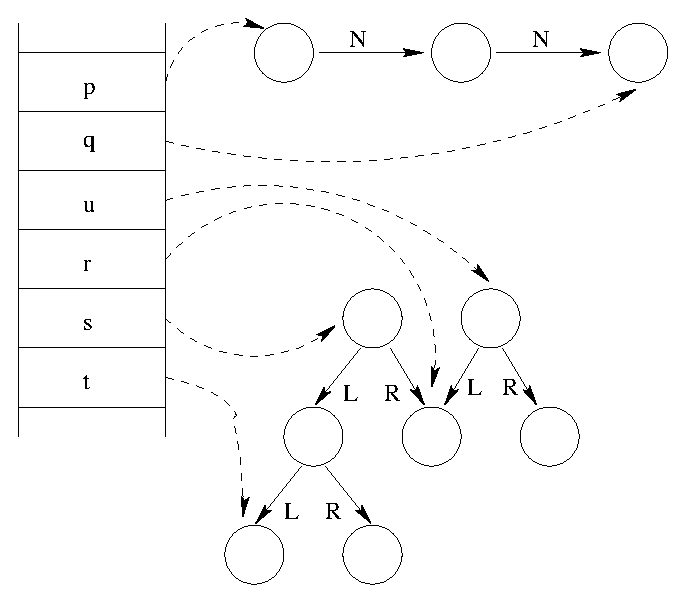
\includegraphics[scale=1]{diagrams/Appendix_2.eps}}
} \\
\multicolumn{2}{c}{
\scalebox{0.80}{ (a) Heap Structure }
} \\ \\
\scalebox{0.80} { \begin{tabular}{|c||c|c|c|c|c|c|}
\hline
$D$ & $p$ & $q$ & $r$ & $s$ & $t$ & $u$ \\ \hline \hline
$p$ & $1$ & $1$ & $0$ & $0$ & $0$ & $0$ \\ \hline 
$q$ & $0$ & $1$ & $0$ & $0$ & $0$ & $0$ \\ \hline 
$r$ & $0$ & $0$ & $1$ & $0$ & $0$ & $0$ \\ \hline 
$s$ & $0$ & $0$ & $1$ & $1$ & $1$ & $0$ \\ \hline 
$t$ & $0$ & $0$ & $0$ & $0$ & $1$ & $0$ \\ \hline 
$u$ & $0$ & $0$ & $1$ & $0$ & $0$ & $1$ \\ \hline 
\end{tabular}} 
& 
\scalebox{0.80} {\begin{tabular}{|c||c|c|c|c|c|c|}
\hline
$I$ & $p$ & $q$ & $r$ & $s$ & $t$ & $u$ \\ \hline \hline
$p$ & $1$ & $1$ & $0$ & $0$ & $0$ & $0$ \\ \hline 
$q$ & $1$ & $1$ & $0$ & $0$ & $0$ & $0$ \\ \hline 
$r$ & $0$ & $0$ & $1$ & $1$ & $0$ & $1$ \\ \hline 
$s$ & $0$ & $0$ & $1$ & $1$ & $1$ & $1$ \\ \hline 
$t$ & $0$ & $0$ & $0$ & $1$ & $1$ & $0$ \\ \hline 
$u$ & $0$ & $0$ & $1$ & $1$ & $0$ & $1$ \\ \hline 
\end{tabular}}  \\
\scalebox{0.80}{ (b) Direction Matrix}  & \scalebox{0.80} {(c) Interference Matrix}
\end{tabular}
\caption{Example Direction and Interference Matrices}
\label{fig:relwork_1}
\end{figure}


We now demonstrate how direction relationships help estimate the shape of the data structures.
In Fig.~\ref{fig:relwork_2}, initially we have both \p.\shape\ and \q.\shape\ as Tree. Further $D[q,p] == 1$, as there 
exists a path from \q\ to \p\ through {\tt next} link. The statement {\tt p$\rightarrow$prev = q}, sets up a path from
\p\ to \q\  through the {\tt prev} link. From direction matrix information we already know that a path exists
from \q\ to \p, and now a path is being set from \p\ to \q. Thus after the statement, $D[p,q] = 1$, $D[q,p] = 1$, \p.\shape\ = Cycle
and \q.\shape\ = Cycle.  

\begin{figure}
\centering
\scalebox{.80} {
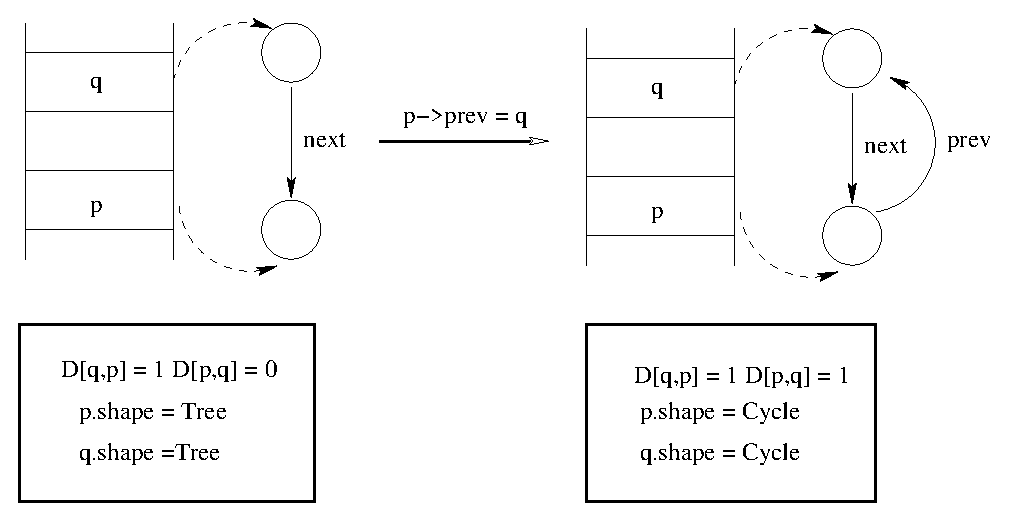
\includegraphics[scale=1]{Figure/figure_3}
}
\caption{Example Demonstrating Shape Estimation}
\label{fig:relwork_2}
\end{figure}

\subsection*{Analysis of Basic Statements}
They have considered eight basic statements that can access or
modify heap data structures as listed in Fig.~\ref{fig:relwork_3}(a). Variables \p\ and \q and the field $f$ are
of pointer type, variable $k$ is of integer type, and $op$ denotes the $+$ and $-$ operations. The 
overall structure of the analysis is shown in Fig.~\ref{fig:relwork_3}(b). Given the direction and the interference 
matrices $D$ and $I$ at a program point x, before the given statement, they compute the matrices $D_n$ and $I_n$
at a program point y. Additionally, we have the attribute matrix A, where for a pointer $p$, $A[p]$ gives its shape attribute.
The attribute matrix after the statement is presented as $A_n$.

For each statement they compute the set of direction and interference relationships it kills and generates. Using these sets, the
new matrices $D_n$ and $I_n$ are computed as shown in Fig.~\ref{fig:relwork_3}(c). Note that the elements in the gen and kill sets are denoted as $D[p,q]$
for direction relationships, and $I[p,q]$ for interference relationships. Thus a gen set of the form $\{D[x,y], D[y,z]\}$, indicates that
the corresponding entries in the output direction matrix $D_n[x,y]$ and $D_n[y,z]$ should be set to one. We also compute the set of 
pointers $H_s$, whose shape  attribute can be modified by the given statement. Another attribute matrix $A_c$ is used to store the 
changed attribute of pointers belonging to the set $H_s$. The attribute matrix $A_n$ is then computed using the 
matrices $A$ and $A_c$ as shown in Fig.~\ref{fig:relwork_3}(c).  

Let $H$ be the set of pointers whose relationships/attributes are abstracted by the matrices $D$. $I$ and $A$. Further
assume that updating an interference matrix entry $I[\q,\p]$, implies identically updating the entry $I[\p,\q]$.   
\begin{figure}
\centering
\scalebox{0.90}{
\begin{tabular}{|c|c|c|}
\hline
\begin{tabular}{l}
Allocation \\
1. {\tt p = malloc();} \\
\\
Pointer Assignments \\
2. {\tt p = q;} \\
3. {\tt p = \&(q$\rightarrow$f);} \\
4. {\tt p = q op k;} \\
5. {\tt p = NULL;} \\
6. {\tt p = q$\rightarrow$f;} \\
\\
Structure Updates \\
7. {\tt p$\rightarrow$f = q;} \\
8. {\tt p$\rightarrow$f = NULL;}
\end{tabular}  &
\begin{tabular}{c}
\scalebox{0.80}{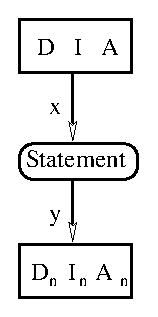
\includegraphics[scale=1]{diagrams/Appendix_4.eps}}
\end{tabular}
&
\begin{tabular}{l}
Build the new matrices\\
$\begin{array}{lll} 
\forall r,s \in H, & D_n[r,s] = D[r,s], & I_n[r,s] = I[r,s] \\
\forall s \in H, & A_n[s] = A[s]
\end{array}$ \\
\\
Delete Killed relationships \\
$\begin{array}{ll} 
\forall entries\ D[r,s] \in D\_kill\_set, & D_n[r,s] = 0\\  
\forall entries\ I[r,s] \in I\_kill\_set, & I_n[r,s] = 0\\  
\end{array}$ \\
\\
Add generated relationships \\
$\begin{array}{ll} 
\forall entries\ D[r,s] \in D\_gen\_set, & D_n[r,s] = 1\\  
\forall entries\ I[r,s] \in I\_gen\_set, & I_n[r,s] = 1\\  
\end{array}$ \\
\\
Update shape attributes of affected pointers \\
Compute $H_s$ and $A_s$ \\
$\begin{array}{ll} 
\forall s \in H_s, & A_n[s] = A[s]\\  
\end{array}$
\end{tabular}
\\
\scalebox{0.80}{(a) Basic statements} & \scalebox{0.80}{(b) Analysis Structure} & \scalebox{0.80}{(c) General Form of Analysis Rules} \\
\hline
\end{tabular}
}
\caption{The Overall Struture of the Analysis}
\label{fig:relwork_3} 
\end{figure}


The actual analysis rules can be divided into three groups: (1) allocations, (2) pointer assignments, and 
(3) structure updates. Figure~\ref{fig:relwork_4} shows the gen and kill sets corresponding to each statement. 
\begin{figure}[h]
\centering
\begin{tabular}{|l|c|}
\hline
1. {\tt p  = malloc();} &  
					$\begin{array}{lll}
						D\_kill\_set &=& \{D[p,s] \vert s \in H \wedge D[p,s]\}\ \cup\\
                                     &&   \{D[s,p] \vert s \in H \wedge D[s,p]\} \\
						I\_kill\_set &=& \{I[p,s] \vert s \in H \wedge I[p,s]\} \\
						D\_gen\_set &=& \{D[p,p]\} \quad I\_gen\_set = \{I[p,p]\} \\
						H_s &=& \{p\} \quad A_c[p] = Tree 	\\
					\end{array}$
								\\
\hline
\begin{tabular}{l}
2. {\tt p = q;} \\
3. {\tt p = \&(q$\rightarrow$f);} \\
4. {\tt p = q op k;} \\
\end{tabular}
 & 
				\begin{tabular}{l}
					Kill set same as that of {\tt p  = malloc();} \\
					$\begin{array}{lll}
						D\_gen\_set\_from &=& \{D[s,p] \vert s \in H \wedge s \not= p \wedge D[s,q]\} \\
						D\_gen\_set\_to &=& \{D[p,s] \vert s \in H \wedge s \not= p \wedge D[q,s]\} \\
						I\_gen\_set	&=& \{I[p,s] \vert s \in H \wedge s \not= p \wedge I[q,s]\}\ \cup \\
											&&  \{I[p,p] \vert I[q,q]\} \\
						D\_gen\_set	&=& D\_gen\_set\_from\ \cup D\_gen\_set\_to \\
						H_s &=& \{p\} \quad A_c[p] = A[q] 	\\
					\end{array}$
				\end{tabular}
								\\
\hline
5. {\tt p = NULL;} & 
				\begin{tabular}{l}
					Kill set same as that of {\tt p  = malloc();} \\
					$\begin{array}{lll}
						D\_gen\_set &=& \{\} \quad I\_gen\_set = \{\} \\
						H_s &=& \{p\} \quad A_c[p] = Tree 	\\
					\end{array}$
				\end{tabular}
								\\
\hline
6. {\tt p = q$\rightarrow$f;} & 
				\begin{tabular}{l}
					Kill set same as that of {\tt p  = malloc();} \\
					$\begin{array}{lll}
						D\_gen\_set\_from 	&=& \{D[s,p] \vert s \in H \wedge s \not= p \wedge I[s,q]\} \\
						D\_gen\_set\_to 	&=& \{D[p,s] \vert s \in H \wedge s \not= p \wedge s \not= q\ \wedge \\
                                            &&    D[q,s]\}\ \cup \{D[p,q] \vert A[q] = Cycle\}\ \cup \\
											&& \{D[p,p] \vert D[q,q]\} \\
						D\_gen\_set 		&=& D\_gen\_set\_from\ \cup D\_gen\_set\_to \\
						I\_gen\_set 		&=& \{I[p,s] \vert s \in H \wedge s \not= p \wedge I[q,s]\}\ \cup \\
											&&  \{I[p,p] \vert I[q,q]\} \\
						A_c[p] &=& A[q] 	\\
					\end{array}$
				\end{tabular}
								\\
\hline
7. {\tt p$\rightarrow$f = NULL;} & 
					$\begin{array}{lll}
						D\_kill\_set &=& \{\} \quad I\_kill\_set = \{\}\\
						D\_gen\_set 		&=& \{\} \quad I\_gen\_set  = \{\}\\
						A_c[p] &=& A[p]\ \forall p \in H  	\\
					\end{array}$
								\\
\hline
7. {\tt p$\rightarrow$f = q;} & 
				\begin{tabular}{l}
					Kill set same as that of {\tt p$\rightarrow$f = NULL;} \\
					$\begin{array}{lll}
						D\_gen\_set		&=& \{D[r,s] \vert r,s \in H \wedge D[r,p] \wedge D[q,s]\}  \\
						I\_gen\_set  	&=& \{I[r,s] \vert r,s \in H \wedge D[r,p] \wedge I[q,s]\} \\
					\end{array}$ \\ \\
					\underline{Pointer q already has a path to p, D[q,p] = 1} \\
					$\begin{array}{lll}
						H_s 			&=& \{s \vert s \in H \wedge (D[s,p] \vee D[s,q])\} \\
						D[q,p] &\Rightarrow& A_c[s] = Cycle\ \forall s \in H_s  	\\
					\end{array}$ \\ \\
					\underline{A[q] = Tree} \\
					$\begin{array}{lll}
						H_s 			&=& \{s \vert s \in H \wedge (D[s,p] \vee I[s,q])\} \\
						(\neg D[q,p] \wedge (A[q] = Tree)) &\Rightarrow& A_c[s] = A[s] \Join Dag\ \forall s \in H_s  	\\
					\end{array}$ \\ \\
					\underline{A[q] $\not=$ Tree} \\
					$\begin{array}{lll}
						H_s 			&=& \{s \vert s \in H \wedge D[s,p]\} \\
						(\neg D[q,p] \wedge (A[q] \not= Tree)) &\Rightarrow& A_c[s] = A[s] \Join A[q]\ \forall s \in H_s  	\\
					\end{array}$
				\end{tabular}
								\\
\hline							
\end{tabular}
\caption{Analysis Rules}
\label{fig:relwork_4}
\end{figure}


%%%%%%%%%%%%%%%%%%%%%%%%%%%%%%%%%%%%%%%%%%%%%%%%%%%%%%%%%%%%%%%%%%%%%%
\chapter[Analysis of Marron et. al.~\cite{marron06static}]{Analysis of Marron et. al.~\cite{marron06static}\footnote{The contents of this section are borrowed from ~\cite{marron06static}}}
%%%%%%%%%%%%%%%%%%%%%%%%%%%%%%%%%%%%%%%%%%%%%%%%%%%%%%%%%%%%%%%%%%%%%%
Most of the technical terms used in this chapter are borrowed from the aforementioned paper.
The proposed analysis followed the abstract heap graph model that uses nodes to
represent sets of concrete cells (heap allocated objects and arrays) and edges to represent sets of pointers. 
Each node in the abstract heap graph can be viewed as a region in memory on which certain
layout predicates can be defined (Tree Layout, List Layout, Singleton Layout, Multi-Path or Cycle Layouts)
which signifies what types traversal patterns a program can use to navigate through the data
structures in the region. To track the concrete Structure Layout, they introduce a simple domain of 
layout types = \{Singleton, List, Tree, Multi-Path, Cycle\}. The abstract layouts can be given a simple
total order: Singleton < List < Tree < Multi-Path < Cycle. This order can be interpreted as: if
a node n has abstract layout $\zeta$ then the concrete region, $\mathcal{R} = \gamma(n)$, where $\gamma$ is the concreatization
operator, may have any of the layout properties less than or equal to $\zeta$. For example, if we have a node
with layout type List the concrete region may have the List or Singleton layout properties. If the
node has Cycle as the layout then the concrete domain may have any of the layout properties. The
abstract layout for a node n represents the most general concrete layout that may be encountered
by a program traversing the region that is represented by the node n.

In their analysis, sometimes refinement is necessary (after summarization the abstract heap graph) whose 
purpose is to transform summary representations into forms that make certain relationships explicit, so that the information
 in these relationships can be utilized more easily. During refinement they turn summary nodes 
into a number of nodes of size one so that strong updates can be performed and exact relations 
between variables can be maintained. 

In order to eliminate the state explosion that is possible with refinement, they adopt the approach
of only doing refinement in those cases in which we can be sure that there is a unique way in which
new nodes can be materialized. This limits the level of details that can be achieved, but it 
is easy to demonstrate scenarios where refinement into multiple possibilities is needed to get results with the
desired accuracy. 


\bibliographystyle{alpha}
\bibliography{Report}
\end{document}


